%% thesis.tex 2022/2/14
%
% Based on sample files of unknown authorship.
%
% The San Francisco State University LaTeX thesis template is
% derived from the UC Berkeley LaTeX thesis template. 
%
% The current maintainer of this work at San Francisco State University is Robert Browder.
%
% A healthy alternative to working directly in LaTeX is to use the thesisdown or bookdown package with R Studio.
% Thesis down provides the opportunity to embed executable code within the narrative flow of your document.
% Thesis down provides both PDF and HTML output.  
%
% This is the main file for this template
%
% This file is where authors may customize title, author, degree semester, degree year, degree, 
% chair, other members, and major.
%
% This file issues the commands to include each part of the document, 
% Pre-formatted parts available - abstract, preface, acknowledgments, introduction, chap1, chap2, 
% and references
% Any part can be omitted by commenting out its "include" command
% Authors may also rearrange the order of contents and add additional chapters using the mark-up examples provided


\documentclass{sfsuthesis}
% see https://www.overleaf.com/learn/latex/Articles/Getting_started_with_BibLaTeX for more info
\usepackage[backend=biber,style=numeric]{biblatex}
\addbibresource{references.bib} % the file containing your citations

% Use the graphix package with dvipdfmx when exporting to HTML to preserve figure dimensions for JPG and PNG file types. 
% For this to work you must first create an .xbb file for each file using the following command from the CLI
% ebb -x Picture2.jpg
% \usepackage[dvipdfmx]{graphicx}

% Use the graphix package without dvipdfmx when exporting to PDF
\usepackage{graphicx}
\usepackage{amsmath}
\usepackage{rotating} % provides sidewaystable and sidewaysfigure
\usepackage{lipsum}
\usepackage{subcaption}
\usepackage{booktabs, multirow}
\usepackage{caption}
\usepackage{longtable}
% \usepackage[tagged]{accessibility}

% To compile this file from the command line, run "latex thesis", then "biber thesis"
% (or "bibtex thesis", if the output from latex asks for that instead),
% and then "latex thesis" (without the quotes in each case).
%
% Alternatively, use Overleaf, MacTeX, or MikTeX to compile to PDF.
%
% To compile this file to HTML from the command line, run 
%  make4ht -f html5+mjcli thesis.tex "mathjax"
% this step requires Nodes.js, MathJax, and mjcli.js to be installed and working on your machine


% comment out the following two lines for single spacing
\def\dsp{\def\baselinestretch{2.0}\large\normalsize}
\dsp

% comment out the following line to control indentation of the first paragraph of a section
\usepackage{indentfirst}
\usepackage{appendix}

%% ewb 3/2024 additions
\usepackage{physics}    
\usepackage{comment}    
\usepackage{color}      
\usepackage{listings}

\usepackage{csquotes} % Recommended with biblatex
\PassOptionsToPackage{hyphens}{url}
\usepackage{hyperref}

\DeclareFieldFormat{url}{\url{#1}}
\renewcommand*{\biburlsetup}{\Urlmuskip=0mu plus 1mu\relax}
\setcounter{biburlnumpenalty}{9000}
\setcounter{biburlucpenalty}{9000}
\setcounter{biburllcpenalty}{9000}

% for code formatting/coloring
\definecolor{codegreen}{rgb}{0,0.6,0}
\definecolor{codegray}{rgb}{0.5,0.5,0.5}
\definecolor{codepurple}{rgb}{0.58,0,0.82}
\definecolor{backcolour}{rgb}{0.95,0.95,0.92}
\definecolor{codecyan}{rgb}{0.0,0.2,1.0}

% see: https://en.wikibooks.org/wiki/LaTeX/Source_Code_Listings
% set font, size, color style for code listings
\lstdefinestyle{mystyle}{
%    backgroundcolor=\color{backcolour},
    commentstyle=\textcolor{codegreen},
%    keywordstyle=\color{magenta},
    keywordstyle=\color{codecyan},
    numberstyle=\tiny\color{codegray},
    stringstyle=\color{codepurple},
    basicstyle=\ttfamily\footnotesize,
    breakatwhitespace=false,
    breaklines=true,
    captionpos=b,
    keepspaces=true,
    numbers=left,
    numbersep=2pt,
    firstnumber=auto,
    numberblanklines=false,
    showspaces=false,
    showstringspaces=false,
    showtabs=false,
    tabsize=2
}
% and then set mystyle to be the default when doing code listings
\lstset{style=mystyle}


%% end ewb 3/2024 addition

\addtolength{\abovecaptionskip}{\baselineskip}

\newtheorem{theorem}{Sample Text}

\bibliography{references}

\hyphenation{mar-gin-al-ia}
\hyphenation{bra-va-do}

%path to the folder which contains figures
\graphicspath{ {./figures/} }

\begin{document}
% \emergencystretch 5em
% Declarations for Front Matter

\title{Automating Course Articulation\\\vspace*{2mm}\large A Deep Metric Learning Framework Using Public Data}
\makeatletter
\newcommand{\@approvaltitle}{Automating Course Articulation: A Deep Metric Learning Framework Using Public Data}
\makeatother
% Automating Course Transferability: A Deep Embedding and Traditional Classifier Approach
\author{Mark S. Kim}
\degreesemester{May}
% Select one of the semesters: December, May, or August.
\degreeyear{2025}
% Enter the year in which you are submitting your thesis.
\degree{Master of Science}
%example: Masters of Science
\chair{Hui Yang}
\chairdegree{Ph.D}
\chairrank{Professor}
\cochair{Arno Puder}
\cochairdegree{Ph.D}
\cochairrank{Professor}
\memberthree{Anagha Kulkarni}
\memberthreedegree{Ph.D}
\memberthreerank{Professor}
% \memberfour{Name of Member Four}
% \memberfourdegree{Ph.D}
% \memberfourrank{Associate Professor}
% \othermembers{Professor Roger Spam \\
%   Associate Professor Michael Chex}
% For a co-chair who is subordinate to the \chair listed above
% \cochair{Professor Benedict Francis Pope}
% For two co-chairs of equal standing (do not use \chair with this one)
% \cochairs{Professor Richard Francis Sony}{Professor Benedict Francis Pope}
\numberofmembers{3}

\field{Data Science and Artificial Intelligence}
% Example: Computer Science: Software Engineering
% Designated Emphasis -- this is optional, and rare
% \emphasis{Colloidal Telemetry}
% This is optional, and rare
% \jointinstitution{University of Western Maryland}
% This is optional (default is Berkeley)
% \campus{Berkeley}


\maketitle
% Delete (or comment out) the \approvalpage line for the final version.
\copyrightpage
\approvalpage


% (This file is included by thesis.tex; you do not latex it by itself.)
\begin{abstract}

% The text of the abstract goes here.  If you need to use a \section
% command you will need to use \section*, \subsection*, etc. so that
% you don't get any numbering.  You probably won't be using any of
% these commands in the abstract anyway.

\lipsum[1]

\end{abstract}


\begin{frontmatter}

    % \begin{preface}

\end{preface}

    % You can delete the \clearpage lines if you don't want these to start on
    % separate pages.


    \begin{acknowledgments}
I would like to express my deepest appreciation to my advisors, Professors Hui Yang, Arno Puder, and Anagha Kulkarni. Their patience, support, and confidence in me were invaluable throughout my graduate journey at SFSU. I also owe a special debt of gratitude to Professor Tao He, whose crucial suggestion to incorporate a global similarity metric with the embedding vectors significantly improved the model's classification performance.

This research was made possible through the contributions of many individuals. I'd like to thank the Program Pathways Mapper (PPM) team, which includes representatives from the Kern Community College District, the Foundation for California Community Colleges, and the California Community Colleges Chancellor's Office, for their partnership in providing the foundational data for this work.  I'd like to recognize Natalie Yam, Parth Panchal, and Joanne Park for their assistance with data collection, compilation, and preliminary analysis.

This work was supported in part through the Platform for Open Learning, Academic Research, \& Innovative Scientific computing (POLARIS) High-Performance Computing (HPC) cluster at San Francisco State University. We acknowledge these resources, services, and the support provided by the Academic Technology Systems Team.

On a personal note, I am immensely thankful for my dear friends who have been there for me through thick and thin, cheering me on whenever I felt I could not continue. To my good friend, Phil, I offer my deepest appreciation for his incredible generosity and support, which made navigating the financial challenges of graduate school possible. To Julie and Bita, I am profoundly thankful for their invaluable guidance and perspective, which were instrumental to my personal growth and well-being throughout this journey.  To my brother Nick, I am eternally grateful for his quiet strength and unwavering support during times when distance and understanding meant everything.

To all who stood by me with patience, kindness, and belief---I carry your support with deep gratitude.
\end{acknowledgments}

    \tableofcontents
    \clearpage
    \listoftables
    \clearpage
    \listoffigures
    \clearpage

\end{frontmatter}

% % (This file is included by thesis.tex; you do not latex it by itself.)

\begin{introduction}

    % If you need to use a \section
    % command you will need to use \section*, \subsection*, etc. so that
    % you don't get any numbering.  You probably won't be using any of
    % these commands in the abstract anyway.
    % \section{California's Transfer Maze: An Archetype for a National Problem}

    California's public higher education system is a titan of American academia, a complex, three-tiered structure comprising the University of California (UC), California State University (CSU), and the California Community Colleges (CCC)~\cite{ppic}. Collectively, these 149 colleges and universities serve nearly 2.9 million students, forming the largest public higher education system in the United States~\cite{ppic,uc,calstate,cccco}. A foundational principle of this system is the promise of student mobility, particularly the pathway from a two-year community college to a four-year university. However, the mechanism designed to facilitate this movement, the process of determining course equivalency, or articulation, is a formidable, largely manual process that creates significant barriers for students.

    At the heart of this process is the Articulation System Stimulating Interinstitutional Student Transfer (ASSIST), the state's official public repository for articulation agreements~\cite{assistinfo}. While ASSIST provides a centralized platform for students and advisors to view established equivalencies, it is fundamentally a display for agreements that are negotiated and updated manually by articulation officers at each individual campus~\cite{assistfaq}. Given the sheer number of institutions, the process of defining and maintaining these agreements is a task of bleak combinatorics, rendering it inefficient, slow, and inherently intractable~\cite{pardos2019}. This manual paradigm places a considerable burden on academic advisors and administrative staff, who must meticulously review course descriptions and syllabi to compare content, rigor, and learning outcomes~\cite{pardos2019}. The result is a system that struggles to keep pace with the needs of a vast and mobile student body, making California a critical case study for a problem that extends far beyond its borders.

    The challenges exemplified by California's system are a microcosm of a systemic crisis in American higher education. The act of transferring between institutions has become a normative component of the modern student's academic journey. Data from the National Student Clearinghouse Research Center reveals that in the fall of 2023, transfer enrollment constituted 13.2\% of all continuing and returning undergraduates~\cite{nscnews2023}. This trend is not static; it represents a post-pandemic resurgence in student mobility, with transfer enrollment growing by 5.3\% from Fall 2022 to Fall 2023 and an additional 4.4\% in Fall 2024~\cite{nscnews2023,nscnews20250305}. This mobile population is increasingly diverse, comprising not only students following traditional two-year to four-year pathways but also a substantial number of returning learners who have previously paused their education. Over half of these returning students opt to re-enroll at a new institution, underscoring the critical role of the transfer system in providing flexible pathways to degree completion~\cite{nscdd20250507}.

    The consequences of this systemic inefficiency are borne almost entirely by the students, manifesting in significant academic and financial setbacks. The most direct and damaging outcome is the loss of earned academic credit. A comprehensive 2017 report by the U.S. Government Accountability Office (GAO) estimated that students who transferred between 2004 and 2009 lost an average of 43\% of their credits in the process~\cite{gao2017}. This finding is echoed across numerous studies, with reports indicating that more than half of all transfer students lose at least some credits, and approximately one-fifth are forced to repeat courses for which they have already received a passing grade at a previous institution~\cite{publicagenda2025}.

    This loss of credit creates a cascade of negative consequences. It invariably leads to an increased time-to-degree, delaying graduation and entry into the workforce. Each repeated course also carries a financial cost, increasing the total tuition burden and potentially exhausting a student's eligibility for federal financial aid programs like Pell Grants and Direct Loans~\cite{gao2017}. A process that is often undertaken to save money (for example, by starting at a less expensive community college) can paradoxically result in a greater overall financial commitment, trapping students in a cycle of additional coursework and debt~\cite{collegeopportunity2017}.

    The friction and frustration inherent in the transfer process also have a measurable impact on student persistence and graduation. Studies have shown that transfer students, as a group, tend to have lower retention and graduation rates than their peers who begin and end their studies at the same institution~\cite{porter1999}. This issue transcends mere administrative inefficiency and becomes a critical matter of educational equity. Low-income students and students from historically underrepresented racial and ethnic groups are more likely to begin their postsecondary journey at community colleges and rely on transfer pathways to attain a bachelor's degree~\cite{ace2025}. The recent growth in transfer enrollment has been driven disproportionately by Black and Hispanic students~\cite{nscnews2023}. Therefore, the barriers imposed by an inefficient articulation system such as credit loss, increased cost, and delayed graduation, disproportionately harm the very student populations that institutions are striving to support.

    A clear and troubling feedback loop emerges from this analysis. The fundamentally manual and inefficient nature of course articulation is a direct cause of credit loss. This credit loss imposes a tangible academic and financial burden on students which falls most heavily on underrepresented and low-income students, who are a large and growing segment of the transfer population. This disproportionate impact, in turn, undermines institutional goals of improving student retention and closing persistent equity gaps in degree attainment. Thus, the seemingly low-level administrative task of determining course equivalency is revealed to be a significant driver of systemic inequity in higher education. Addressing this challenge through robust automation is not merely an operational optimization; it is a necessary intervention to foster a more equitable, efficient, and supportive educational ecosystem for all students.

    \section{The Call for Automation}\label{sec:automation}
    The manifest inefficiencies and inequities of manual course articulation, exemplified by the challenges within California's vast system, have prompted a range of research efforts aimed at automating the process~\cite{ma_course_recommendation_2017, PardosCourse2Vec2019, pardos-articulation-2019, JiangPardosMulti2VecEDM2020,XuPardosSubwordEmbeddings2024}. These technological interventions have evolved in sophistication, mirroring the broader advancements in natural language processing (NLP) and machine learning. A critical review of this literature reveals a clear trajectory from simple statistical methods to complex deep learning models, with each stage introducing new capabilities while also exposing new limitations. This evolution illuminates the path toward a more robust and scalable solution.

    \subsection{Foundational Approaches: Keyword and Statistical Methods}
    The earliest attempts at automating course comparison relied on foundational text analysis techniques that, while computationally simple, lack semantic depth. The most basic systems are essentially search engines or databases that depend on exact keyword matching or pre-populated tables of known equivalencies~\cite{shamrock}. These systems are inherently brittle; they cannot recognize semantic variations (e.g., equating ``Introduction to Programming'' with ``Fundamentals of Computer Science I'') and require continuous manual updates to remain relevant~\cite{shiferaw2024}.

    A more advanced statistical method, Term Frequency-Inverse Document Frequency (TF-IDF), improves upon keyword matching by vectorizing documents and weighting terms based on their importance. A term's frequency within a single document (TF) is balanced against its rarity across a collection of documents, or corpus (IDF)~\cite{AIZAWA200345}. This allows the model to assign higher importance to distinctive terms (e.g., ``calculus'') and lower importance to common words (e.g., ``the,'' ``a,'' ``is'')~\cite{AIZAWA200345}. TF-IDF has been a workhorse for information retrieval and has been applied to course similarity tasks~\cite{AIZAWA200345}. However, the fundamental limitation of TF-IDF and other bag-of-words models is their complete lack of semantic understanding. They treat words as discrete, unrelated tokens and cannot grasp that ``calculus'' and ``differentiation'' are related concepts, nor can they distinguish between different meanings of the same word.

    \subsection{Static Semantic Representations}
    The development of word embeddings represented the first major leap toward a true semantic understanding of course content. Models like Word2Vec and GloVe, trained on vast text corpora, learn to represent words as dense vectors in a high-dimensional space, where words with similar meanings are positioned closer to one another. For example, the vectors for ``car'' and ``automobile'' would be near each other, while being distant from the vector for ``planet.'' This innovation enabled a more nuanced comparison of texts than was possible with TF-IDF. In the context of educational data mining, these techniques have been applied to content-based course recommendation systems, typically by creating a single vector representation for a course description by averaging the vectors of all its constituent words~\cite{pardos10.1145/3330430.3333622}.

    Despite this advancement, these models produce static embeddings. Each word is assigned a single, fixed vector regardless of its context. This is a significant drawback, as it fails to account for polysemy: words with multiple meanings. For instance, the word ``bank'' would have the same vector in the phrases ``river bank'' and ``bank account,'' despite their disparate meanings. Furthermore, the common practice of averaging all word vectors to create a document-level representation is a crude heuristic that can dilute or lose critical semantic information, especially in complex or lengthy descriptions.

    \subsection{Contextual Semantic Representations}
    The introduction of the transformer architecture, and specifically models like Bidirectional Encoder Representations from Transformers (BERT), revolutionized NLP by enabling the generation of contextual embeddings. In these models, the vector representation of a word is dynamically influenced by the words surrounding it in a sentence~\cite{devlin2019bertpretrainingdeepbidirectional}. This allows the model to disambiguate word meanings and capture a much richer, more accurate semantic representation of the text. Architectures such as Sentence-BERT (SBERT) were subsequently developed to fine-tune these models specifically for the task of producing semantically meaningful embeddings for entire sentences or short paragraphs, which can then be efficiently compared using metrics like cosine similarity~\cite{reimers2019sentencebertsentenceembeddingsusing}.

    The most recent evolution in this domain involves the direct application of large-scale generative models, or Large Language Models (LLMs) like GPT-4 and Gemini, for classification tasks. Through sophisticated prompt engineering and in-context learning, these models can be instructed to perform pairwise comparisons of course descriptions and render a judgment on their equivalency. The preliminary work for this thesis explored this very approach, using Google's Gemini Pro to classify course pairs. While these experiments yielded promising accuracy, they also uncovered significant practical and theoretical limitations. The direct use of LLMs for this task is computationally expensive and inefficient, as it requires repeatedly sending full text descriptions to a model API for every comparison. Performance is acutely sensitive to the exact phrasing of the prompt, necessitating a costly and time-consuming iterative tuning process. Most critically, the decision-making process of an LLM is a ``black box,'' providing a categorical output (e.g. ``equivalent'') without a quantifiable similarity score or confidence level. This opacity makes it difficult to rank potential matches, set decision thresholds, or provide transparent justifications for the model's conclusions. This approach is also ill-suited for handling more complex articulation scenarios, such as one-to-many or many-to-many course mappings.

    \subsection{Enrollment-Based Approaches}
    It is essential to situate this research within the context of parallel efforts that leverage different data sources. A notable body of work has demonstrated that course similarity and prerequisite relationships can be predicted with high accuracy by analyzing student enrollment data. Models such as \emph{course2vec} learn course embeddings not from their textual descriptions, but from the patterns of which courses students tend to take together~\cite{pardos2018connectionistrecommendationwildutility}. The underlying principle is that courses frequently taken in the same semester or in sequence likely share a functional or topical relationship~\cite{pardos2018connectionistrecommendationwildutility}.

    While this behavioral approach is powerful, its reliance on large-scale, proprietary institutional datasets of student records presents two major obstacles. First, it raises significant data privacy and security concerns, as it involves the analysis of sensitive student information~\cite{slade10.1177/0002764213479366}. Second, it limits the scalability and generalizability of the solution. The model is only applicable at institutions that can provide access to such data, and it cannot be used to compare courses between two institutions that have no history of student transfer between them. This approach is therefore not a universal solution for the broader course articulation problem.

    The evolution of these varied approaches reveals a fundamental trade-off: as models gain greater semantic power, they tend to become more computationally intensive, less interpretable, and more demanding of specialized or private data. The limitations of direct LLM classification (cost, opacity) and enrollment-based methods (data privacy, limited access) point toward the need for a new paradigm. An ideal solution should harness the semantic power of large pre-trained models without inheriting their operational burdens. This suggests that the next logical step is not simply a larger, more complex end-to-end model, but rather a more intelligent, hybrid framework. Such a framework would decouple the task of deep semantic representation from the task of final classification, allowing each component to be optimized for what it does best. This conceptual shift forms the central motivation for the methodology proposed in this thesis.  Table~\ref{tbl:taxonomy} summarizes the primary methods for determining course transferability.

    \begin{table}[!htb]
        \centering
        \setlength{\tabcolsep}{10pt} % Default value: 6pt
        \renewcommand{\arraystretch}{1.5}  % Provide more space between table rows, if you prefer
        \caption{Comparative Taxonomy of Course Equivalency Determination Methods}\label{tbl:taxonomy}
        \resizebox{\columnwidth}{!}{
            \begin{tabular}{>{\raggedright\arraybackslash}p{2.25cm}>{\raggedright\arraybackslash}p{3cm}>{\raggedright\arraybackslash}p{1.75cm}>{\raggedright\arraybackslash}p{1.9cm}>{\raggedright\arraybackslash}p{3.75cm}>{\raggedright\arraybackslash}p{3.75cm}}
                \toprule
                Approach                                       & Key Characteristics                                                   & Data Source(s)              & Semantic Capability & Strengths                                                                                  & Limitations                                                                                                                   \\
                \midrule
                Manual Review                                  & Human experts (advisors, faculty) compare syllabi descriptions.       & Course Catalogs, Syllabi    & High (Human-level)  & Nuanced, context-aware, trusted by faculty.                                                & Extremely slow, not scalable, subjective, prone to inconsistency.                                                             \\
                Keyword/ TF-IDF                                & Bag-of-words representation, statistical term weighting.              & Course Catalogs             & None to Low         & Simple, computationally cheap, easy to implement.                                          & Fails to capture synonyms, context, or true semantic meaning                                                                  \\
                Static\hspace{3em}Embeddings (Word2Vec/ GloVe) & Pre-trained word vectors, often averaged for document representation. & Course Catalogs             & Medium              & Captures word-level semantics, better than TF-IDF.                                         & Context-insensitive, averaging vectors loses information.                                                                     \\
                Enrollment-Based (e.g., course2vec)            & Embeddings learned from student co-enrollment patterns.               & Proprietary Student Records & High (Behavioral)   & Captures functional relationships between courses, highly predictive.                      & Requires access to sensitive private data, not generalizable, privacy concerns.                                               \\
                Direct LLM Classification                      & End-to-end classification using prompt engineering.                   & Course Catalogs             & Very High           & High accuracy potential, understands complex language.                                     & Computationally expensive, ``black box'' opacity, prompt sensitive, no quantifiable similarity score, risk of hallucinations. \\
                Proposed Method (Embeddings + ML)              & Deep contextual embeddings as features for traditional classifiers.   & Course Catalogs             & Very High           & State-of-the-art accuracy, computationally efficient, quantifiable, uses public data only. & Relies on the quality of the pre-trained embedding model.                                                                     \\
                \bottomrule
                % \multicolumn{4}{p{6cm}}{\scriptsize $^{*}$ Huggingface Overall Leaderboard Rank}      \\
                % \multicolumn{4}{p{6cm}}{\scriptsize $^{\dagger}$ in Millions}
            \end{tabular}
        }
    \end{table}

\section{Embedding-Based Classification}\label{sec:embclass}
In response to the limitations of existing methods, this thesis proposes and validates a novel framework for automating course equivalency determination. This approach is designed to achieve state-of-the-art accuracy while remaining computationally efficient, transparent, and reliant only on publicly available data. It achieves this by strategically decoupling the process of semantic understanding from the final classification task, leveraging the distinct strengths of deep embedding models and traditional machine learning classifiers.

\subsection{Feature Engineering Engine}
The foundational principle of the proposed framework is to utilize state-of-the-art deep embedding models not as end-to-end classifiers, but as highly sophisticated feature extraction engines. In this paradigm, a publicly available course description, in its raw text form, is processed by a pre-trained contextual embedding model. The model's task is to convert the unstructured text into a high-dimensional numerical vector that encapsulates the rich semantic content of the course.

This computation is performed once for each course in the catalog, transforming the entire corpus of unstructured text into a structured database of semantic vectors. This pre-processing step creates a reusable and efficient representation of each course, directly addressing the primary drawbacks of the direct LLM classification approach. By storing these embeddings, the framework eliminates the need to repeatedly process the same raw text through a costly API, drastically reducing computational overhead and latency for subsequent comparisons. This makes the system inherently more scalable and suitable for real-world applications that may involve hundreds of thousands of courses.

\subsection{Distance Metric for Classification}
A central innovation of this research lies in the method used to compare two course embeddings. Preliminary analysis revealed that relying on a single, holistic similarity metric like cosine similarity was insufficient for establishing a clear and reliable decision boundary between equivalent and non-equivalent course pairs. To overcome this, a composite distance vector was developed to serve as a richer feature set for the classification model.

This feature vector, denoted as \(\Delta_c\), is constructed by concatenating the element-wise difference of the two course embedding vectors (\(\mathbf{A}\) and \(\mathbf{B}\)) with their cosine similarity. The formal definition is as follows:
\[ \Delta_c = \left(a_1 - b_1, \dots, a_k - b_k, \frac{\mathbf{A}\cdot\mathbf{B}}{\parallel \mathbf{A} \parallel \parallel \mathbf{B} \parallel } \right) \]
where \(\mathbf{A} = (a_1, \dots, a_k) \) and \(\mathbf{B} = (b_1, \dots, b_k) \) are the \(k\)-dimensional embedding vectors for the two courses.  This design is powerful because it provides the subsequent classifier with two distinct types of information simultaneously. The element-wise difference captures granular, dimension-specific (local) disparities between the two semantic representations, while the cosine similarity provides a single, normalized measure of their overall (global) alignment in the vector space. This composite vector creates a much more informative and discriminative feature set than a single similarity score alone.

\subsection{Classical Machine Learning}
By transforming the comparison of two courses into the generation of a fixed-length feature vector (\(\Delta_c\)), the complex problem of semantic evaluation is effectively reduced to a standard, supervised classification task. This allows for the application of a suite of well-understood and highly optimized traditional machine learning algorithms. In this research, models including Logistic Regression, Support Vector Machines (SVM), k-Nearest Neighbors (k-NN), and Random Forests (RF) were trained on these generated distance vectors to predict a binary label: equivalent or not equivalent.

This hybrid approach demonstrates remarkable efficacy. Experimental results show that the non-linear models, in particular, achieve exceptional performance. Across various embedding models and dimensionality reduction techniques, models such as k-NN, SVM, and RF consistently produced \(F_1\)-scores ranging from 0.971 to an exceptionally high 0.996. This level of accuracy represents a significant improvement over previously reported methods and may achieve the level of reliability required for a production system.

Furthermore, this framework proves to be highly efficient. A key finding is that smaller, more computationally modest fine-tuned embedding models (e.g.\ the 33-million-parameter BGE model) can achieve performance that is comparable to, and in some cases better than, general pre-trained models that are orders of magnitude larger and more complex (e.g.\ the 7.8-billion-parameter NV-EmbedV2 a model) when used within this framework.  This has profound practical implications, suggesting that state-of-the-art results can be achieved without requiring massive computational resources or reliance on proprietary, closed-source models. Finally, this approach offers a degree of interpretability that is absent in end-to-end LLM solutions. Models like Random Forest can provide feature importance metrics, offering insights into which dimensions of the semantic space are most critical for determining equivalency, thereby opening the ``black box'' of the decision-making process.

\section{Contributions}
This research makes several key contributions to the fields of educational data mining and natural language processing, offering a practical and powerful solution to the long-standing challenge of course articulation.

\subsection{Primary Contributions}
\begin{enumerate}
\item \textbf{A High-Accuracy, Automated Framework}: This thesis develops and validates a novel framework for determining course equivalency that achieves state-of-the-art accuracy, with \(F_1\)-scores exceeding 0.99 on a challenging real-world dataset. Crucially, it accomplishes this using only publicly available course catalog text, making it broadly applicable.
\item \textbf{An Innovative Feature Engineering Technique}: It introduces a composite distance vector, \(\Delta_c\), that uniquely combines element-wise embedding differences with cosine similarity. This technique provides a richer input signal for classification and is shown to demonstrably improve the performance of downstream machine learning models, particularly linear classifiers.
\item \textbf{A Computationally Efficient and Scalable Approach}: The research demonstrates that by decoupling semantic representation from classification, it is possible to harness the power of deep contextual embeddings without the high computational costs, API dependencies, and opaque nature of direct LLM-based classification. This makes the proposed solution more efficient, scalable, and practical for institutional deployment.
\item \textbf{A Privacy-Preserving Methodology}: By relying exclusively on public course descriptions, the proposed method circumvents the significant privacy, security, and data access challenges associated with techniques that require sensitive student enrollment records. This makes the framework more ethically sound and generalizable across any pair of institutions, regardless of their data-sharing agreements.
\end{enumerate}

\subsection{Thesis Roadmap}
The remainder of this thesis is structured to provide a comprehensive account of this research.
\begin{enumerate}
\item \textbf{Chapter 1: Background and Literature Review} will provide a detailed expansion of the topics covered in Sections~\ref{sec:automation} and~\ref{sec:embclass}, offering an in-depth survey of the student transfer landscape and the evolution of technological interventions.
\item \textbf{Chapter 2: Methodology} will offer a deep dive into the data collection and preparation processes, the specific embedding models evaluated, the construction of the feature vectors, and the theoretical underpinnings of the machine learning classifiers employed.
\item \textbf{Chapter 3: Experimental Setup and Results} will detail the experimental design, the datasets used for training and validation, and a comprehensive analysis of the classification performance, including ablation studies and model comparisons.
\item \textbf{Chapter 4: Discussion and Future Work} will interpret the results in a broader context, discuss the limitations of the current study, and outline promising avenues for future research, including the development of a full-scale course recommendation system and the exploration of fine-tuning techniques.
\item \textbf{Chapter 5: Conclusion} will summarize the key findings of the thesis and reiterate the significance of its contributions to both academic research and the practical administration of higher education.
\end{enumerate}

\end{introduction}


\pagestyle{headings}

% (Optional) \part{First Part}

\chapter{
    Introduction
    }

California's public higher education system is a titan of American academia, a complex, three-tiered structure comprising the University of California (UC), California State University (CSU), and the California Community Colleges (CCC)~\cite{ppic}. Collectively, these 149 colleges and universities serve nearly 2.9 million students, forming the largest public higher education system in the United States~\cite{ppic,uc,calstate,cccco}. A foundational principle of this system is the promise of student mobility, particularly the pathway from a two-year community college to a four-year university. However, the mechanism designed to facilitate this movement, the process of determining course equivalency, or articulation, is a formidable, largely manual process that creates significant barriers for students.

At the heart of this process is the Articulation System Stimulating Interinstitutional Student Transfer (ASSIST), the state's official public repository for articulation agreements~\cite{assistinfo}. While ASSIST provides a centralized platform for students and advisors to view established equivalencies, it is fundamentally a display for agreements that are negotiated and updated manually by articulation officers at each individual campus~\cite{assistfaq}. Given the sheer number of institutions, the process of defining and maintaining these agreements is a task of bleak combinatorics, rendering it inefficient, slow, and inherently intractable~\cite{pardos2019}. This manual paradigm places a considerable burden on academic advisors and administrative staff, who must meticulously review course descriptions and syllabi to compare content, rigor, and learning outcomes~\cite{pardos2019}. The result is a system that struggles to keep pace with the needs of a vast and mobile student body, making California a critical case study for a problem that extends far beyond its borders.

The challenges exemplified by California's system are a microcosm of a systemic crisis in American higher education. The act of transferring between institutions has become a normative component of the modern student's academic journey. Data from the National Student Clearinghouse Research Center reveals that in the fall of 2023, transfer enrollment constituted 13.2\% of all continuing and returning undergraduates~\cite{nscnews2023}. This trend is not static; it represents a post-pandemic resurgence in student mobility, with transfer enrollment growing by 5.3\% from Fall 2022 to Fall 2023 and an additional 4.4\% in Fall 2024~\cite{nscnews2023,nscnews20250305}. This mobile population is increasingly diverse, comprising not only students following traditional two-year to four-year pathways but also a substantial number of returning learners who have previously paused their education. Over half of these returning students opt to re-enroll at a new institution, underscoring the critical role of the transfer system in providing flexible pathways to degree completion~\cite{nscdd20250507}.

The consequences of this systemic inefficiency are borne almost entirely by the students, manifesting in significant academic and financial setbacks. The most direct and damaging outcome is the loss of earned academic credit. A comprehensive 2017 report by the U.S. Government Accountability Office (GAO) estimated that students who transferred between 2004 and 2009 lost an average of 43\% of their credits in the process~\cite{gao2017}. This finding is echoed across numerous studies, with reports indicating that more than half of all transfer students lose at least some credits, and approximately one-fifth are forced to repeat courses for which they have already received a passing grade at a previous institution~\cite{publicagenda2025}.

This loss of credit creates a cascade of negative consequences. It invariably leads to an increased time-to-degree, delaying graduation and entry into the workforce. Each repeated course also carries a financial cost, increasing the total tuition burden and potentially exhausting a student's eligibility for federal financial aid programs like Pell Grants and Direct Loans~\cite{gao2017}. A process that is often undertaken to save money (for example, by starting at a less expensive community college) can paradoxically result in a greater overall financial commitment, trapping students in a cycle of additional coursework and debt~\cite{collegeopportunity2017}.

The friction and frustration inherent in the transfer process also have a measurable impact on student persistence and graduation. Studies have shown that transfer students, as a group, tend to have lower retention and graduation rates than their peers who begin and end their studies at the same institution~\cite{porter1999}. This issue transcends mere administrative inefficiency and becomes a critical matter of educational equity. Low-income students and students from historically underrepresented racial and ethnic groups are more likely to begin their postsecondary journey at community colleges and rely on transfer pathways to attain a bachelor's degree~\cite{ace2025}. The recent growth in transfer enrollment has been driven disproportionately by Black and Hispanic students~\cite{nscnews2023}. Therefore, the barriers imposed by an inefficient articulation system such as credit loss, increased cost, and delayed graduation, disproportionately harm the very student populations that institutions are striving to support.

A clear and troubling feedback loop emerges from this analysis. The fundamentally manual and inefficient nature of course articulation is a direct cause of credit loss. This credit loss imposes a tangible academic and financial burden on students which falls most heavily on underrepresented and low-income students, who are a large and growing segment of the transfer population. This disproportionate impact, in turn, undermines institutional goals of improving student retention and closing persistent equity gaps in degree attainment. Thus, the seemingly low-level administrative task of determining course equivalency is revealed to be a significant driver of systemic inequity in higher education. Addressing this challenge through robust automation is not merely an operational optimization; it is a necessary intervention to foster a more equitable, efficient, and supportive educational ecosystem for all students.

\section{Contributions}
This research makes several key contributions to the fields of educational data mining and natural language processing, offering a practical and powerful solution to the long-standing challenge of course articulation.
\begin{itemize}
\item \textbf{A High-Accuracy, Automated Framework}: This thesis develops and validates a novel framework for determining course equivalency that achieves state-of-the-art accuracy, with \(F_1\)-scores exceeding 0.99 on a challenging real-world dataset. Crucially, it accomplishes this using only publicly available course catalog text, making it broadly applicable.
\item \textbf{An Innovative Feature Engineering Technique}: It introduces a composite distance vector, \(\Delta_c\), that uniquely combines element-wise embedding differences with cosine similarity. This technique provides a richer input signal for classification and is shown to demonstrably improve the performance of downstream machine learning models, particularly linear classifiers.
\item \textbf{A Computationally Efficient and Scalable Approach}: The research demonstrates that by decoupling semantic representation from classification, it is possible to harness the power of deep contextual embeddings without the high computational costs, API dependencies, and opaque nature of direct LLM-based classification. This makes the proposed solution more efficient, scalable, and practical for institutional deployment.
\item \textbf{A Privacy-Preserving Methodology}: By relying exclusively on public course descriptions, the proposed method circumvents the significant privacy, security, and data access challenges associated with techniques that require sensitive student enrollment records. This makes the framework more ethically sound and generalizable across any pair of institutions, regardless of their data-sharing agreements.
\end{itemize}

\section{Thesis Roadmap}
The remainder of this thesis is structured to provide a comprehensive account of this research.
\begin{itemize}
\item \textbf{Chapter 2: Background and Related Work} will provide a detailed in-depth survey of the landscape of student transfer automation and the evolution of technological interventions.
\item \textbf{Chapter 3: Methodology} will offer a deep dive into the data collection and preparation processes, the specific embedding models evaluated, the construction of the feature vectors, and the theoretical underpinnings of the machine learning classifiers employed.
\item \textbf{Chapter 4: Experimental Setup and Results} will detail the experimental design, the datasets used for training and validation, and a comprehensive analysis of the classification performance, including ablation studies and model comparisons.
\item \textbf{Chapter 5: Discussion and Future Work} will interpret the results in a broader context, discuss the limitations of the current study, and outline promising avenues for future research, including the development of a full-scale course recommendation system and the exploration of fine-tuning techniques.
\item \textbf{Chapter 6: Conclusion} will summarize the key findings of the thesis and reiterate the significance of its contributions to both academic research and the practical administration of higher education.
\end{itemize}
\chapter{Related Works}

The manifest inefficiencies and inequities of manual course articulation, exemplified by the challenges within California's vast system, have prompted a range of research efforts aimed at automating the process~\cite{ma_course_recommendation_2017, PardosCourse2Vec2019, pardos-articulation-2019, JiangPardosMulti2VecEDM2020,XuPardosSubwordEmbeddings2024}. These technological interventions have evolved in sophistication, mirroring the broader advancements in natural language processing (NLP) and machine learning. A critical review of this literature reveals a clear trajectory from simple statistical methods to complex deep learning models, with each stage introducing new capabilities while also exposing new limitations. This evolution illuminates the path toward a more robust and scalable solution.

    \subsection{Foundational Approaches: Keyword and Statistical Methods}
    The earliest attempts at automating course comparison relied on foundational text analysis techniques that, while computationally simple, lack semantic depth. The most basic systems are essentially search engines or databases that depend on exact keyword matching or pre-populated tables of known equivalencies~\cite{shamrock}. These systems are inherently brittle; they cannot recognize semantic variations (e.g., equating ``Introduction to Programming'' with ``Fundamentals of Computer Science I'') and require continuous manual updates to remain relevant~\cite{shiferaw2024}.

    A more advanced statistical method, Term Frequency-Inverse Document Frequency (TF-IDF), improves upon keyword matching by vectorizing documents and weighting terms based on their importance. A term's frequency within a single document (TF) is balanced against its rarity across a collection of documents, or corpus (IDF)~\cite{AIZAWA200345}. This allows the model to assign higher importance to distinctive terms (e.g., ``calculus'') and lower importance to common words (e.g., ``the,'' ``a,'' ``is'')~\cite{AIZAWA200345}. TF-IDF has been a workhorse for information retrieval and has been applied to course similarity tasks~\cite{AIZAWA200345}. However, the fundamental limitation of TF-IDF and other bag-of-words models is their complete lack of semantic understanding. They treat words as discrete, unrelated tokens and cannot grasp that ``calculus'' and ``differentiation'' are related concepts, nor can they distinguish between different meanings of the same word.

    \subsection{Static Semantic Representations}
    The development of word embeddings represented the first major leap toward a true semantic understanding of course content. Models like Word2Vec and GloVe, trained on vast text corpora, learn to represent words as dense vectors in a high-dimensional space, where words with similar meanings are positioned closer to one another. For example, the vectors for ``car'' and ``automobile'' would be near each other, while being distant from the vector for ``planet.'' This innovation enabled a more nuanced comparison of texts than was possible with TF-IDF. In the context of educational data mining, these techniques have been applied to content-based course recommendation systems, typically by creating a single vector representation for a course description by averaging the vectors of all its constituent words~\cite{pardos10.1145/3330430.3333622}.

    Despite this advancement, these models produce static embeddings. Each word is assigned a single, fixed vector regardless of its context. This is a significant drawback, as it fails to account for polysemy: words with multiple meanings. For instance, the word ``bank'' would have the same vector in the phrases ``river bank'' and ``bank account,'' despite their disparate meanings. Furthermore, the common practice of averaging all word vectors to create a document-level representation is a crude heuristic that can dilute or lose critical semantic information, especially in complex or lengthy descriptions.

    \subsection{Contextual Semantic Representations}
    The introduction of the transformer architecture, and specifically models like Bidirectional Encoder Representations from Transformers (BERT), revolutionized NLP by enabling the generation of contextual embeddings. In these models, the vector representation of a word is dynamically influenced by the words surrounding it in a sentence~\cite{devlin2019bertpretrainingdeepbidirectional}. This allows the model to disambiguate word meanings and capture a much richer, more accurate semantic representation of the text. Architectures such as Sentence-BERT (SBERT) were subsequently developed to fine-tune these models specifically for the task of producing semantically meaningful embeddings for entire sentences or short paragraphs, which can then be efficiently compared using metrics like cosine similarity~\cite{reimers2019sentencebertsentenceembeddingsusing}.

    The most recent evolution in this domain involves the direct application of large-scale generative models, or Large Language Models (LLMs) like GPT-4 and Gemini, for classification tasks. Through sophisticated prompt engineering and in-context learning, these models can be instructed to perform pairwise comparisons of course descriptions and render a judgment on their equivalency. The preliminary work for this thesis explored this very approach, using Google's Gemini Pro to classify course pairs. While these experiments yielded promising accuracy, they also uncovered significant practical and theoretical limitations. The direct use of LLMs for this task is computationally expensive and inefficient, as it requires repeatedly sending full text descriptions to a model API for every comparison. Performance is acutely sensitive to the exact phrasing of the prompt, necessitating a costly and time-consuming iterative tuning process. Most critically, the decision-making process of an LLM is a ``black box,'' providing a categorical output (e.g. ``equivalent'') without a quantifiable similarity score or confidence level. This opacity makes it difficult to rank potential matches, set decision thresholds, or provide transparent justifications for the model's conclusions. This approach is also ill-suited for handling more complex articulation scenarios, such as one-to-many or many-to-many course mappings.

    \subsection{Enrollment-Based Approaches}
    It is essential to situate this research within the context of parallel efforts that leverage different data sources. A notable body of work has demonstrated that course similarity and prerequisite relationships can be predicted with high accuracy by analyzing student enrollment data. Models such as \emph{course2vec} learn course embeddings not from their textual descriptions, but from the patterns of which courses students tend to take together~\cite{pardos2018connectionistrecommendationwildutility}. The underlying principle is that courses frequently taken in the same semester or in sequence likely share a functional or topical relationship~\cite{pardos2018connectionistrecommendationwildutility}.

    While this behavioral approach is powerful, its reliance on large-scale, proprietary institutional datasets of student records presents two major obstacles. First, it raises significant data privacy and security concerns, as it involves the analysis of sensitive student information~\cite{slade10.1177/0002764213479366}. Second, it limits the scalability and generalizability of the solution. The model is only applicable at institutions that can provide access to such data, and it cannot be used to compare courses between two institutions that have no history of student transfer between them. This approach is therefore not a universal solution for the broader course articulation problem.

    The evolution of these varied approaches reveals a fundamental trade-off: as models gain greater semantic power, they tend to become more computationally intensive, less interpretable, and more demanding of specialized or private data. The limitations of direct LLM classification (cost, opacity) and enrollment-based methods (data privacy, limited access) point toward the need for a new paradigm. An ideal solution should harness the semantic power of large pre-trained models without inheriting their operational burdens. This suggests that the next logical step is not simply a larger, more complex end-to-end model, but rather a more intelligent, hybrid framework. Such a framework would decouple the task of deep semantic representation from the task of final classification, allowing each component to be optimized for what it does best. This conceptual shift forms the central motivation for the methodology proposed in this thesis.  Table~\ref{tbl:taxonomy} summarizes the primary methods for determining course transferability.

    \begin{table}[!htb]
        \centering
        \setlength{\tabcolsep}{10pt} % Default value: 6pt
        \renewcommand{\arraystretch}{1.5}  % Provide more space between table rows, if you prefer
        \caption{Comparative Taxonomy of Course Equivalency Determination Methods}\label{tbl:taxonomy}
        \resizebox{\columnwidth}{!}{
            \begin{tabular}{>{\raggedright\arraybackslash}p{2.25cm}>{\raggedright\arraybackslash}p{3cm}>{\raggedright\arraybackslash}p{1.75cm}>{\raggedright\arraybackslash}p{1.9cm}>{\raggedright\arraybackslash}p{3.75cm}>{\raggedright\arraybackslash}p{3.75cm}}
                \toprule
                Approach                                       & Key Characteristics                                                   & Data Source(s)              & Semantic Capability & Strengths                                                                                  & Limitations                                                                                                                   \\
                \midrule
                Manual Review                                  & Human experts (advisors, faculty) compare syllabi descriptions.       & Course Catalogs, Syllabi    & High (Human-level)  & Nuanced, context-aware, trusted by faculty.                                                & Extremely slow, not scalable, subjective, prone to inconsistency.                                                             \\
                Keyword/ TF-IDF                                & Bag-of-words representation, statistical term weighting.              & Course Catalogs             & None to Low         & Simple, computationally cheap, easy to implement.                                          & Fails to capture synonyms, context, or true semantic meaning                                                                  \\
                Static\hspace{3em}Embeddings (Word2Vec/ GloVe) & Pre-trained word vectors, often averaged for document representation. & Course Catalogs             & Medium              & Captures word-level semantics, better than TF-IDF.                                         & Context-insensitive, averaging vectors loses information.                                                                     \\
                Enrollment-Based (e.g., course2vec)            & Embeddings learned from student co-enrollment patterns.               & Proprietary Student Records & High (Behavioral)   & Captures functional relationships between courses, highly predictive.                      & Requires access to sensitive private data, not generalizable, privacy concerns.                                               \\
                Direct LLM Classification                      & End-to-end classification using prompt engineering.                   & Course Catalogs             & Very High           & High accuracy potential, understands complex language.                                     & Computationally expensive, ``black box'' opacity, prompt sensitive, no quantifiable similarity score, risk of hallucinations. \\
                Proposed Method (Embeddings + ML)              & Deep contextual embeddings as features for traditional classifiers.   & Course Catalogs             & Very High           & State-of-the-art accuracy, computationally efficient, quantifiable, uses public data only. & Relies on the quality of the pre-trained embedding model.                                                                     \\
                \bottomrule
                % \multicolumn{4}{p{6cm}}{\scriptsize $^{*}$ Huggingface Overall Leaderboard Rank}      \\
                % \multicolumn{4}{p{6cm}}{\scriptsize $^{\dagger}$ in Millions}
            \end{tabular}
        }
    \end{table}

\chapter{Methodology}\label{ch:3}
This chapter delineates the comprehensive and systematic methodology employed to develop and evaluate a sophisticated classification pipeline capable of determining course equivalency from domain-specific textual data. As established in the preceding chapters, the manual nature of course articulation creates significant barriers for students. Furthermore, as discussed in Chapter~\ref{ch:2}, previous automated approaches have faced significant limitations related to data privacy, scalability, and interpretability, indicating a need for a new paradigm~\cite{pardos-articulation-2019, slade10.1177/0002764213479366}.

To address these challenges, the research followed an evolutionary, two-phase process. The investigation commenced with an initial, exploratory phase to assess the feasibility of using Large Language Models (LLMs) as end-to-end classifiers. The findings from this stage were informative; they demonstrated the potential of modern LLMs but also highlighted significant limitations that motivated the development of a more robust and scalable framework. Consequently, the primary focus of this thesis is a more advanced, decoupled methodology that utilizes deep embedding models as sophisticated feature extraction engines.

This chapter details this entire methodological journey. It begins by describing the initial direct LLM classification approach and the findings that motivated the subsequent pivot. It then details the final pipeline's core components: the data corpora, the feature engineering process, the selection and fine-tuning of deep embedding models, and the suite of downstream classifiers. Finally, by outlining the complete evaluation framework, including performance metrics, statistical analyses, and error analysis methodologies, this chapter sets a clear and rigorous stage for the discussion of results in Chapter~\ref{ch:4}.

\section{Phase 1: Direct LLM Classification Approach}\label{ch:3.1}
The research commenced with an exploratory phase designed to determine the feasibility of leveraging Large Language Models (LLMs) as end-to-end classifiers for the course equivalency task. This direct approach was a pragmatic first step, conceived as an initial benchmark to establish a baseline for performance using a small, manually curated dataset. At this stage of the research, a larger, more comprehensive dataset from the Program Pathways Mapper (PPM) was anticipated but not yet available, making a focused, smaller-scale investigation the most logical starting point. This methodology treated the LLM as a holistic reasoning engine, tasked with performing the entire classification from raw text input to a final equivalency judgment without intermediate feature engineering.

\subsection{Initial Data Corpus and Pre-processing}\label{ch:3.1.1}
The dataset for this initial evaluation was constructed to represent a challenging, real-world scenario using publicly available data. The process began by identifying five required lower-division courses for the Computer Science major at San Francisco State University (SFSU). Using ASSIST, articulation agreements were found for these courses across 63 different California public colleges and universities. The raw course data was then manually collected from the online course catalogs of each respective college. This data consisted of the full, unmodified text including department codes, course numbers, titles, descriptions, and all associated metadata such as prerequisites, unit counts, and grading options. This approach was deliberately chosen to ensure that the analysis could compare the effectiveness of classification using the complete raw text versus more structured, extracted information.

The initial dataset consisted of 228 equivalent course pairs based on the articulation agreements. To create a more robust dataset for binary classification, this set was expanded by assuming symmetry and transitivity for course equivalency, which generated a total of 5,660 equivalent pairs. An equivalent number of non-equivalent pairs was then generated by randomly pairing courses from different subjects. From this expanded corpus of over 11,000 pairs, a final stratified random sample of 400 pairs (200 equivalent and 200 non-equivalent) was created to serve as the evaluation set for the models.

\subsection{Model Selection and Prompt Engineering}\label{ch:3.1.2}
An preliminary review of various LLMs was conducted to assess their ability to reliably generate structured data from the raw course descriptions. While many open-source and proprietary models were tested, Google's PaLM2 and its successor, Gemini Pro v1.0, were ultimately selected for this phase of the research. This decision was based on their accessibility via a free-tier API and, most importantly, their consistent ability to produce well-formatted, structured data from the unprocessed text.

A systematic, iterative prompt engineering process, illustrated by Figure~\ref{fig:prompt_engineering_process}, was employed to develop effective prompts for both the extraction of structured data (like course topics) and the final equivalency classification. This process involved starting with simple prompts and gradually refining them based on established design principles from natural language processing research and community guides~\cite{ye2024promptengineeringpromptengineer,ppp,peg}. The final prompts for data extraction were highly structured, consisting of five parts: a preamble summarizing the task, the raw course data, specific formatting instructions, a JSON model schema defining the desired output, and a postamble with additional clarifying instructions. Despite this careful refinement, the structured data extraction process, particularly for deducing course topics, remained a significant challenge and was prone to occasional contextual errors.

\begin{figure}[tb]
    \captionsetup{skip=5pt}
    \centering
    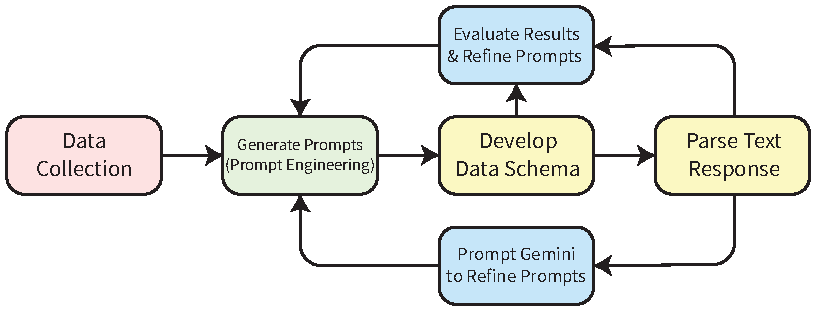
\includegraphics[scale=1,trim={0 0 0 0},clip]{pef.pdf}
    \caption{Prompt Engineering Process}
    \label{fig:prompt_engineering_process}
\end{figure}

\section{Phase 2: The Decoupled Pipeline Framework}\label{ch:3.2}
The limitations identified in the initial study—including high computational cost, lack of quantifiable similarity scores, and prompt sensitivity—directly motivated a pivot to a more sophisticated, decoupled pipeline. This new approach was first developed and prototyped using the initial, manually-curated dataset. This section details this final, more robust methodology, beginning with the larger and more comprehensive data corpus upon which it was ultimately trained and validated.

\subsection{The PPM Corpus and Data Preparation}\label{ch:3.2.1}
The limitations of the initial study necessitated not only a more sophisticated methodology but also a larger, more comprehensive dataset to robustly train and evaluate it. This required data corpus was procured at a later stage of the research in partnership with the Program Pathways Mapper (PPM). The acquisition of this dataset was a critical step that enabled the full-scale implementation and validation of the decoupled pipeline.

The corpus provided by the PPM initially contained 2,217 courses, each labeled with a Course Identification Numbering System (C-ID) code that serves as the ground truth for course equivalency. To prepare this data for a robust, stratified partitioning, a critical filtering step was applied first. All C-ID classes with fewer than four associated courses were removed from the dataset. This step was essential to guarantee that after splitting the data, both the training and subsequent test sets would contain enough examples to form at least one equivalent course pair for every class, a necessary condition for the fine-tuning process. This filtering resulted in a final, clean corpus of 2,157 courses distributed across 157 distinct C-ID classes.

To ensure a rigorous and unbiased evaluation of the final models, this final dataset was partitioned into two distinct, non-overlapping subsets: a training set and a test set. A stratified 50/50 split was employed, using the C-ID code as the stratification key. This resulted in a training set of 1,078 courses and a test set of 1,079 courses. The stratification ensures that each of the 157 classes is represented in both subsets. The test set is held in reserve and used only once for the final, conclusive evaluation of the optimized classification pipeline, providing an honest estimate of the model's generalization performance on unseen data.

\subsection{Input Document Normalization}\label{ch:3.2.2}
In a departure from conventional NLP pipelines, this research deliberately eschewed standard text pre-processing techniques such as lowercasing, stop-word removal, or the stripping of special characters. This decision was made to more accurately simulate a real-world use case where input data may be imperfectly formatted. The methodology, therefore, relies on the inherent semantic power and robustness of modern transformer-based embedding models to interpret and handle this ``raw'' text.

Instead of cleaning the text, a normalization step was performed to create a consistent, structured input document for the embedding models. A new field, ``Formatted Course Info,'' was generated for each course by concatenating four key pieces of information: the department name, the department course number, the course title, and the full course description. This concatenated string serves as the single document representation for each course and is the direct input for the document embedding process, ensuring all relevant textual context is preserved in a standardized format.

\subsection{Feature Engineering}\label{ch:3.2.3}
The high-dimensional embedding vectors generated by the models, while semantically rich, are not the final features used for classification. To prepare the data for the downstream classifiers, a two-stage feature engineering pipeline was executed. This pipeline first applies various dimensionality reduction techniques and then constructs pairwise difference vectors from these embeddings to explicitly represent the relationship between two courses.

\subsubsection{Dimensionality Reduction}\label{ch:3.2.3.1}
The high-dimensional vectors produced by modern embedding models can present challenges for downstream machine learning algorithms, a phenomenon often referred to as the ``curse of dimensionality.'' To address these potential issues, a systematic process of dimensionality reduction was applied. This investigation was motivated by several potential benefits, including improving model generalization by removing redundant or noisy dimensions and reducing computational complexity.

To ensure the integrity of the evaluation and prevent any form of data leakage, the reduction models were governed by a strict protocol. Each reduction technique was fit exclusively on the training data. The same fitted model was then used to transform both the training and the held-out test sets. This methodology guarantees that no information from the test set influences the parameters of the reduction models. A comprehensive exploration was conducted to determine the optimal dimensionality, including using Principal Component Analysis (PCA) to reduce vectors to the number of components required to explain 70\%, 80\%, and 90\% of the original variance, as well as reducing to static 4 and 7 dimensions using PCA, t-SNE, and PaCMAP.

\subsubsection{Composite Distance Vector}\label{ch:3.2.3.2}
The ultimate goal of this research is to classify pairs of courses, which requires input features that represent the relationship between them. To provide a richer, more discriminative representation than a single metric alone, we designed a composite feature vector, \(\Delta_c\). The vector is constructed by concatenating the element-wise difference of the two course embedding vectors (\(\mathbf{A}\) and \(\mathbf{B}\)) with their cosine similarity:
\[ \Delta_c = \left(a_1 - b_1, \dots, a_k - b_k, \frac{\mathbf{A}\cdot\mathbf{B}}{\parallel \mathbf{A} \parallel \parallel \mathbf{B} \parallel } \right) \]
where \(\mathbf{A} = (a_1, \dots, a_k) \) and \(\mathbf{B} = (b_1, \dots, b_k) \) are the \(k\)-dimensional embedding vectors for the two courses. This design is powerful because it provides the subsequent classifier with two distinct types of information simultaneously. The element-wise difference captures granular, dimension-specific (local) disparities between the two semantic representations, while the cosine similarity provides a single, normalized measure of their overall (global) alignment in the vector space. A custom \verb|CoursePairGenerator| class, found in the project's codebase, was implemented to systematically generate these feature vectors for all positive and negative pairs across all embedding and reduction variations.

\section{Model Architecture and Training}\label{ch:3.3}
A central hypothesis of this research is that a generic, pre-trained deep embedding model can be adapted to produce highly specialized and semantically rich embeddings for the specific domain of course descriptions. These bespoke embeddings are expected to provide a more discriminative feature representation for downstream classification tasks compared to off-the-shelf models. This section details the architecture, learning objective, and training protocol used to achieve this adaptation through a process of deep metric learning, as well as the downstream classifiers used to evaluate the resulting features.

\subsection{Embedding Models: Selection and Fine-Tuning}\label{ch:3.3.1}
The selection of an appropriate embedding model is a critical first step that influences the entire downstream pipeline. Rather than committing to a single model, this research began with a broad preliminary analysis of a variety of open-source embedding models to identify strong candidates for a more in-depth, comparative study.

\subsubsection{Model Selection}\label{ch:3.3.1.1}
The initial models reviewed, summarized in Table~\ref{tbl:emb_models}, spanned a wide range of parameter sizes and characteristics. To screen these models efficiently, the simple but effective cosine similarity accuracy metric was used: for a given anchor course, a model was considered correct if the cosine similarity to an equivalent course was greater than the similarity to a non-equivalent course. This initial screening revealed that while performance varied, many models achieved high accuracy. Based on these results and a desire to evaluate a representative spectrum of model sizes, three models were selected for the primary analysis:
\begin{itemize}
    \item \verb|BAAI/bge-small-en-v1.5| (BGE): Representing a high-performing small model.
    \item \verb|avsolatorio/GIST-Embedding-v0| (GIST): Representing a medium-sized model.
    \item \verb|nvidia/NV-Embed-v2| (NVE): Representing a large-scale model.
\end{itemize}
At a later stage of the research, \verb|Salesforce/SFR-Embedding-2_R| (SFR) was also included for additional comparison due to its strong performance on public leaderboards. The foundational architecture for all these models is the transformer, which allows them to generate rich, contextual embeddings suitable for feature extraction.
\begin{table}[!tb]
    \captionsetup{skip=5pt}
    \centering
    \caption{Initial Embedding Model Review}
    \label{tbl:emb_models}
    \begin{tabular}{lcccc}
        \toprule
        Model Name                 & Rank$^{*}$ & Params$^{\dagger}$ & Dims & Acc             \\
        \midrule
        GIST-small-Embedding-v0    & 41         & 33                 & 384  & 0.9759          \\
        bge-small-en-v1.5          & 47         & 33                 & 384  & 0.9670          \\
        GIST-Embedding-v0          & 33         & 109                & 768  & 0.9768          \\
        bge-base-en-v1.5           & 35         & 109                & 768  & 0.9732          \\
        gte-base-en-v1.5           & 31         & 137                & 768  & 0.9732          \\
        mxbai-embed-large-v1       & 24         & 335                & 1024 & 0.9759          \\
        gte-large-en-v1.5          & 21         & 434                & 1024 & 0.9777          \\
        multilingual-e5-large-inst & 34         & 560                & 514  & 0.9670          \\
        stella\_en\_1.5B\_v5       & 3          & 1543               & 8192 & 0.9857          \\
        SFR-Embedding-2\_R         & 4          & 7111               & 4096 & \textbf{0.9839} \\
        Agte-Qwen2-7B-instruct     & 5          & 7613               & 3584 & 0.9804          \\
        nvidia/NV-Embed-v2         & 1          & 7851               & 4096 & 0.9831          \\
        \bottomrule
        \multicolumn{4}{p{6cm}}{\scriptsize $^{*}$ Huggingface Overall Leaderboard Rank} \\
        \multicolumn{4}{p{6cm}}{\scriptsize $^{\dagger}$ in Millions}
    \end{tabular}
\end{table}

\subsubsection{Metric Learning with Batch Triplet Loss Functions}\label{ch:3.3.1.2}
To determine if performance could be further improved, the BGE model was subjected to a fine-tuning process using a metric learning approach. Metric learning aims to learn an embedding space where the geometric distance between samples corresponds to their semantic similarity. The concept of Triplet Loss, first introduced in the context of face recognition, has been widely applied to supervised similarity learning~\cite{Yu2020}. It operates on (Anchor, Positive, Negative) triplets. The fundamental goal is to train the embedding function, \(f(x)\), to map inputs into a vector space where the distance between an anchor sample (\(A\)) and a positive sample (\(P\)) is smaller than the distance to a negative sample (\(N\)) from a different class, enforced by a margin, \(\alpha\). The mathematical formulation is given by:
\[ L(A,P,N)=\max(d(f(A),f(P))-d(f(A),f(N))+\alpha,0). \]
Here, \(d\) represents the Euclidean distance. The \(\max()\) component ensures that loss is only incurred for triplets that violate the margin constraint. A naive ``offline'' implementation of Triplet Loss that forms all possible triplets is computationally infeasible. A more effective approach is ``online'' mining, where informative triplets are selected on-the-fly from within each mini-batch. Recognizing that different triplet mining strategies can significantly impact model performance, this research empirically evaluated all four primary batch-based triplet loss implementations available in the sentence-transformers library:
\begin{itemize}
    \item \textbf{BatchAllTripletLoss}: Computes the loss for all valid triplets within a batch. While comprehensive, the learning signal can be diluted by the high number of ``easy'' triplets.
    \item \textbf{BatchSemiHardTripletLoss}: Considers only semi-hard triplets, where the negative sample is more distant than the positive but still violates the margin. This is a common strategy that balances stability and learning effectiveness.
    \item \textbf{BatchHardTripletLoss}: Implements a more aggressive strategy, using the hardest positive and hardest negative for each anchor. This can accelerate convergence but can also be ``temperamental'' and lead to a noisy optimization landscape.
    \item \textbf{BatchHardSoftMarginTripletLoss}: A variation of \verb|BatchHardTripletLoss| that does not require a manually specified margin parameter, simplifying hyperparameter tuning.
\end{itemize}

\subsubsection{Optimization and Training Protocol}\label{ch:3.3.1.3}
The successful fine-tuning of a model with a challenging objective like \verb|BatchHardTripletLoss| is critically dependent on the choice of optimizer and learning rate schedule. The components selected for this research were not chosen in isolation but as parts of a cohesive, synergistic framework designed to ensure stable and effective learning.{\setlength{\emergencystretch}{5em}\par}

The optimization of the model's weights was performed using the \textbf{AdamW} optimizer. AdamW improves upon the standard Adam optimizer by decoupling the weight decay from the gradient update step. This ensures a more stable and effective regularization, which is crucial for preventing the model from overfitting, particularly given the noisy gradients that can arise from hard-negative mining~\cite{loshchilov2019decoupledweightdecayregularization}.

The optimizer was paired with the \verb|CosineAnnealingWarmRestarts| learning rate schedule. This schedule combines two powerful concepts: cosine annealing, which smoothly decays the learning rate following a cosine curve, and ``warm restarts,'' where the rate is periodically reset to its initial maximum~\cite{pytorchcosanneal}. This technique allows the optimizer to escape suboptimal local minima it may have settled into and explore other regions of the complex loss landscape, increasing the likelihood of finding a higher-quality solution~\cite{loshchilovhutter}.

Finally, the data loading and batching strategy was intrinsically linked to the fine-tuning objective. A crucial constraint of the triplet loss functions is that the training data must contain a minimum of two examples for each class label to form a valid (anchor, positive) pair~\cite{sbertLosses}. To mitigate the risk of creating mini-batches that fail this constraint through simple random sampling, this research leveraged the \verb|GroupByLabelBatchSampler| from the \verb|sentence-transformers| library. This sampler ensures that each mini-batch is constructed by grouping samples with the same label, thereby guaranteeing every batch contains the necessary class diversity to form valid and informative triplets for all anchors~\cite{sbertSamplers}.

\subsection{Downstream Classification Models}\label{ch:3.3.2}
To determine the most effective method for classifying the generated pairwise feature vectors, a broad suite of machine learning algorithms was evaluated. The process began with a comprehensive initial evaluation of eight different models to understand which algorithmic families were best suited to the data. This initial suite included:
\begin{itemize}
    \item \textbf{Linear Models (Logistic Regression, Ridge, Lasso)}: To establish a baseline and test for linear separability.
    \item \textbf{Instance-Based Model (k-Nearest Neighbors)}: To probe the local structure and clustering of the feature space.
    \item \textbf{Kernel-Based Model (Support Vector Machine)}: To test for complex, non-linear decision boundaries.
    \item \textbf{Ensemble Model (Random Forest)}: For its robustness and ability to capture complex feature interactions.
    \item \textbf{Probabilistic Models (LDA and QDA)}: To test assumptions about the geometric distribution of the data.
\end{itemize}
Based on the preliminary results from this comprehensive evaluation, four models were selected for the final, in-depth analysis due to their consistently strong performance: K-Nearest Neighbors (KNN), Support Vector Machine (SVM), Random Forest (RF), and XGBoost. XGBoost, a powerful gradient boosting implementation, was added at this stage to include a state-of-the-art boosting algorithm known for its high performance on structured data, ensuring the final comparison was robust and comprehensive.

\section{Evaluation Framework and Metrics}\label{ch:3.4}
A rigorous, multi-stage evaluation framework was designed to systematically narrow down the optimal combination of embedding models, dimensionality reduction techniques, and classifiers, and to provide a comprehensive view of the entire pipeline's performance. This section details the design of that framework, the metrics used to measure performance, and the statistical methods planned for the final analysis.

\subsection{Multi-Stage Evaluation Design}\label{ch:3.4.1}
The evaluation process was designed as a funnel, beginning with a broad preliminary review to efficiently narrow the field of candidates, followed by a more focused and rigorous analysis on the larger, more comprehensive PPM Corpus.

\subsubsection{Stage 1: Initial LLM Feasibility and Benchmark}
The process began with a broad analysis to assess the feasibility of using a Large Language Model for direct classification and to contextualize its performance. This stage, conducted on the Initial Dataset, involved two parts:
\begin{enumerate}
    \item \textbf{Feasibility Study}: The primary evaluation tested Google's Gemini Pro v1.0 across different input data types (full raw text vs. extracted topics) and three classification schemes (binary, 3-way, and 4-way) to understand its capabilities and limitations.
    \item \textbf{Comparative Benchmark}: To contextualize the results, a comparative analysis was conducted against a suite of other prominent open-source LLMs using the same binary classification task.
\end{enumerate}

\subsubsection{Stage 2: Feature Vector Validation (Ablation Study)}\label{ch:3.4.1.1}
A critical ablation study was designed to validate the efficacy of the novel composite distance vector, \(\Delta_c\). This involved training the full suite of initial classifiers on two different versions of the feature set derived from the Initial Dataset: one using the complete composite vector and one using an ablated vector containing only the element-wise differences. By comparing the performance across these two conditions, it was possible to isolate and measure the contribution of the global cosine similarity feature.

\subsubsection{Stage 3: Evaluation During Fine-Tuning}\label{ch:3.4.1.2}
With the larger, more robust PPM dataset, the most promising non-proprietary embedding models were fine-tuned to specialize them for the course equivalency task. To monitor the quality of the learned embeddings during this process, the \verb|BinaryClassificationEvaluator| from the \verb|sentence-transformers| library was employed. At the end of each training epoch, the evaluator was run on binary-labeled course pairs generated from the training set. The primary metric monitored was Average Precision based on cosine similarity, and the model checkpoint that achieved the highest score on these validation pairs was saved as the best model for that fine-tuning run.{\setlength{\emergencystretch}{5em}\par}

\subsubsection{Stage 4: Final Downstream Classifier Evaluation}\label{ch:3.4.1.3}
The final and definitive evaluation was conducted on the held-out test portion of the PPM dataset. This stage used the feature vectors generated from the best-performing embedding models (both the original off-the-shelf versions and the newly fine-tuned versions). These feature sets were then used to train and evaluate the final selection of high-performing classifiers: KNN, Random Forest, SVM, and XGBoost. This ensures an unbiased assessment of the complete pipeline's ability to generalize to new, unseen data. To find the optimal hyperparameters for each classifier, an exhaustive, brute-force hyperparameter grid search was conducted with 5-fold cross-validation.

\subsection{Performance Metrics}\label{ch:3.4.2}
To facilitate a comprehensive and multi-faceted analysis, a suite of standard evaluation metrics was used to assess the various pipeline configurations across two critical dimensions: classification efficacy and computational efficiency.

\subsubsection{Classification Efficacy}\label{ch:3.4.2.1}
The core assessment of classification performance is based on a standard suite of metrics derived from the confusion matrix, which tabulates the counts of True Positives (\(TP\)), True Negatives (\(TN\)), False Positives (\(FP\)), and False Negatives (\(FN\)). While Accuracy, defined as \(\frac{TP + TN}{TP + TN + FP + FN}\), provides a general overview of correctness, it can be insufficient for capturing the nuances of a classifier's behavior. Therefore, this research also evaluates:
\begin{itemize}
    \item \textbf{Precision}: Calculated as \(\frac{TP}{TP + FP}\), this metric measures a model's exactness. High precision indicates that when the model predicts an equivalency, it is likely to be correct.
    \item \textbf{Recall}: Calculated as \(\frac{TP}{TP + FN}\), this metric measures a model's completeness. High recall indicates that the model is effective at identifying the full set of all true equivalencies.
\end{itemize}
The \textbf{\(F_1\)-Score}, the harmonic mean of Precision and Recall (\(2\cdot\frac{Precision\cdot Recall}{Precision + Recall}\)), is used as the primary metric for reporting and comparing the final classification performance. The \(F_1\)-Score provides a single, robust value that balances the trade-off between precision and recall, making it an ideal metric for this task where both avoiding false equivalencies and identifying all true ones are important.

\subsubsection{Efficiency Metrics}\label{ch:3.4.2.2}
Beyond classification efficacy, the practical viability of each pipeline was assessed by measuring its computational efficiency. Both \textbf{Training Time} and \textbf{Inference Time} were systematically captured during the hyperparameter tuning process using the detailed statistics provided by \verb|scikit-learn|'s \verb|GridSearchCV| utility. Training time reflects the resources required to fit a model configuration, offering insight into the cost of experimentation. Inference time, reported by \verb|GridSearchCV| as \verb|score_time|, measures the time required for a trained model to make predictions on new data. For the use case of this research, inference time is considered the more critical efficiency metric, as it directly impacts the system's real-world responsiveness and scalability in a production environment.

\subsection{Statistical Analysis Plan}\label{ch:3.4.3}
To determine if observed differences in mean performance between models were statistically significant, a formal hypothesis testing procedure was planned for the analysis of the held-out test data.
A one-way Analysis of Variance (ANOVA) was planned to first test the null hypothesis that all four finalist classifiers have equal mean \(F_1\)-scores. A statistically significant result would justify a post-hoc analysis to identify which specific pairs of classifiers differ. Prior to this, the assumption of homogeneity of variances would be checked using Levene's Test (with the Brown-Forsythe correction). This test is critical, as a violation of this assumption would make standard post-hoc tests like Tukey's HSD inappropriate. In the event of unequal variances, the Games-Howell post-hoc test was selected for its robustness, as it does not assume equal variances. This ensures a methodologically rigorous comparison.

\section{Misclassification Analysis Methodology}\label{ch:3.5}
While the quantitative evaluation presented in the preceding sections establishes the performance of the pipeline based on aggregate metrics like the \(F_1\)-score, a purely numerical analysis is insufficient for a complete understanding of the system's behavior. High-level metrics are essential for benchmarking and model selection, but they obscure the underlying nature of a model's failures. They quantify what the performance is but fail to explain why and how errors occur. Relying on such metrics alone can be misleading, as they may overestimate a model's robustness while hiding significant, systematic failure modes~\cite{gauthier2022}.

A critical step in the development of reliable and trustworthy AI systems is a thorough and systematic error analysis that moves beyond aggregate scores to diagnose specific weaknesses. This section, therefore, outlines the methodology for a qualitative diagnosis of the system. The objective is to perform a systematic error analysis on the misclassifications produced by the embedding models to understand the root causes of their failures. This investigation follows a two-pronged methodology.

\subsection{Shared Misclassifications Across Models}\label{ch:3.5.1}
To diagnose the source of model errors, it is first necessary to determine whether they are idiosyncratic to individual models or systematic across them. If misclassifications are largely unique to each model, the errors are likely attributable to model-specific factors, such as architectural differences or suboptimal fine-tuning. Conversely, a significant overlap in misclassified pairs across multiple, diverse models would suggest the presence of systematic errors—failures that stem not from the models but from the data itself. Such errors often arise from annotation artifacts, inherent ambiguity in the source text, or insufficient information to support a clear classification, and they represent a fundamental challenge for any model applied to the dataset.

The first prong of the analysis, therefore, examines these systematic error patterns by analyzing the overlap of misclassified course pairs between the different embedding models. This approach, using visualizations such as Venn diagrams and intersection bar charts, helps distinguish between model-specific weaknesses and challenges that are inherent to the dataset itself.

\subsection{Qualitative Case-Based Review}\label{ch:3.5.2}
The second prong of the analysis is a granular, qualitative review of specific false positive and false negative examples drawn from the held-out test and cross-validation reports. This manual, case-based review is a cornerstone of effective error analysis, enabling the identification of specific artifacts and conceptual flaws that quantitative metrics cannot reveal. This is particularly important for understanding failures in complex semantic tasks. For example, it allows for the investigation of challenges in short-text semantic similarity, where a lack of rich context inherently increases ambiguity and the likelihood of spurious matches~\cite{app13063911}.

The overarching goal of this two-pronged methodology is to generate a structured report of the primary error types. This includes identifying and categorizing the root causes of both False Positives (e.g., high topical overlap without true equivalence) and False Negatives (e.g., semantic divergence in descriptions or data quality issues). This diagnostic approach is designed to inform future improvements to the system by revealing where the pipeline is most likely to fail and why.
\chapter{Experimental Setup and Results}
This chapter presents the empirical results that validate the decoupled, deep metric learning framework proposed in Chapter 3. Having detailed the systematic methodology, we now turn to the execution and outcomes of the multi-stage evaluation plan. The central objective of this chapter is to systematically assess the performance of each component of the pipeline---from the choice of embedding model and the impact of fine-tuning to the effects of dimensionality reduction and the selection of a downstream classifier---to identify the optimal configuration for both classification accuracy and computational efficiency.

The analysis is structured to first establish the validity of the core feature engineering approach before proceeding through the comparative stages of the evaluation. The chapter begins by detailing the computational environment, datasets, and formal evaluation metrics used throughout the experiments. It then immediately presents a critical ablation study to validate the efficacy of the novel composite distance vector (\(\Delta_c\)), the cornerstone of the feature representation. With the feature vector's design validated, the chapter then follows the primary evaluation sequence: first, establishing a baseline by assessing the performance of various off-the-shelf embedding models and classifiers; second, quantifying the performance gains achieved through fine-tuning; and third, analyzing the trade-offs between accuracy and efficiency introduced by dimensionality reduction. The chapter culminates in a definitive comparative analysis on the held-out test data, synthesizing all prior findings to identify the single best-performing pipeline configuration. We begin by outlining the experimental setup that forms the foundation for all subsequent results.

\section{Experimental Environment \& Datasets}
\subsection{Computational Environment}
The research presented in this thesis was conducted using a hybrid computational environment, leveraging both cloud-based services for initial language model evaluations and a powerful on-premise high-performance computing (HPC) cluster for the primary, computationally intensive experiments. The initial direct classification tasks described in Section 3.1 were performed using Google's Gemini v1.0, a proprietary cloud-based Large Language Model. All subsequent stages of the research, including model fine-tuning, embedding generation, dimensionality reduction, and the comprehensive downstream classifier evaluations, were executed on San Francisco State University's ``POLARIS'' High Performance Compute Cluster.

The POLARIS cluster provided a robust and flexible environment, running on Rocky Linux 8.9 with the Slurm Workload Manager for job scheduling. The GPU-intensive deep learning tasks, particularly the fine-tuning of the embedding models, were performed on the \verb|gpucluster node|. This node is equipped with two AMD EPYC 9334 CPUs (providing 64 cores and 128 threads), 1 TB of RAM, and is accelerated by four NVIDIA A100 GPUs, each with 80 GB of VRAM and supported by CUDA v12.4. The extensive hyperparameter grid searches for the traditional machine learning classifiers were primarily run on the \verb|cpucluster|, which consists of three nodes, each powered by two AMD EPYC 9534 CPUs (128 cores, 256 threads) and containing 576 GB of RAM. The cluster nodes are interconnected with a high-speed InfiniBand 200 Gb/s network, ensuring efficient data transfer during distributed tasks.

The entire experimental pipeline was implemented in Python, with Jupyter Notebooks serving as the primary environment for rapid prototyping, initial data exploration, and results analysis. The core deep learning components were built using PyTorch, with extensive use of the Hugging Face ecosystem, including the \verb|Transformers|, \verb|Sentence-Transformers|, and \verb|Hub| libraries for model access and training. The classical machine learning experiments were conducted using \verb|scikit-learn| and \verb|XGBoost|. Data manipulation and analysis were handled with \verb|numpy| and \verb|pandas|, while \verb|plotly| was used for visualization and \verb|dill| for object serialization.

\subsection{Datasets}
The evolutionary methodology described in Chapter~\ref{ch:3} was developed and validated using two distinct datasets, each serving a critical purpose at different stages of the research. The use of a smaller, initial dataset for prototyping followed by a larger, more comprehensive corpus for final evaluation is a core component of the experimental design. Table~\ref{tbl:datasets} provides a comparative summary of the key characteristics of both datasets used in this research.
\begin{table}[!tb]
    \captionsetup{skip=5pt}
    \centering
    \caption{Summary of Datasets Used in Evaluation}
    \label{tbl:datasets}
    \resizebox{\columnwidth}{!}{
    \begin{tabular}{p{0.2\textwidth} p{0.4\textwidth} p{0.4\textwidth}}
        \toprule
        \textbf{Characteristic} & \textbf{Initial Dataset} & \textbf{PPM Corpus} \\
        \midrule
        \textbf{Source} & Manually curated via ASSIST  & Program Pathways Mapper (PPM)  \\
        \addlinespace
        \textbf{Purpose} & Preliminary screening, prototyping, and initial classifier evaluation  & Definitive fine-tuning and final pipeline evaluation  \\
        \addlinespace
        \textbf{Ground Truth} & Established articulation agreements  & Course Identification Number (C-ID)  \\
        \addlinespace
        \textbf{Final Size} & 400 course pairs (for evaluation set)  & 2,157 courses (across 157 classes)  \\
        \addlinespace
        \textbf{Partitioning} & Stratified random sample  & Stratified 50/50 train/test split  \\
        \bottomrule
    \end{tabular}
    }
\end{table}
\subsubsection{Initial Dataset}
The first dataset, hereafter referred to as the Initial Dataset, was a manually curated corpus used for the preliminary investigations in Stages 1 and 2 of the evaluation framework. This dataset was constructed from five lower-division courses at San Francisco State University and their established articulation agreements from 63 other California public colleges, sourced via the ASSIST repository. It was used to establish the initial performance baseline with the direct LLM classification approach and to prototype the decoupled pipeline. The final evaluation set for these preliminary stages consisted of a balanced, stratified random sample of 400 course pairs drawn from a larger set of over 11,000 generated pairs.

\subsubsection{PPM Corpus}
The primary and definitive experiments for this thesis were conducted on the PPM Corpus, a larger and more robust dataset provided by the Program Pathways Mapper (PPM). This corpus served as the foundation for the full-scale implementation, fine-tuning, and final validation of the decoupled pipeline (Stages 3 and 4). After a filtering process detailed in Section~\ref{ch:3.2.1}, the final corpus consists of 2,157 courses, each labeled with a Course Identification Number (C-ID) that serves as the ground truth for equivalency. This corpus was partitioned via a stratified 50/50 split into a training set of 1,078 courses and a held-out test set of 1,079 courses. This held-out test set is crucial for methodological rigor and was used only once for the final, conclusive evaluation of the optimized pipelines to provide an honest and unbiased estimate of their generalization performance.

\subsection{Evaluation Metrics}
To facilitate a comprehensive and multi-faceted analysis, a suite of standard evaluation metrics was used to assess the various pipeline configurations. These metrics were chosen to measure performance across two critical dimensions: classification efficacy and computational efficiency, ensuring that the final recommended pipeline is not only accurate but also practical for real-world deployment.

\subsubsection{Classification Efficacy}
The core assessment of classification performance is based on a standard suite of metrics derived from the confusion matrix, which tabulates the counts of True Positives (\(TP\)), True Negatives (\(TN\)), False Positives (\(FP\)), and False Negatives (\(FN\)). Figure~\ref{} provides a visual representation of this structure. By convention throughout this thesis, the true (actual) class labels are organized along the vertical y-axis, and the labels predicted by the model are organized along the horizontal x-axis.  While Accuracy, defined as \(\frac{TP + TN}{TP + TN + FP + FN}\), provides a general overview of correctness, it can be insufficient for capturing the nuances of a classifier's behavior. Therefore, this research also evaluates:
\begin{itemize}
    \item \textbf{Precision}: Calculated as \(\frac{TP}{TP + FP}\), this metric measures a model's exactness. High precision indicates that when the model predicts an equivalency, it is likely to be correct.
    \item \textbf{Recall}: Calculated as \(\frac{TP}{TP + FN}\), this metric measures a model's completeness. High recall indicates that the model is effective at identifying the full set of all true equivalencies.
\end{itemize}
The \(F_1\)-Score, the harmonic mean of Precision and Recall (\(2\cdot\frac{Precision\cdot Recall}{Precision + Recall}\)), is used as the primary metric for reporting and comparing the final classification performance. The \(F_1\)-Score provides a single, robust value that balances the trade-off between precision and recall, making it an ideal metric for this task where both avoiding false equivalencies and identifying all true ones are important.

\subsubsection{Efficiency Metric}
Beyond classification efficacy, the practical viability of each pipeline was assessed by measuring its computational efficiency. Both Training Time and Inference Time were systematically captured during the hyperparameter tuning process using the detailed statistics provided by \verb|scikit-learn| \!\!'s \verb|GridSearchCV| utility. Training time reflects the resources required to fit a model configuration, offering insight into the cost of experimentation. Inference time, reported by \verb|GridSearchCV| as \verb|score_time|, measures the time required for a trained model to make predictions on new data. For the use case of this research, inference time is considered the more critical efficiency metric, as it directly impacts the system's real-world responsiveness and scalability in a production environment. Finally, for the specific task of monitoring model improvement during the fine-tuning process (Stage 3), a specialized metric, Average Precision based on cosine similarity, was employed by the \verb|BinaryClassificationEvaluator| to select the best-performing model checkpoint.

\section{Direct LLM Classification}
The initial phase of this research sought to establish a performance baseline by evaluating the feasibility of using a Large Language Model for end-to-end course equivalency classification. The experiments were conducted using the Initial Dataset, a balanced 400-pair sample, and leveraged Google's Gemini Pro v1.0 as the reasoning engine. The evaluation was designed to test two key conditions: the impact of input data type (full raw text vs.\ extracted topics) and the effect of different classification schemes (binary, 3-way, and 4-way) on the model's performance and behavior.

The classification results were encouraging, with the model achieving a peak accuracy of 90.5\% in the binary task using raw text. A primary finding from this phase was that using the full, unprocessed raw text consistently yielded superior results compared to using only the extracted structured topics. This performance gap is likely attributable to the challenges inherent in the data extraction step itself. The process of deducing structured topics from unstructured text proved to be the most time-consuming and difficult aspect of this initial approach, requiring two to four times more time than the classification task and exhibiting a high sensitivity to prompt wording—a finding that aligns with previous studies on prompt engineering by Sclar et al., Errica et al., Chen et al., Cheung, and Gerych et al.~\cite{Sclar2023QuantifyingLM,Errica2024WhatDI,Chen2024LLMAA,Cheung2024ARC,Gerych2024WhoKT}. Although Gemini demonstrated a general capability to understand the context of the course descriptions, its limitations in flawlessly deducing course topics appear to have introduced enough noise to degrade the performance of the topics-based classification.

An analysis of the confusion matrices, presented in Figure~\ref{fig:cm} reveals a consistent and telling behavioral pattern: the model exhibits a strong conservative bias. Across all scenarios, the ``not equivalent'' class showed higher recall than precision, while the ``equivalent'' class showed higher precision than recall. For example, in the binary raw text evaluation, the model produced 34 false negatives but only 4 false positives. This indicates that the model is far more likely to misclassify a truly equivalent course as ``not equivalent'' than it is to incorrectly approve a non-equivalent pair. This conservative tendency suggests the LLM operates with a high internal threshold for declaring equivalency, preferring to err on the side of caution.
\begin{figure}[tb]
    \centering
    \begin{subfigure}[b]{0.45\textwidth}
        \centering
        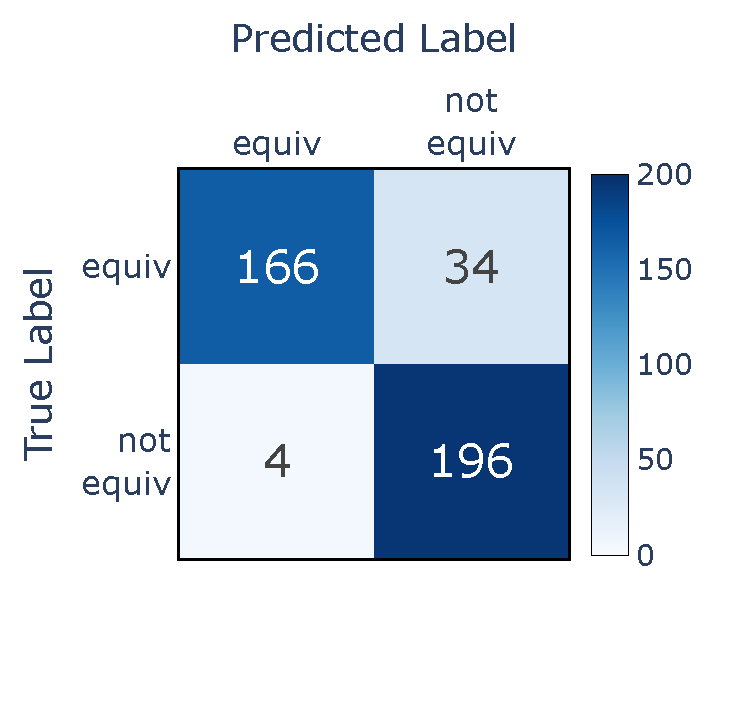
\includegraphics[scale=0.41,trim={3mm 20mm 7mm 0},clip]{LLMeval_binary_raw_text_cm.pdf}
        \caption{Binary Raw Text}
        \label{fig:sub_brt}
    \end{subfigure}
    \hfill
    \begin{subfigure}[b]{0.45\textwidth}
        \centering
        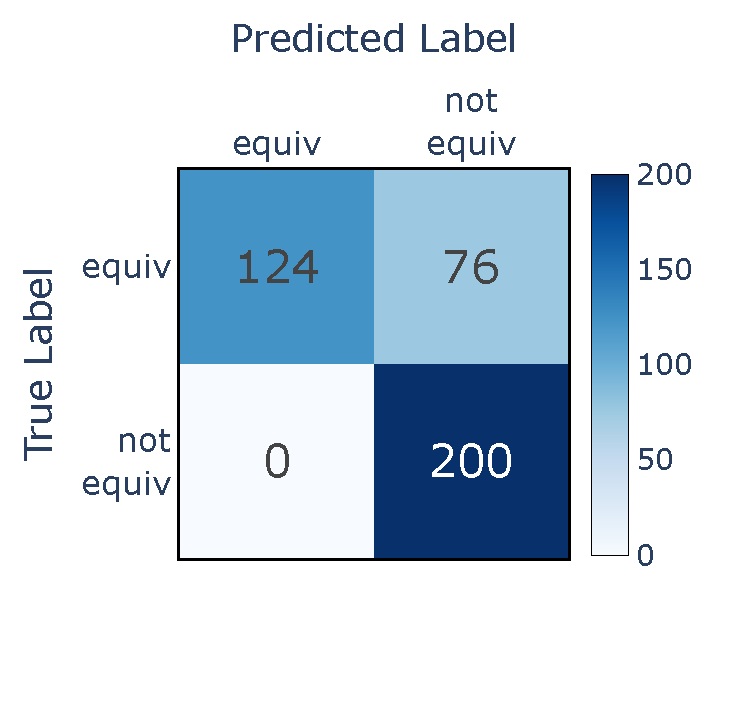
\includegraphics[scale=0.41,trim={3mm 20mm 7mm 0},clip]{LLMeval_binary_topics_cm.pdf}
        \caption{Binary Topics}
        \label{fig:sub_brt}
    \end{subfigure}

    \vspace{2mm}

    \begin{subfigure}[b]{0.45\textwidth}
        \centering
        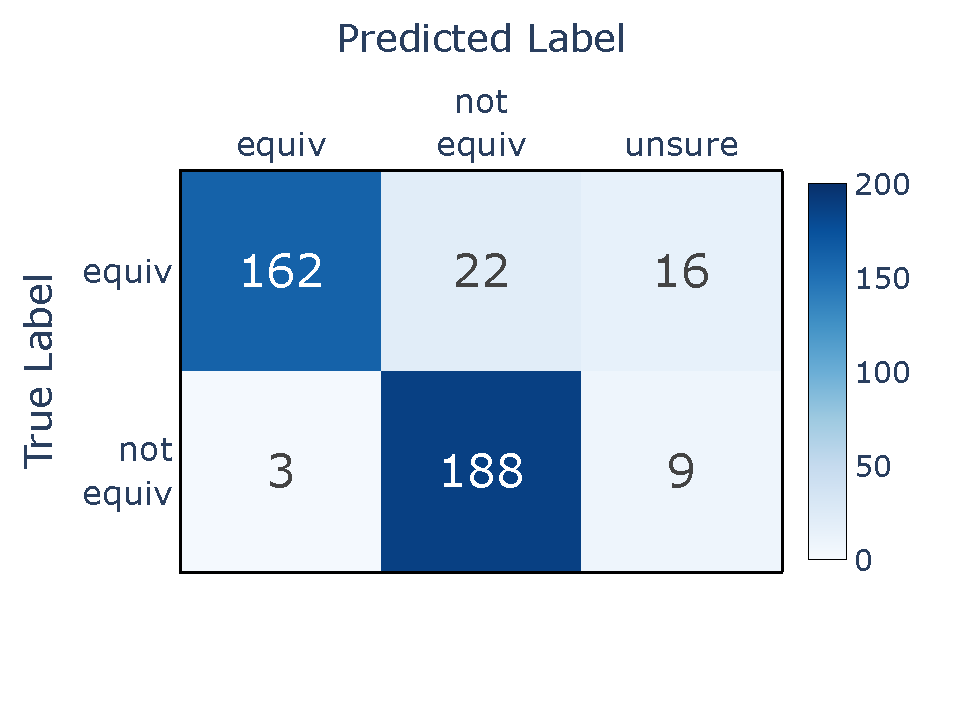
\includegraphics[scale=0.41,trim={3mm 20mm 7mm 0},clip]{LLMeval_3way_raw_text_cm.pdf}
        \caption{3-way Raw Text}
        \label{fig:sub_brt}
    \end{subfigure}
    \hfill
    \begin{subfigure}[b]{0.45\textwidth}
        \centering
        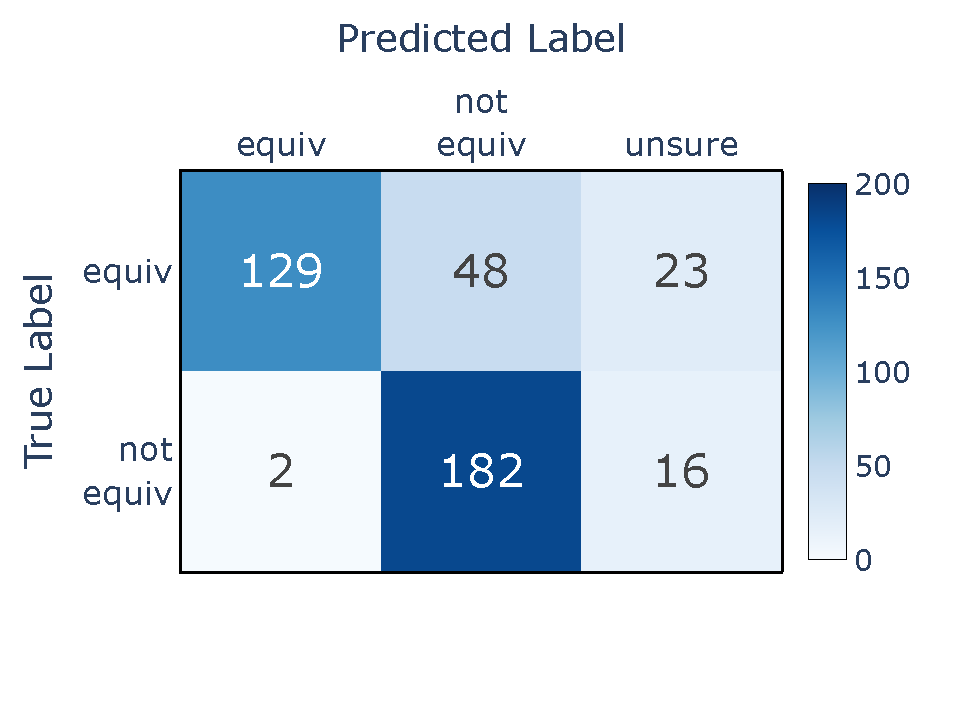
\includegraphics[scale=0.41,trim={3mm 20mm 7mm 0},clip]{LLMeval_3way_topics_cm.pdf}
        \caption{3-way Topics}
        \label{fig:sub_brt}
    \end{subfigure}

    \vspace{2mm}

    \begin{subfigure}[b]{0.45\textwidth}
        \centering
        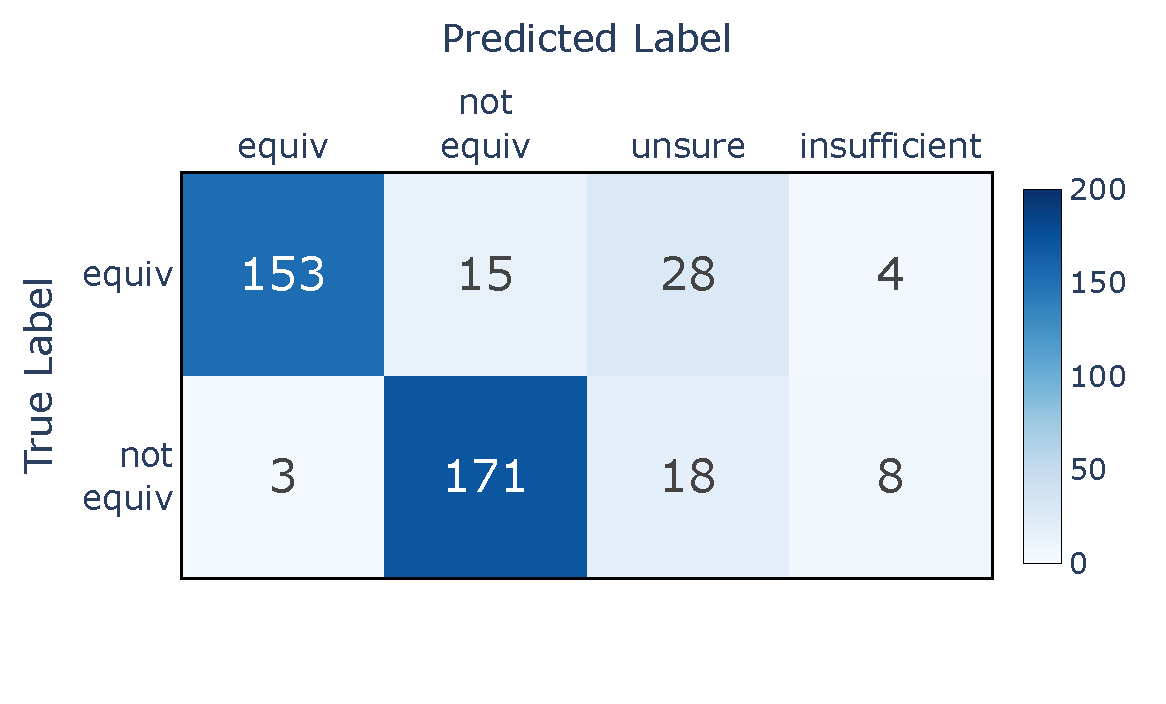
\includegraphics[scale=0.41,trim={3mm 20mm 7mm 0},clip]{LLMeval_4way_raw_text_cm.pdf}
        \caption{4-way Raw Text}
        \label{fig:sub_brt}
    \end{subfigure}
    \hfill
    \begin{subfigure}[b]{0.45\textwidth}
        \centering
        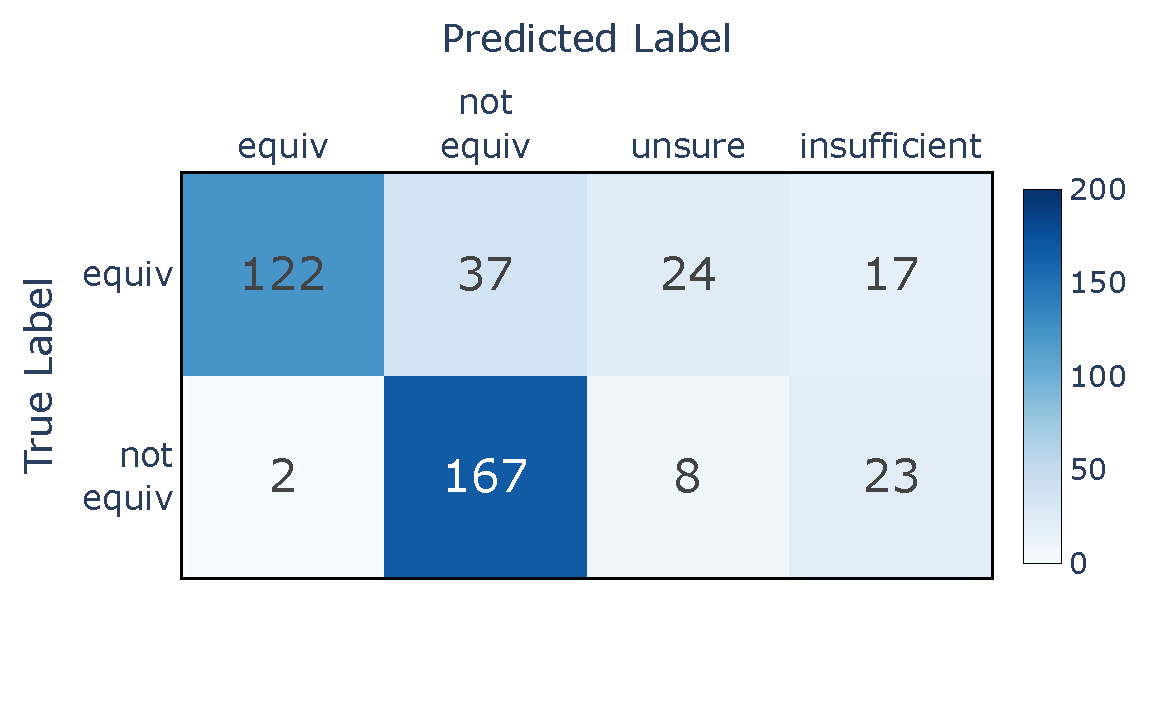
\includegraphics[scale=0.41,trim={3mm 20mm 7mm 0},clip]{LLMeval_4way_topics_cm.pdf}
        \caption{4-way Topics}
        \label{fig:sub_brt}
    \end{subfigure}
    \vspace{-2em}
    \caption{LLM Classification Confusion Matrices}
    % {\footnotesize Clockwise from bottom left: 4-class raw text, 3-class raw text, binary raw text, binary
    %     structured topics, 3-class structured topics, and 4-class structured topics.\\\footnotemark[1]ins: insufficient description}
    \label{fig:cm}
\end{figure}

The introduction of the ``unsure'' and ``insufficient data'' categories was designed to simulate how a human advisor might handle ambiguity. While there is no ground truth for these labels, their value lies in the model's ability to isolate cases that require further manual review. This is particularly relevant for courses that may have significant topical overlap but different learning outcomes, or for descriptions that are too sparse to allow for a definitive decision. For instance, in the 4-way raw text evaluation, the model flagged 46 pairs as ``unsure'' and 12 as having ``insufficient'' information, effectively separating these ambiguous cases from the main classification flow.  Table~\ref{tbl:llm_results_summary} provides a comprehensive summary of the performance metrics for all six experimental conditions.
\begin{table}[!tb]
    \captionsetup{skip=5pt}
    \centering
    \caption{Performance Summary of Direct LLM Classification}
    \label{tbl:llm_results_summary}
    \begin{tabular}{lccccc}
        \toprule
        & \textbf{Classification} & & & & \\
        \textbf{Input Data} & \textbf{Task} & \textbf{Accuracy} & \textbf{F1-Score*} & \textbf{Precision*} & \textbf{Recall*} \\
        \midrule
        \multirow{3}{*}{Raw Text} & Binary & 0.9050 & 0.8973 & 0.9765 & 0.8300 \\
        & 3-way & 0.8750 & 0.8877 & 0.9818 & 0.8100 \\
        & 4-way & 0.8100 & 0.8596 & 0.9808 & 0.7650 \\
        \midrule
        \multirow{3}{*}{Topics} & Binary & 0.8100 & 0.7654 & 1.0000 & 0.6200 \\
        & 3-way & 0.7775 & 0.7795 & 0.9847 & 0.6450 \\
        & 4-way & 0.7225 & 0.7531 & 0.9839 & 0.6100 \\
        \bottomrule
        \multicolumn{6}{p{0.9\textwidth}}{\scriptsize * F1-Score, Precision, and Recall are reported for the positive class (``Equivalent'').} \\
    \end{tabular}
\end{table}

To contextualize the performance of Gemini Pro, a comparative analysis was conducted against a suite of other prominent open-source LLMs (see Table~\ref{tbl:cls} for a summary of their specifications and performance). The results of this benchmark revealed that Gemini Pro v1.0 outperformed all other models tested. While most models were able to complete the task, their performance varied significantly. The strongest competitor was Anthracite Magnum v1 72B, which achieved a respectable accuracy of 85.25\%, but still falling short of Gemini's 90.5\%.
\begin{table*}[tb]
    \captionsetup{skip=5pt}
    \caption{Model Specifications and Performance}
    \label{tbl:cls}
    \centering
    \resizebox{\columnwidth}{!}{
    \begin{tabular}{lccccccc}
        \toprule
        &  & \textbf{Context} &  &  &
                     &      &      \\
        \textbf{Model Name}             & \textbf{Parameters*} & \textbf{Length} & \textbf{Support} & \textbf{Accuracy} &
        \textbf{Precision}              & \textbf{Recall}      & \(\mathbf{F_1}\)\textbf{-score}                                                                                                \\
        \midrule
        Google Gemini Pro 1.0           & Unknown              & 32,768                  & 400              & \textbf{0.9050}   & 0.9765 & \textbf{0.8300} & \textbf{0.8973} \\
        Meta Llama 3.1 8B Instruct      & 8                    & 128,000                 & 208 (52\%)       & 0.6250            & 1.0000 & 0.3500          & 0.5185          \\
        Microsoft Phi 3 Medium Instruct & 14                   & 128,000                 & 400              & 0.7100            & 1.0000 & 0.4200          & 0.5915          \\
        Google Gemma 2 27b              & 27.2                 & 8,000                   & N/A              & N/A               & N/A    & N/A             & N/A             \\
        Meta Llama 3.1 70B Instruct     & 70                   & 128,000                 & 400              & 0.7350            & 1.0000 & 0.4700          & 0.6395          \\
        Qwen 2 72B Instruct             & 72.7                 & 131,072                 & 400              & 0.7650            & 1.0000 & 0.5300          & 0.6928          \\
        Anthracite Magnum v1 72B        & 72.7                 & 32,768                  & 400              & 0.8525            & 1.0000 & 0.7050          & 0.8270          \\
        CalmeRys 78B Orpo v0.1          & 78                   & 32,768                  & 400              & 0.7175            & 1.0000 & 0.4350          & 0.6063          \\
        Mixtral 8x22B Instruct v0.1     & 141                  & 65,536                  & 400              & 0.6450            & 1.0000 & 0.2900          & 0.4496          \\
        Meta Llama 3.1 405B Instruct**  & 405                  & 128,000                 & 400              & 0.7775            & 1.0000 & 0.5550          & 0.7138          \\
        \bottomrule
        \multicolumn{8}{l}{\footnotesize *in Billions}                                                                                                                       \\
        \multicolumn{8}{l}{\footnotesize **INT4 Quantized Model}
    \end{tabular}
    }
\end{table*}

This benchmark also highlighted significant operational challenges. Several models struggled to reliably produce valid output. For example, Google's Gemma 2 27B consistently generated unintelligible or irrelevant responses, preventing the collection of any meaningful performance data. Similarly, Meta's Llama 3.1 8B Instruct model was only able to respond correctly to approximately 52\% of the prompts, making it too unreliable for practical use. A surprising insight from this analysis was the lack of a strong correlation between model size and performance on this task. It is important to note, however, that the prompts used in this evaluation were originally designed and optimized for Gemini. This lack of prompt specificity for the other models may have contributed to their lower accuracy and, in some cases, their inability to respond appropriately.

This initial study confirmed that direct LLM classification can achieve high accuracy but is sensitive to input quality and exhibits a conservative bias. More importantly, it validated the fundamental limitations of the approach, its computational cost, lack of a quantifiable similarity score, and ``black box'' nature, that motivated the development of the decoupled pipeline. The following sections will now present the results of this more advanced framework, beginning with a critical validation of its most novel component: the composite distance vector.

\section{Composite Distance Vector Validation}

\section{Off-the-Shelf Embedding Models}

\section{Fine-Tuned Embeddings Models}

\section{Dimensionality Reduction}

\section{Comparative Analysis}

\section{Summary}
\chapter{Discussion, Future Work, and Conclusion}
This chapter transitions from the empirical validation of the proposed framework to a broader discussion of its implications. Having systematically evaluated each component and demonstrated the model's high performance in Chapter 4, this chapter now seeks to interpret the significance of these results in the context of the course articulation problem. The objective is to discuss the key findings, acknowledge the inherent limitations of the study, and outline promising avenues for future research that build upon this work. The chapter will culminate in a final conclusion, summarizing the primary contributions of the thesis and reiterating its significance for fostering a more equitable and efficient higher education ecosystem.

\section{Discussion of Results}\label{ch:5.1}
The empirical results presented in Chapter 4 offer a robust validation of the core hypothesis of this thesis: that a decoupled, deep metric learning framework can overcome the limitations of prior automated approaches to course articulation. This section discusses the significance of these findings, focusing on the vindication of the proposed framework, the critical impact of domain-specific fine-tuning, and the resulting shift in focus from model-centric to data-centric challenges.

\subsection{A Vindicated Framework}\label{ch:5.1.1}
The proposed pipeline successfully addresses the distinct challenges that have hindered previous attempts at automation. By relying exclusively on publicly available course catalog data, the framework is an inherently privacy-preserving alternative to enrollment-based methods like \emph{course2vec}, which are constrained by their need for sensitive, proprietary student records and are not generalizable to institutions with no prior transfer history~\cite{pardos2018connectionistrecommendationwildutility, slade10.1177/0002764213479366}. Furthermore, by decoupling semantic representation from classification, the framework is significantly more scalable, efficient, and interpretable than using large language models for direct, end-to-end classification. It avoids the high computational costs, ``black box'' opacity, and prompt sensitivity associated with direct LLM approaches while still providing a quantifiable similarity score for each pair. Finally, its use of deep contextual embeddings represents a fundamental advance over older statistical methods like TF-IDF, which lack any true semantic understanding and cannot grasp synonymous or related concepts~\cite{AIZAWA200345}.

\subsection{The Critical Impact of Domain-Specific Fine-Tuning}\label{ch:5.1.2}
Perhaps the most significant finding from the experimental evaluation is the statistical superiority of the fine-tuned \textbf{bge-ft} model over all off-the-shelf competitors, including those that are orders of magnitude larger. This result provides powerful evidence that for specialized domains, targeted adaptation is more effective than sheer scale. General-purpose models, despite being trained on vast swaths of the internet, lack the specialized ``vocabulary'' to appreciate the fine-grained distinctions in course catalog text. For example, they may not understand the subtle but critical differences between a ``survey'' course, an ``introductory'' course, and a ``foundations'' course. The process of fine-tuning with a triplet loss objective effectively retrained the model's attention mechanism, teaching it the specific semantics and nuances of the academic domain. This allowed it to generate a far more discriminative embedding space, ultimately leading to higher accuracy in the downstream classification task.

\subsection{The Bottleneck Has Shifted from Model-Centric to Data-Centric}\label{ch:5.1.3}
With the optimized pipeline achieving \(F_1\)-scores approaching or exceeding 0.98, the framework has pushed the limits of what can be achieved with the available data. The qualitative misclassification analysis in Section~\ref{ch:4.6} revealed that the vast majority of the remaining errors are not due to failures in the model's semantic understanding. Instead, they are artifacts of the source data itself. The model fails when officially equivalent courses are described with vastly different pedagogical language (semantic divergence) or when descriptions are too vague or minimalist to contain a clear signal. In these cases, the model is performing correctly—it accurately reports that the texts are not semantically similar. The error lies in the ground-truth expectation that an equivalence should be found where none is textually supported.

This leads to a critical insight: the primary bottleneck for achieving near-perfect automation has shifted from being model-centric to data-centric. Simply using a larger or more complex model is unlikely to resolve these data-inherent issues. This suggests that the most promising path to further improvement lies not in novel architectures, but in methodologies that directly address the quality and consistency of the input data~\cite{gauthier2022}, a point that will be explored further in the following sections.

\section{Limitations of the Current Study}\label{ch:5.2}
While the proposed framework represents a significant advance, it is essential to acknowledge the limitations that define the boundaries of the current study. These limitations, primarily rooted in the nature of the data and the scope of the task, provide critical context for the results and inform the directions for future work.

\subsection{Data Quality as a Performance Ceiling}\label{ch:5.2.1}
The primary limitation, as identified in the discussion, is that the framework's performance is fundamentally capped by the quality and content of the public course descriptions. The system can only analyze the text that is provided; it cannot infer information that is absent. As the misclassification analysis demonstrated, when course descriptions are vague, minimalist, or use semantically divergent language to describe functionally equivalent courses, the model's ability to determine a correct match is severely hindered. This reliance on the source text means the system is vulnerable to inconsistencies and information gaps in how institutions write and publish their catalogs.

\subsection{Generalizability of the Fine-Tuned Model}\label{ch:5.2.2}
The \textbf{bge-ft} model was fine-tuned and evaluated on a corpus drawn exclusively from California's public colleges and universities. While the framework itself is general, the specific fine-tuned model has been specialized for the linguistic patterns, terminology, and pedagogical styles common to this system. Its performance may not be as high "out-of-the-box" on data from private institutions or different state systems or non-domestic systems, which may have distinct catalog writing conventions. Achieving similar performance in a new institutional context would likely require re-tuning the model on a sample of local data.

\subsection{Scope of "Equivalency"}\label{ch:5.2.3}
This research operationalizes course equivalency as a function of the semantic similarity of their catalog descriptions. This is a powerful proxy, but it does not encompass the full spectrum of factors that human articulation officers may consider. Decisions made by faculty and administrators can be influenced by factors beyond the written content, such as the rigor of the assessment methods, specific lab equipment, faculty credentials, or overarching institutional agreements. The current model is not designed to capture this external, non-textual context.

\subsection{Handling of Complex Articulation Rules}\label{ch:5.2.4}
The framework simplifies the articulation task into a binary classification of course pairs (equivalent or not-equivalent). This approach does not natively handle the more complex articulation scenarios that exist in practice, such as one-to-many (e.g., one university course is equivalent to two community college courses), many-to-many, or non-symmetrical agreements. While the similarity scores produced by the system could inform the discovery of such relationships, the current classification pipeline is not designed to identify them directly, a challenge that persists for many automated systems~\cite{pardos-articulation-2019}.

\section{Future Work}\label{ch:5.3}
The findings and limitations of this study give rise to several promising avenues for future research. These directions aim to address the remaining challenges by improving the quality of the input data, expanding the framework's capabilities, and exploring more advanced modeling techniques.

Given that data quality was identified as the primary performance bottleneck, the most critical future work involves data-centric strategies. An interactive, human-in-the-loop system could be developed where the model flags ambiguous pairs for an expert reviewer. This system could be further enhanced with dynamic data augmentation; for instance, if a classification falls below a predetermined confidence threshold, the framework could automatically request a more detailed syllabus for the course pair to enable a more informed re-assessment. In addition to manual review, research could explore methods to automatically enrich or standardize course descriptions before analysis, perhaps by using a large language model in a controlled, pre-processing step to create more consistent inputs.

Beyond improving the data, the framework itself can be expanded to be more useful and tunable for institutional needs. In fact, active development is currently underway to evolve the framework beyond binary classification and build a full-scale course recommendation engine, which is currently being actively researched and developed by our team and will provide a conversational interface for a more intuitive user experience. Such a system would use the vector similarity scores to provide students and advisors with a ranked list of the most likely equivalent courses at a target institution. Likewise, Furthermore, future work could investigate the classifier's decision threshold as a mechanism for institutional control, allowing administrators to tune the system's behavior from a more lenient stance to one that errs on the side of caution. To address the limitation of complex articulations, another avenue of research involves modeling curricula as graphs and applying graph neural networks to identify one-to-many and many-to-many relationships.

Finally, there remain opportunities to refine the core machine learning components of the pipeline. Future work could systematically investigate alternative composite distance measures and feature combinations to determine if a more optimal representation exists for the downstream classifiers. This could be complemented by exploring multi-modal learning, extending the model to analyze not just the catalog description but also the full text of course syllabi or textbook lists. Likewise, more room still remains to explore task-optimized loss functions for fine-tuning.  Because the embedding vectors are not being used directly, but as upstream feature engines, creating loss functions that behave more similarly to the downstream classifier may have a significant impact on training efficacy.  As models evolve, more sophisticated training methods, such as instruction-tuning on a small, expert-curated dataset, could also be employed to teach the model the explicit task of explaining course equivalency, potentially yielding more interpretable results.

\section{Conclusion}\label{ch:5.4}
The manual process of determining course equivalency remains a significant impediment to student mobility in higher education, creating administrative burdens and systemic inequities that lead to student credit loss and delayed graduation~\cite{gao2017, collegeopportunity2017}. This thesis confronted this challenge by designing, developing, and validating a novel computational framework that successfully automates course articulation using only publicly available data. The work's primary contribution is a privacy-preserving, scalable, and computationally efficient pipeline that overcomes the limitations of previous automated approaches. This was achieved through two key technical innovations: the application of deep metric learning to fine-tune a bespoke embedding model for the specific semantics of the academic domain, and the design of a novel composite distance vector that provides a richer feature set for downstream classification.

The result of this research is a highly accurate framework, capable of achieving state-of-the-art performance on a real-world dataset. More importantly, it represents a practical tool that institutions can use to reduce administrative workload, provide faster and more consistent guidance to students, and ultimately foster a more transparent and equitable educational ecosystem. By mitigating the barriers faced by transfer students, particularly those from underrepresented backgrounds~\cite{ace2025}, this work contributes a meaningful step toward fulfilling the promise of accessible and efficient pathways through higher education.

\sloppy
\printbibliography
\fussy

\appendix
\addappheadtotoc

\chapter{LLM Prompts}\label{app:llmprompts}
For all prompts \verb|<| and \verb|>| enclose variables. 

\section{Example: Topic Extraction}\label{app:extractionprompt}
Below is a template for the entire prompt used for topic extraction. ``$\langle$'' and ``$\rangle$'' enclose variables.
\begin{lstlisting}
    You are given the task of parsing course information from raw text. This text may be in formats that are hard to read or are incorrectly formatted.  Your task is to correctly separate the course description into its component parts. These parts are the course department code, course number, title, unit count, lecture hours, key topics covered, the appropriate student audience, the prerequisite requirements, and available alternate grading options. Finally, with all the information you are given, deduce the academic discipline that the \textbf{course b}elongs to. Your audience is another expert, so omit terms or words that are irrelevant to the course. The following is the text you are analyzing:
    ```<course description>'''
    
    The output should be formatted as a JSON instance that conforms to the output schema below. As an example, for the schema {``properties": {``foo": {``title": ``Foo", ``description": ``a list of strings", ``type": ``array", ``items": {``type": ``string"}}}, ``required": [``foo"]} the object {``foo": [``bar", ``baz"]} is a well-formatted instance of the schema. The object {``properties": {``foo": [``bar", ``baz"]}} is not well-formatted. Here is the output schema:
    ```<output schema generated by Pydantic>'''
    
    **Consider conjunctions and disjunctions:** Pay attention to conjunctions (e.g., ``and") and disjunctions (e.g., ``or") for all categories. These indicate that multiple conditions may be required, and they should be reflected in the output.
    
    **Be exhaustive:** Ensure that all possible conditions or options are considered and included in the output. Do not exclude any valid options or conditions.
    
    **For the ``student audience category'' field:**
    *   **Identify the target phrase:** Look for phrases like ``Primarily for", ``Intended for", ``Designed for", etc., that indicate the intended student audience.
    *   **Extract relevant terms:**  Once the target phrase is found, extract the subsequent words that describe the student majors or fields of study.
    *   **Exclude unnecessary words:** Filter out any irrelevant words such as ``students", ``majors", ``and", etc., that do not provide specific information about the student audience.
    
    **For the ``alternate grading options'' field:**
    *   **Identify keywords:** Look for keywords such as ``Grades", ``Grading", ``Option", etc., that indicate the presence of alternate grading options.
    *   **Extract options:** Extract the specific grading options mentioned, such as ``P/NP", ``Letter Grade", ``Pass/Fail", etc.
    *   **Exclude unnecessary words:** Similar to the ``students" field, remove unnecessary words like ``options", ``available", etc.
    
    **Do NOT speculate** Ensure that you use ONLY the information provided and do not attempt to infer any information if it is not explicitly provided EXCEPT for the academic discipline.

    Respond only with valid JSON. Do not write an introduction or summary.
\end{lstlisting}

\section{Example: Raw Text Equivalency Evaluation}\label{app:rawequivprompt}

\begin{lstlisting}
    Determine whether the two following courses are equivalent. For course equivalency, respond with <response_type>.

    Course 1:
    ```<target>```

    Course 2:
    ```<source>```

    The output should be formatted as a JSON instance that conforms to the output schema below.

    As an example, for the schema \{"properties": \{"foo": \{"title": "Foo", "description": "a list of strings", "type": "array", "items": \{"type": "string"\}\}\}, "required": \["foo"\]\} the object \{"foo": \["bar", "baz"\]\} is a well-formatted instance of the schema. The object \{"properties": \{"foo": \["bar", "baz"\]\}\} is not well-formatted.

    Here is the output schema:
    ```
    <output schema generated by Pydantic>
    '''

    *Consider conjunctions and disjunctions:**
    Pay attention to conjunctions (e.g., "and") and disjunctions (e.g., "or") for all categories. These indicate that multiple conditions may be required, and they should be reflected in the output.

    **Be exhaustive:** Ensure that all possible conditions or options are considered. Do not exclude any valid options or conditions.
\end{lstlisting}

\section{Example: Topic Equivalency Evaluation}\label{app:topicequivprompt}

\begin{lstlisting}
    User: As an expert course description evaluator you are given the task of determining whether the two following courses are equivalent.
    The course data you are given is separated into categories:
        1. Discipline
        2. Course Title
        3. Topics (formatted as a list)
    The "Target Course" describes the candidate course that the source course may fulfill the requirements for.
    The "Source Course" describes the course that a student has taken that may fulfill the requirements for the target course.

    For course equivalency, respond with 0 if it does not filfill the requirements, 1 if it does fulfill the requirements, 2 if you are unsure, or 3 if there is insufficient data.

    Target Course:
    ```
    1. <target["discipline"]>
    2. <target["title"]>
    3. <target["topics"]>
    ```

    Source Course:
    ```
    1. <source["discipline"]>
    2. <source["title"]>
    3. <source["topics"]>
    ```

    The output should be formatted as a JSON instance that conforms to the output schema below.

    As an example, for the schema \{"properties": \{"foo": \{"title": "Foo", "description": "a list of strings", "type": "array", "items": \{"type": "string"}}}, "required": ["foo"]} the object \{"foo": ["bar", "baz"]} is a well-formatted instance of the schema. The object \{"properties": \{"foo": ["bar", "baz"]}} is not well-formatted.

    Here is the output schema:
    ```
    <output schema generated by Pydantic>
    '''

    *Consider conjunctions and disjunctions:**
    Pay attention to conjunctions (e.g., "and") and disjunctions (e.g., "or") for all categories. These indicate that multiple conditions may be required, and they should be reflected in the output.

    **Be exhaustive:** Ensure that all possible conditions or options are considered. Do not exclude any valid options or conditions.

    **EXAMPLES:**
    EXAMPLE 1:
    Target Course:
        1. Mathematics
        2. Calculus with Analytic Geometry I
        3. ["Calculus", "Analytic Geometry", "Differentiation", "Integration", "Limits", "Curve Sketching", "Applications"]
    Source Course:
        1. Mathematics
        2. Calculus I
        3. ["Calculus", "Differentiation", "Integration", "Transcendental functions"]
    Response: 1

    EXAMPLE 2:
    Target Course:
        1. Computer Science
        2. Programming Concepts and Methodology II
        3. ['Application of object-oriented techniques', 'Program complexity using abstraction', 'Algorithm analysis and Big-O notation', 'Advanced language features', 'Basic sorting and searching algorithms', 'Recursion']
    Source Course:
        1. Computer Science
        2. Introduction to Object-Oriented Programming: Java
        3. ['Object-oriented design', 'Software engineering principles', 'Fundamental programming skills in Java']
    Response: 0
\end{lstlisting}

\chapter{ROC/AUC Curves and Confusion Matrices}\label{app:roc_cm}

\clearpage
\section{ROC/AUC Curves}

\begin{figure}[!h]
    \captionsetup{skip=5pt}
    \centering
    \captionsetup[subfigure]{oneside,margin={1cm,0cm}}
    \subfloat[Zoomed]{
        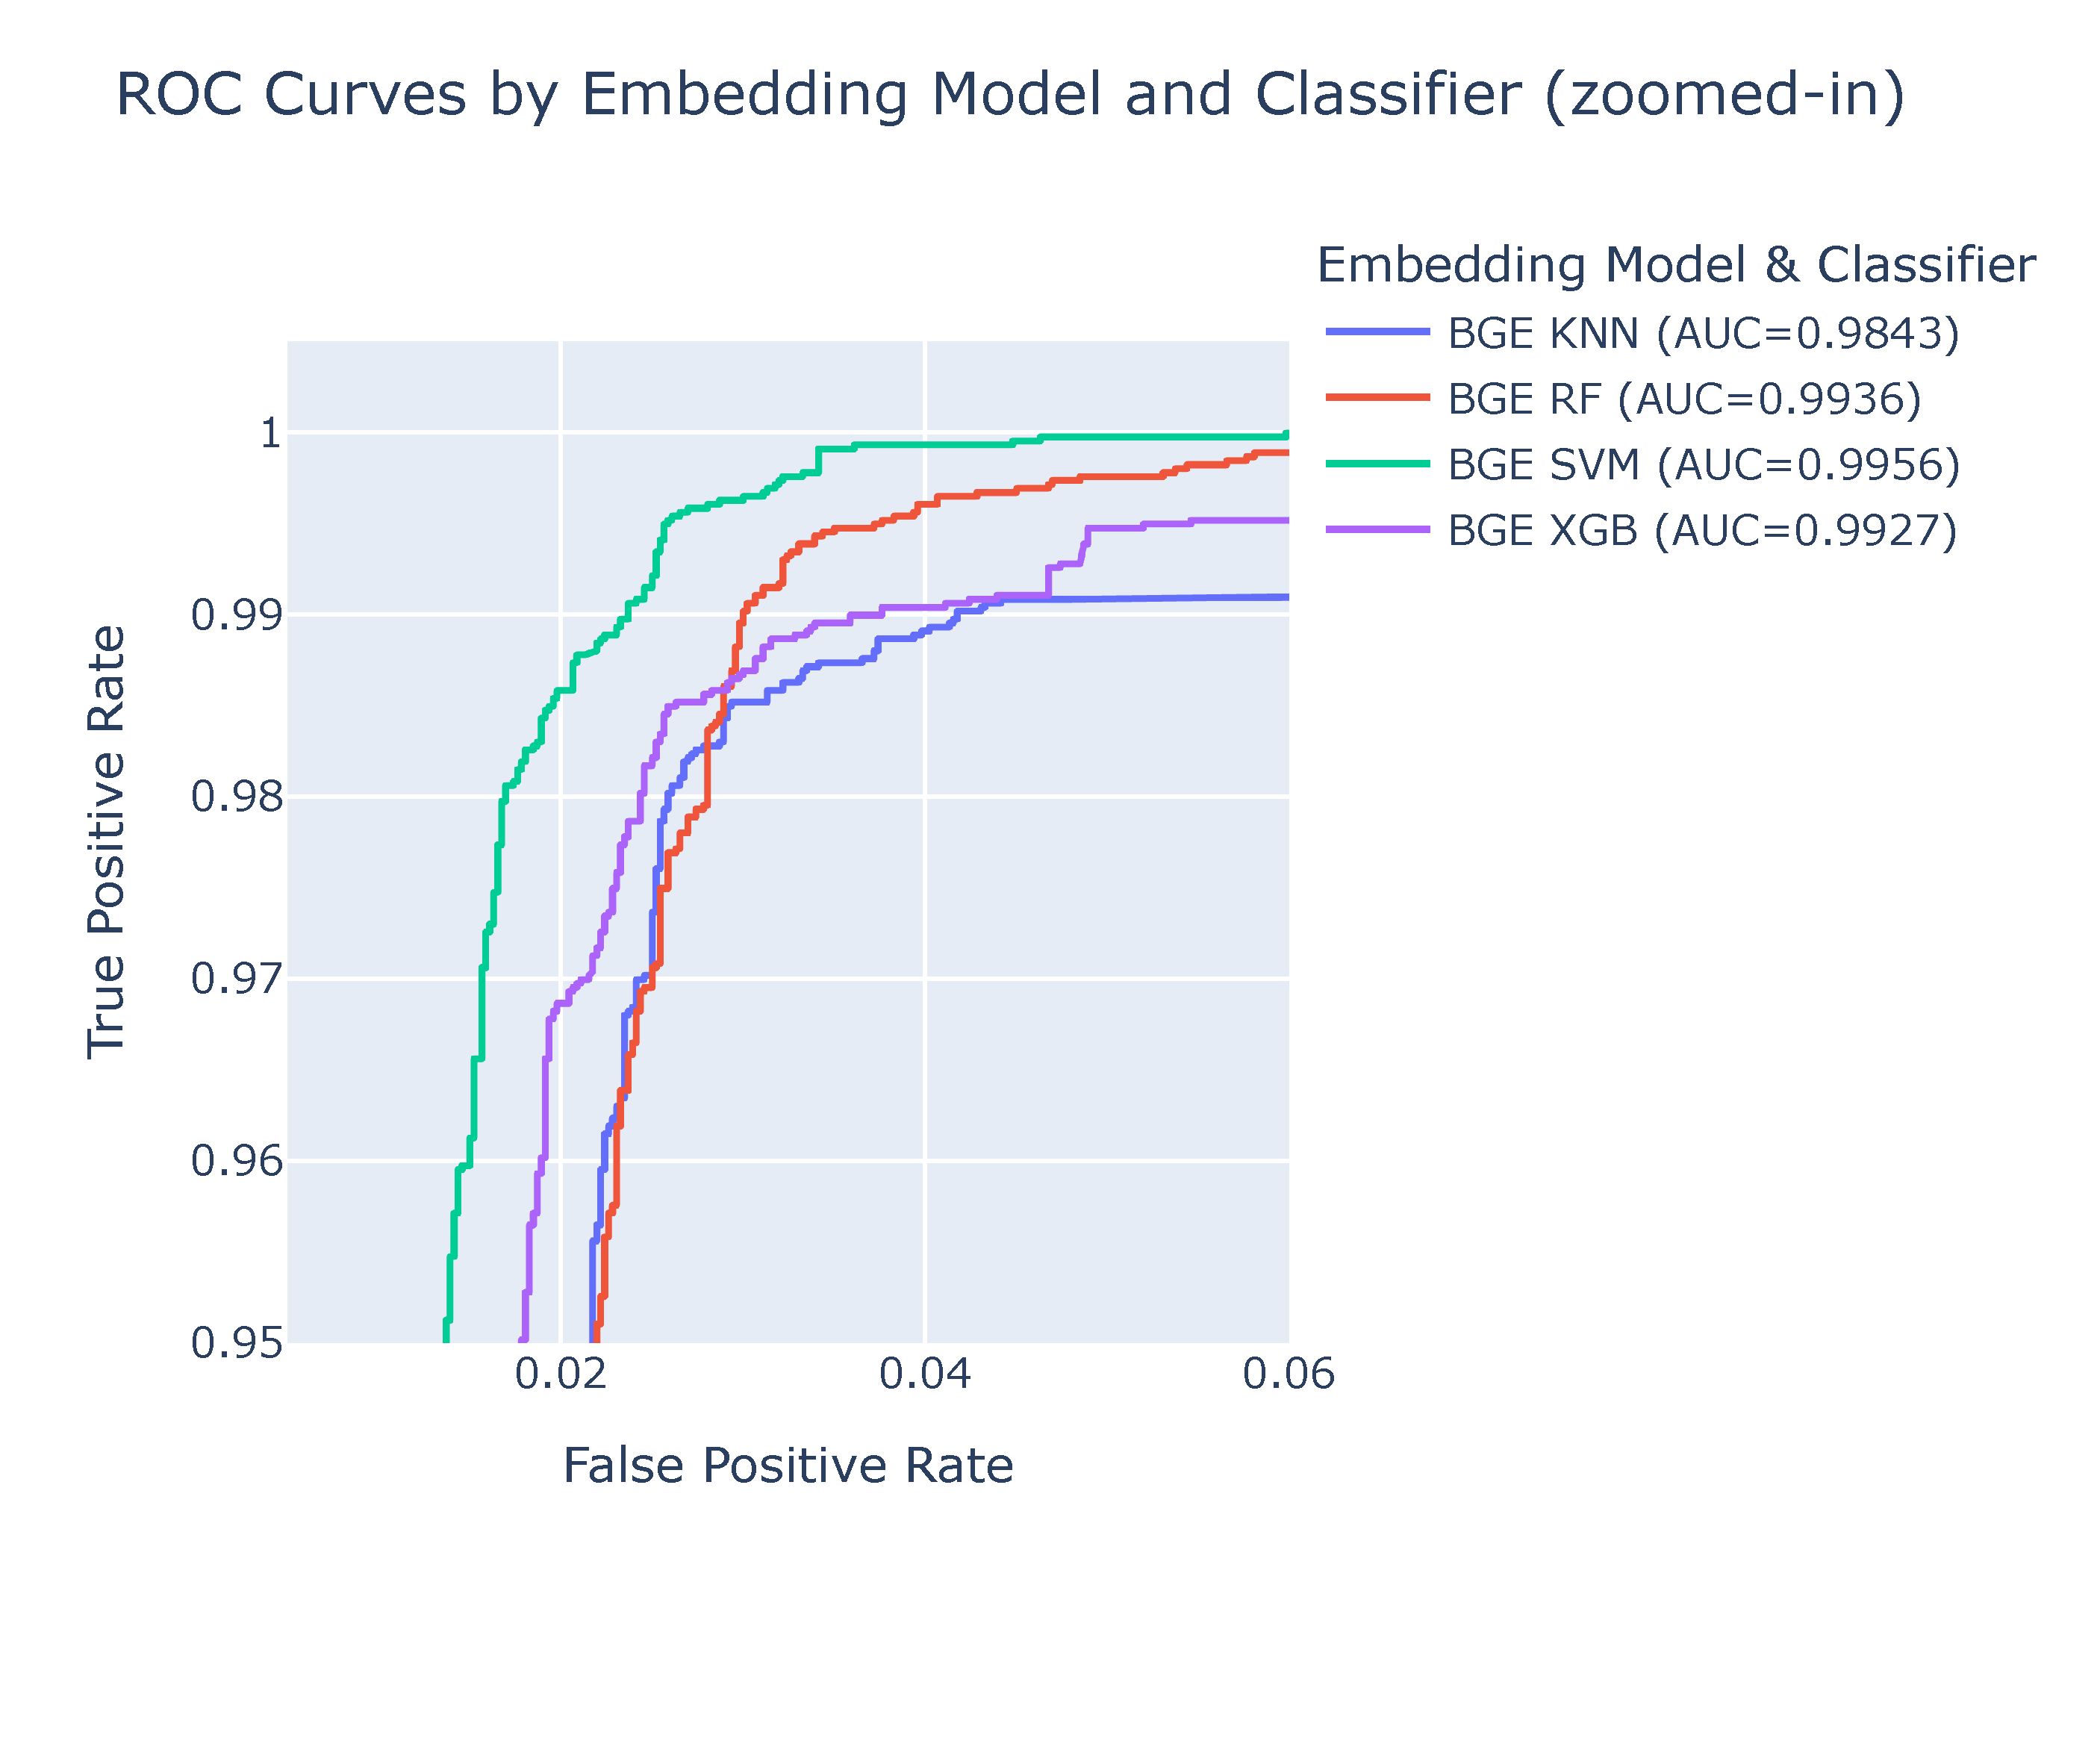
\includegraphics[width=0.37\textwidth,trim={18mm 50mm 180mm 50mm},clip]{roc_curves_bge_zoomed.pdf}\label{fig:bge_roc_zoomed}
    }
    \captionsetup[subfigure]{oneside,margin={-2.5cm,0cm}}
    \subfloat[Full Size]{
        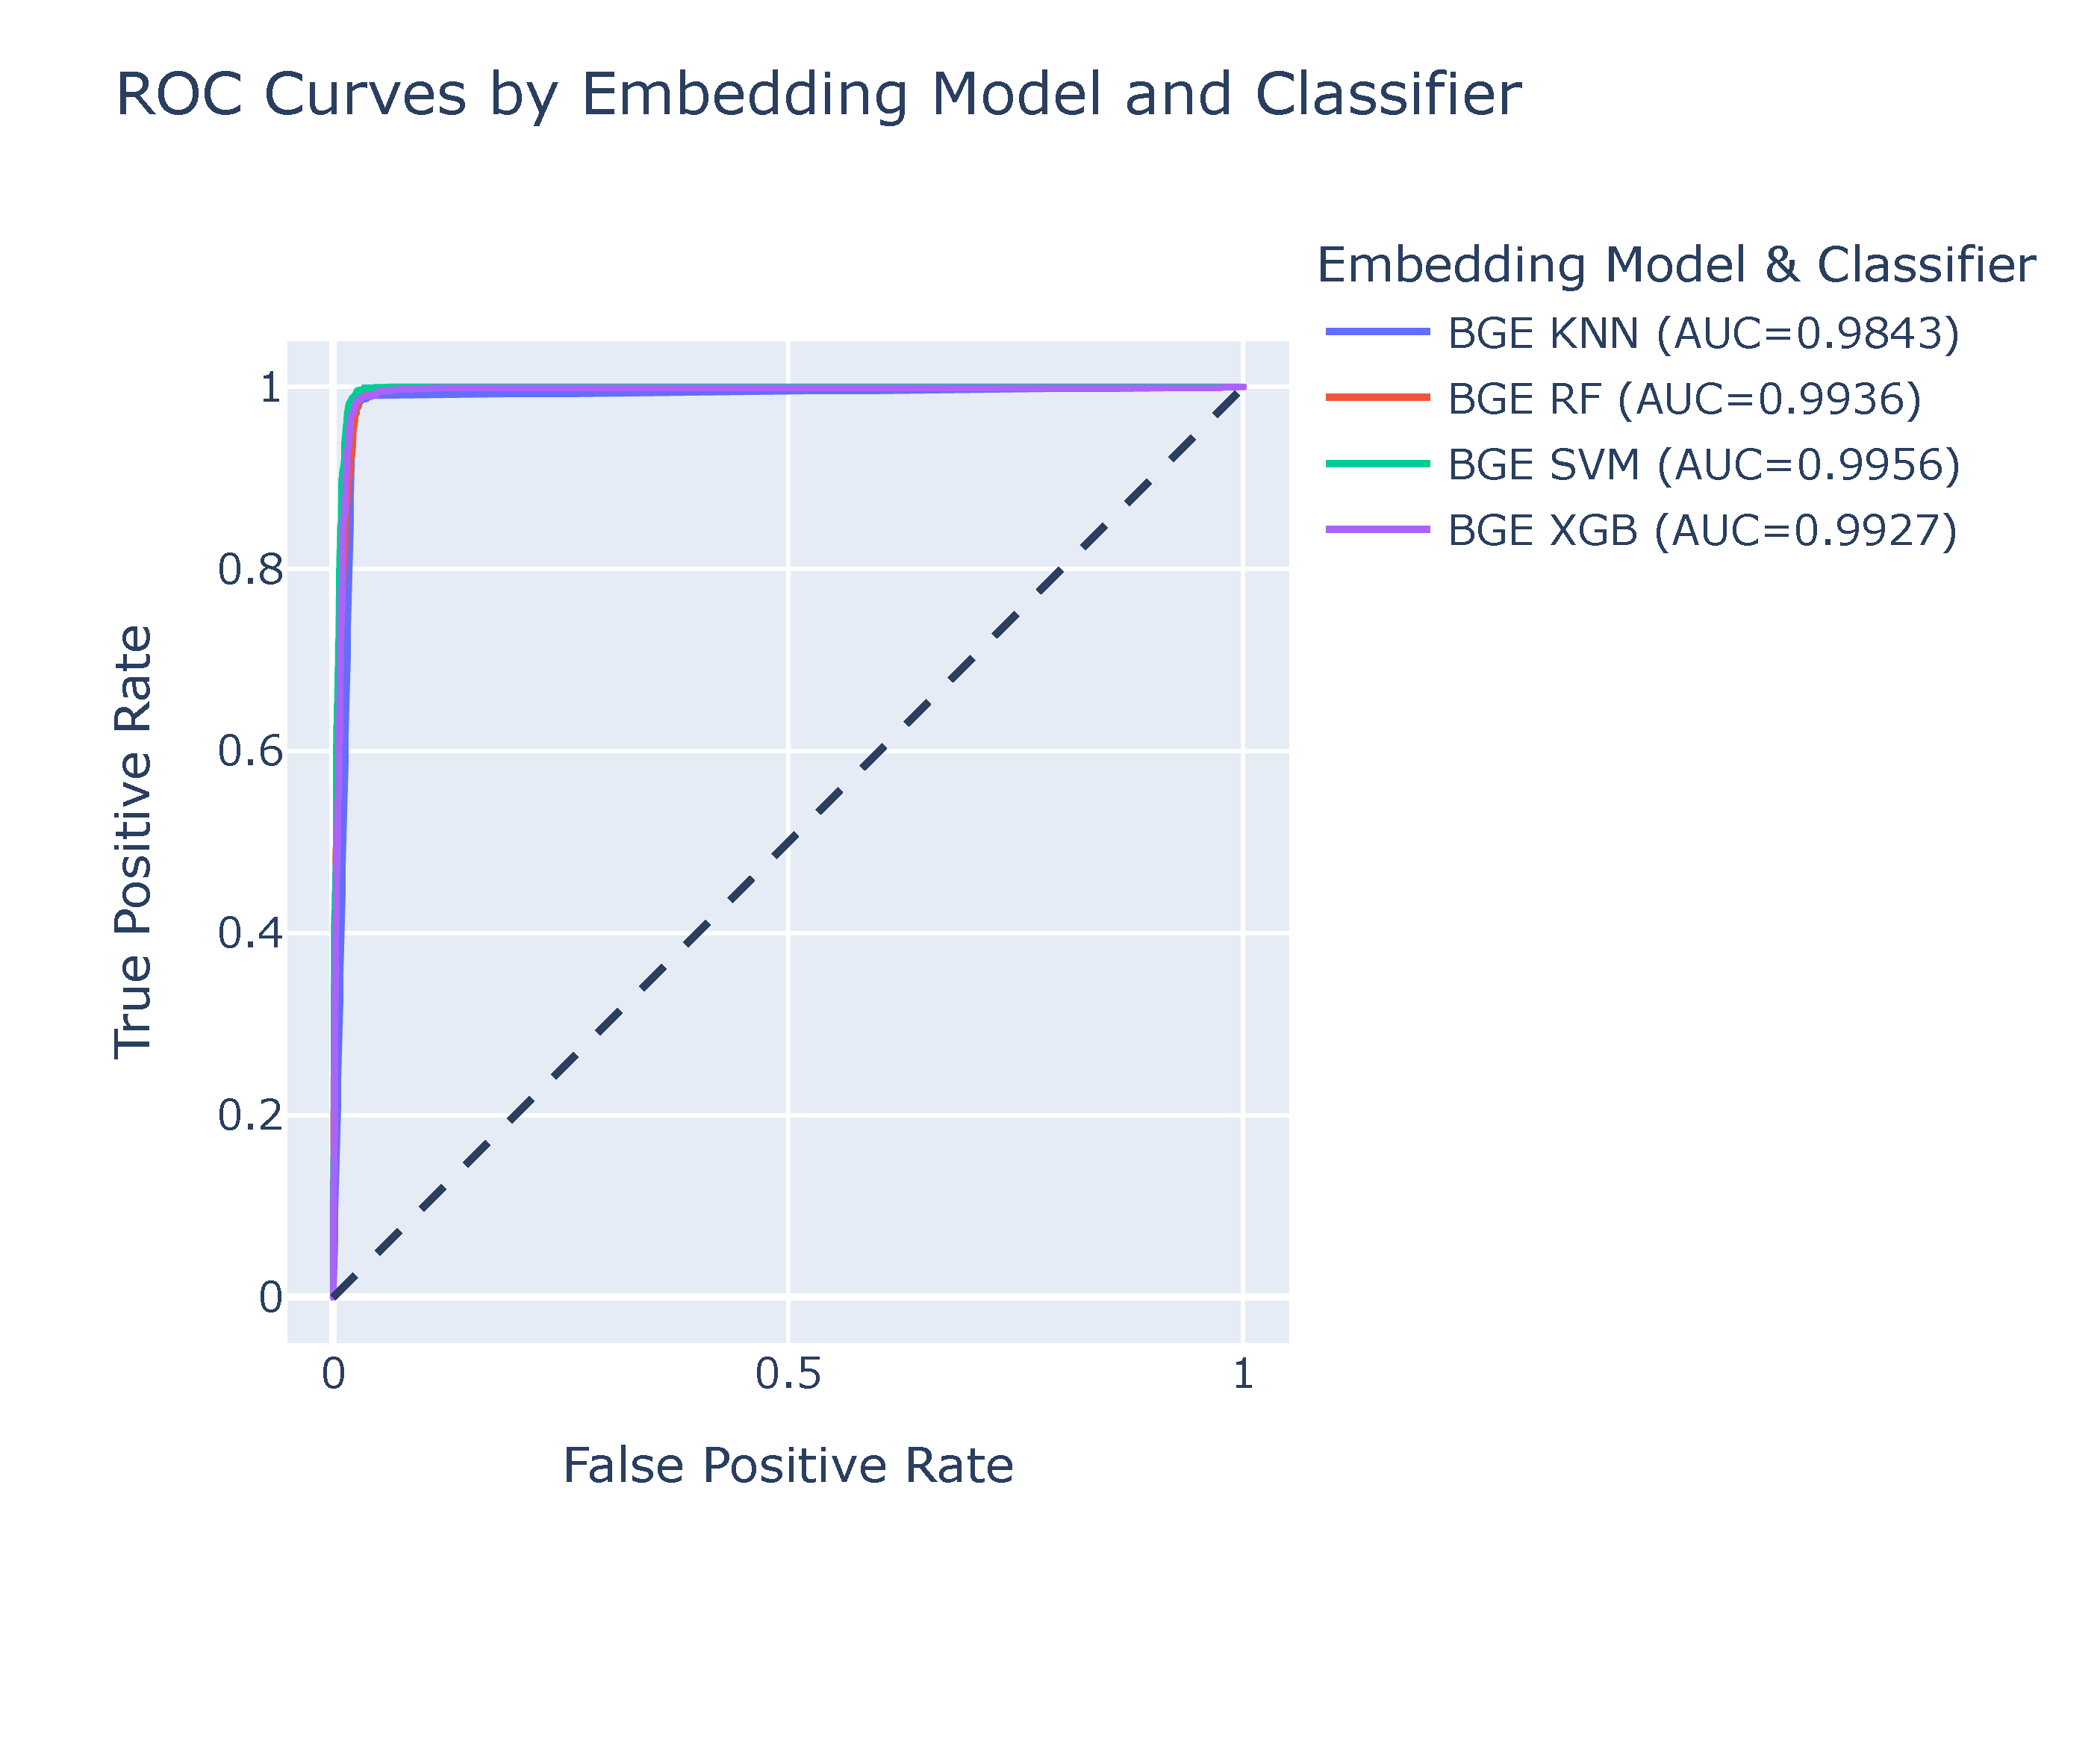
\includegraphics[width=0.58\textwidth,trim={25mm 50mm 12mm 50mm},clip]{roc_curves_bge.pdf}\label{fig:bge_roc_unzoomed}
    }
    \caption{BGE ROC Curves for Finalist Classifiers with Test Data}
\end{figure}

\begin{figure}[!h]
    \captionsetup{skip=5pt}
    \centering
    \captionsetup[subfigure]{oneside,margin={1cm,0cm}}
    \subfloat[Zoomed]{
        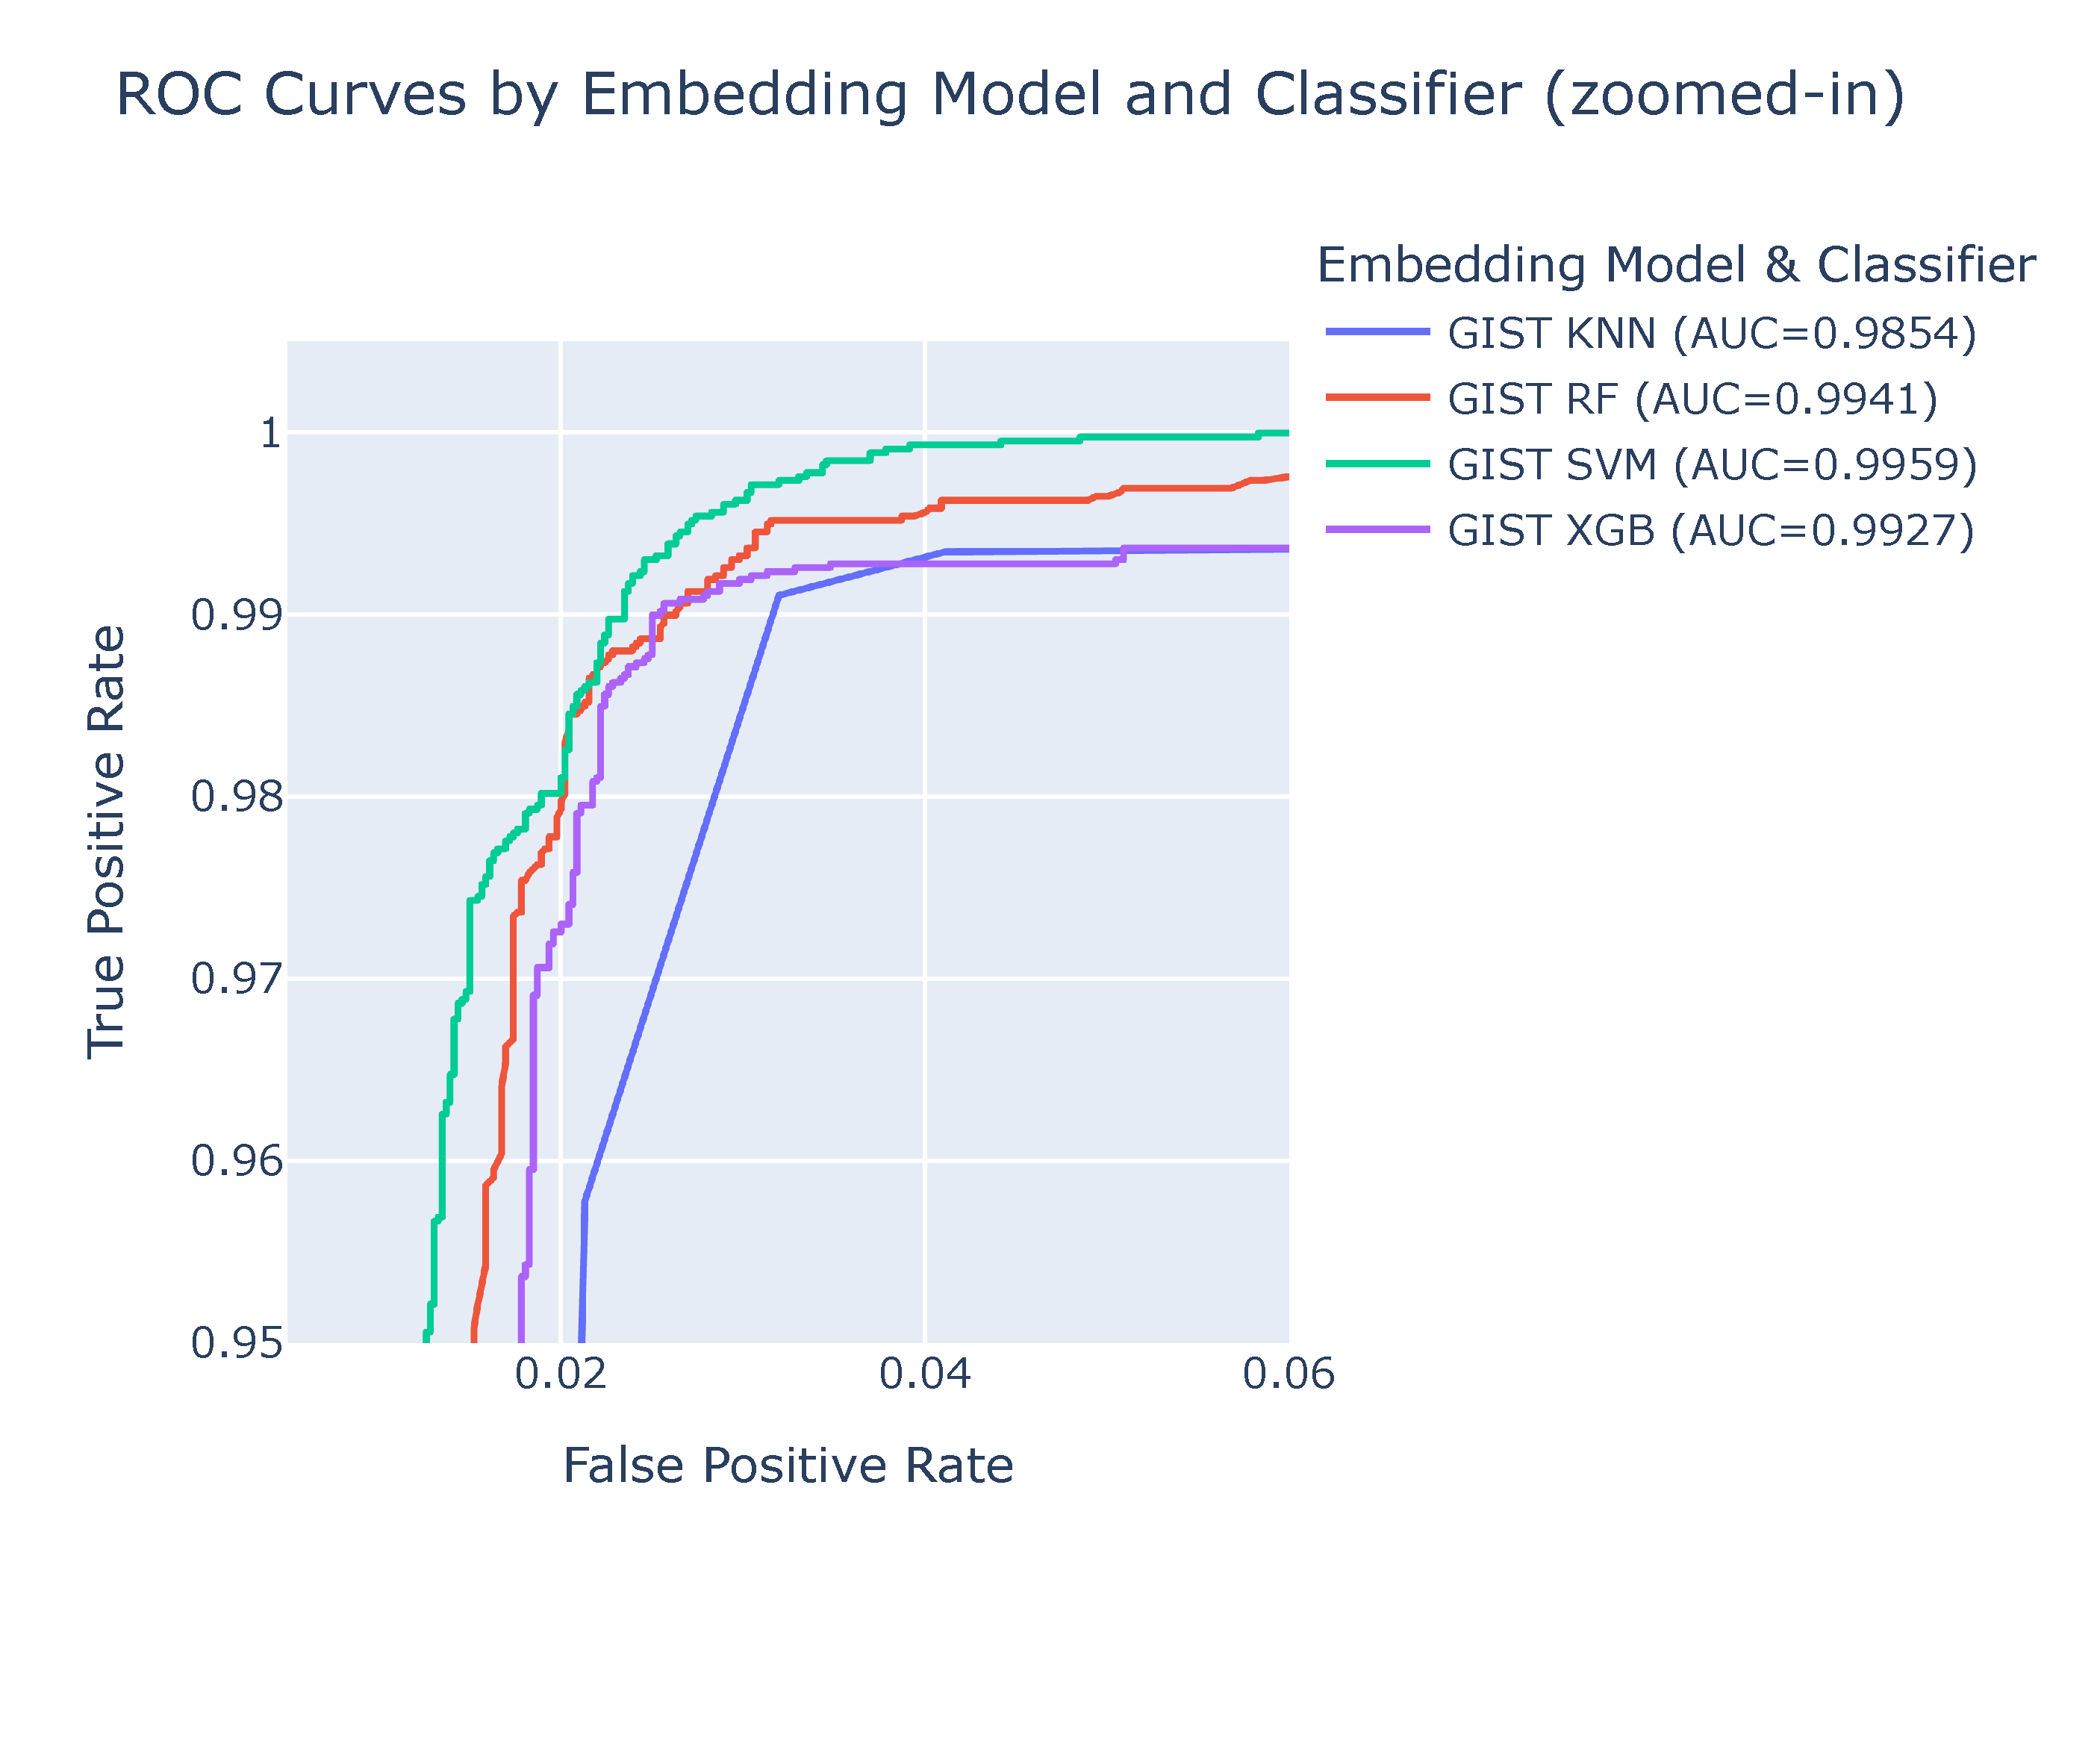
\includegraphics[width=0.37\textwidth,trim={18mm 50mm 180mm 50mm},clip]{roc_curves_gist_zoomed.pdf}\label{fig:gist_roc_zoomed}
    }
    \captionsetup[subfigure]{oneside,margin={-2.5cm,0cm}}
    \subfloat[Full Size]{
        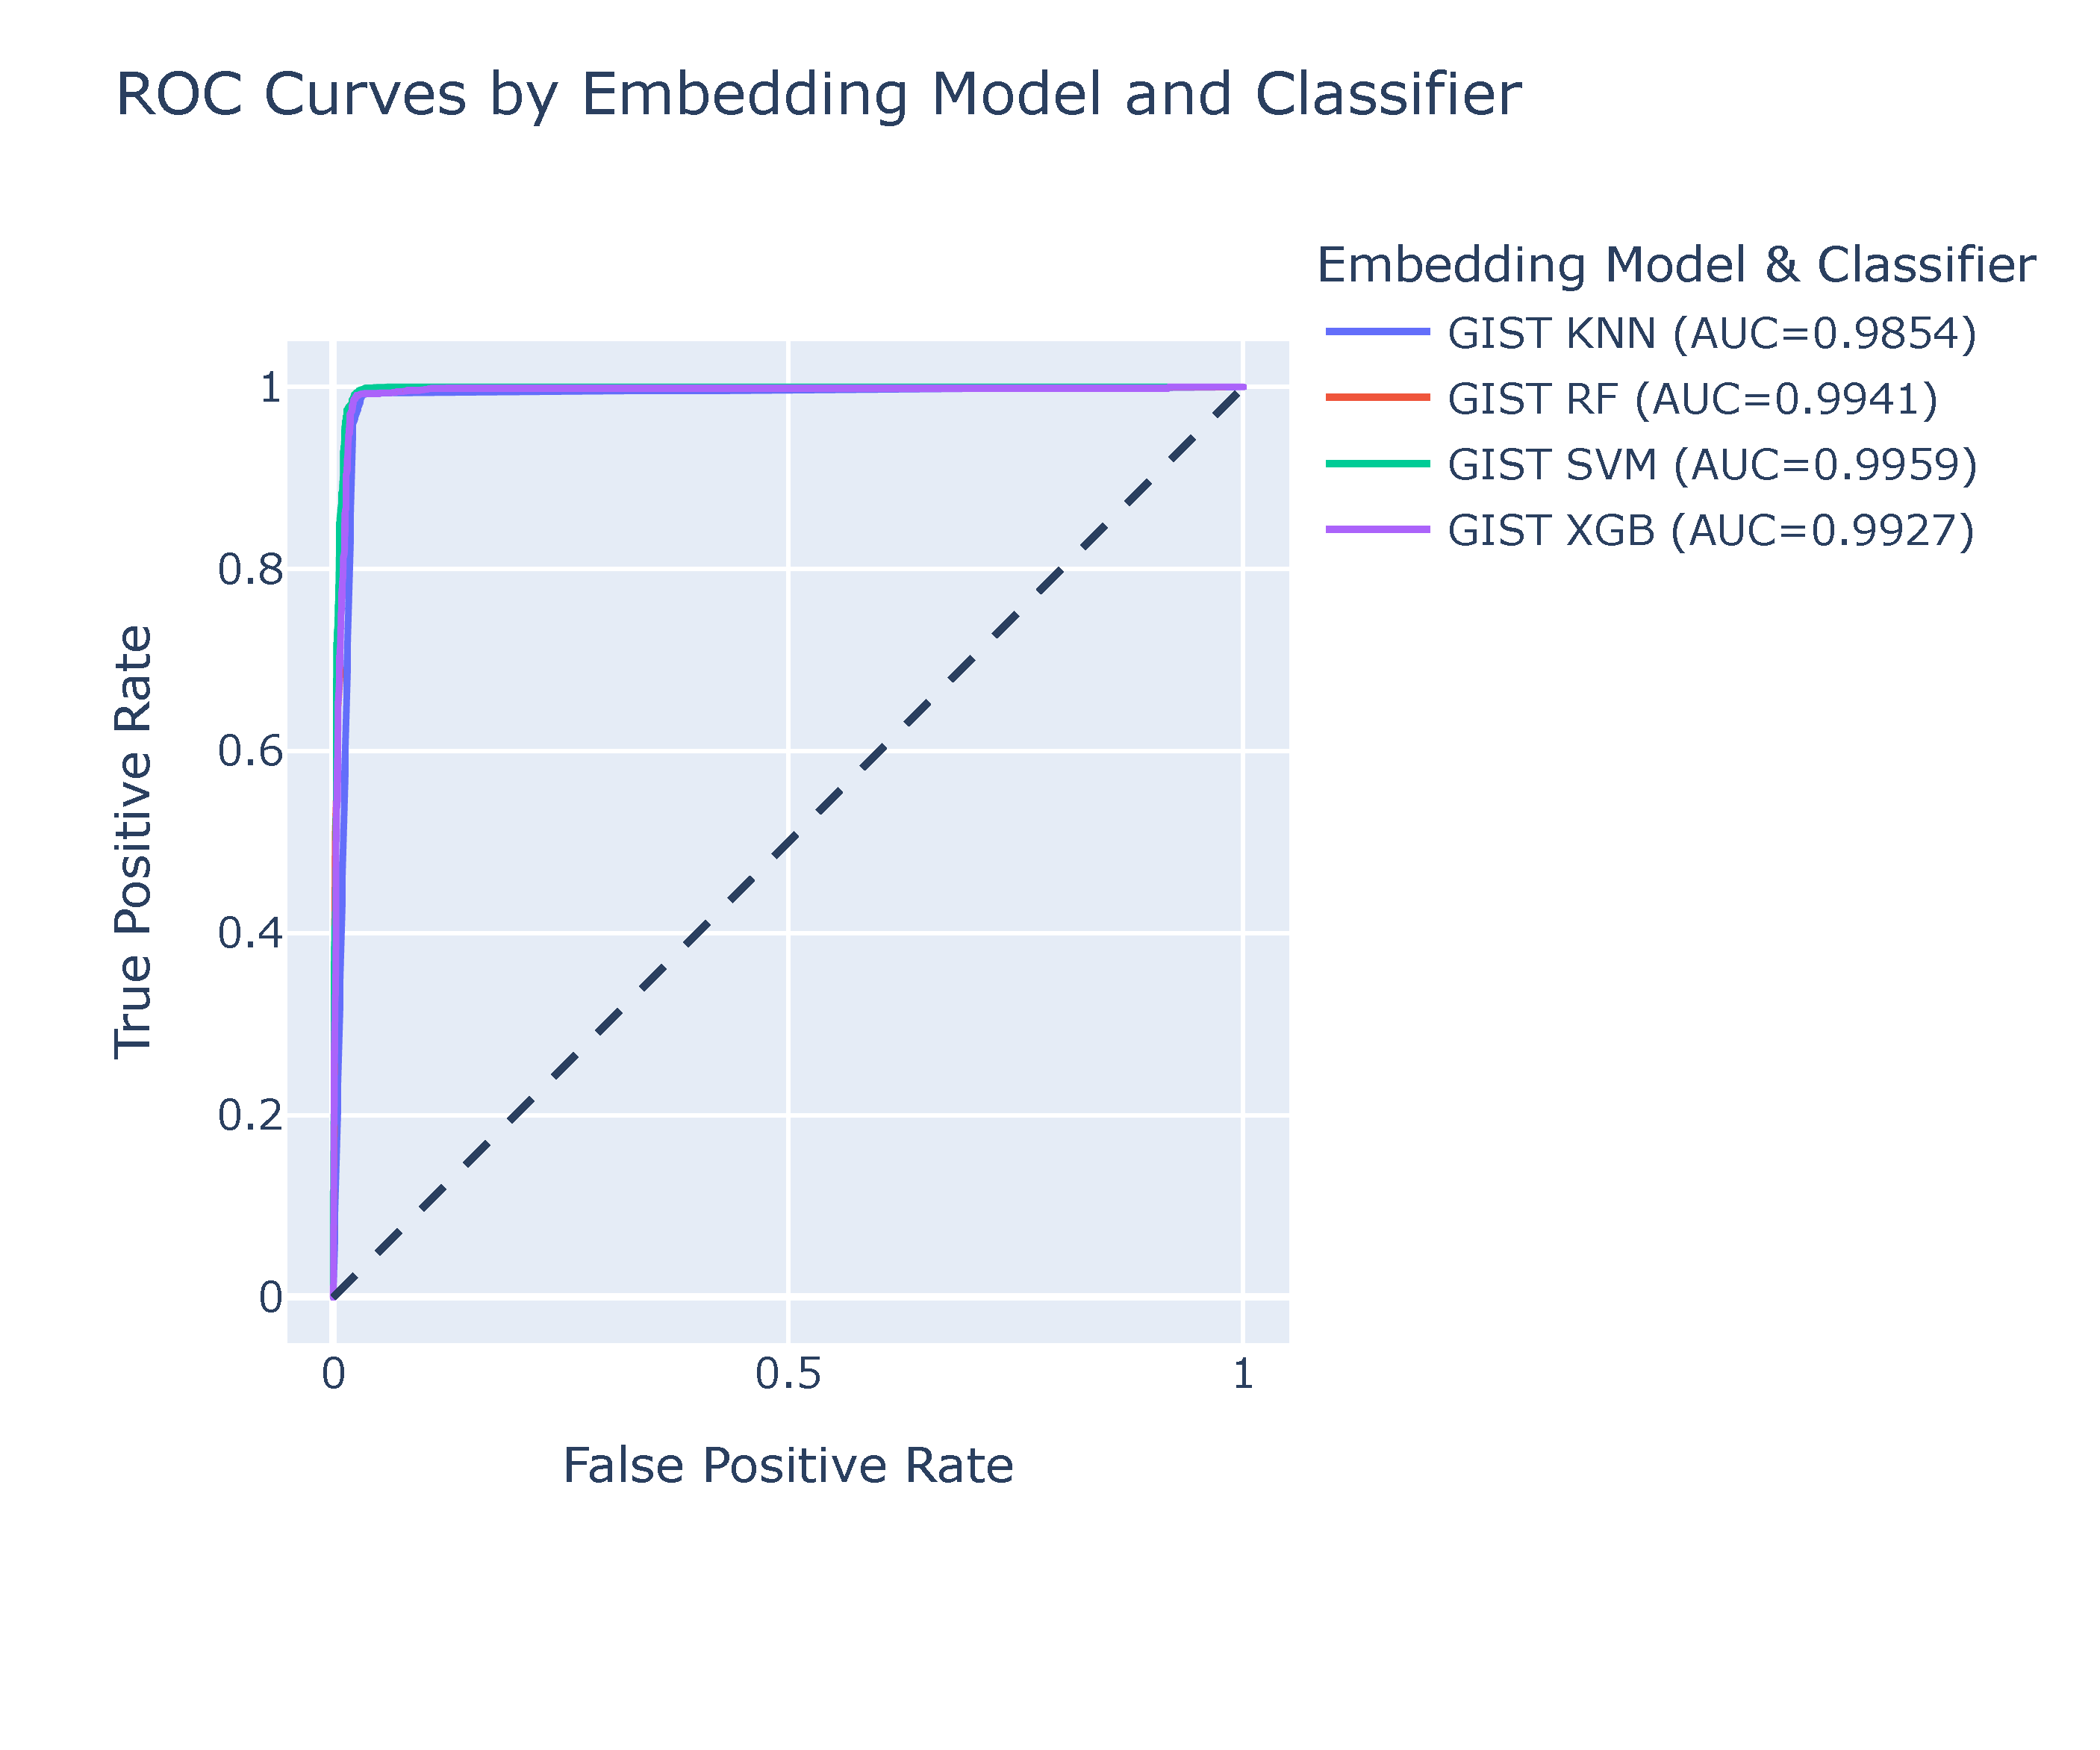
\includegraphics[width=0.58\textwidth,trim={25mm 50mm 12mm 50mm},clip]{roc_curves_gist.pdf}\label{fig:gist_roc_unzoomed}
    }
    \caption{GIST ROC Curves for Finalist Classifiers with Test Data}
\end{figure}

\begin{figure}[!h]
    \captionsetup{skip=5pt}
    \centering
    \captionsetup[subfigure]{oneside,margin={1cm,0cm}}
    \subfloat[Zoomed]{
        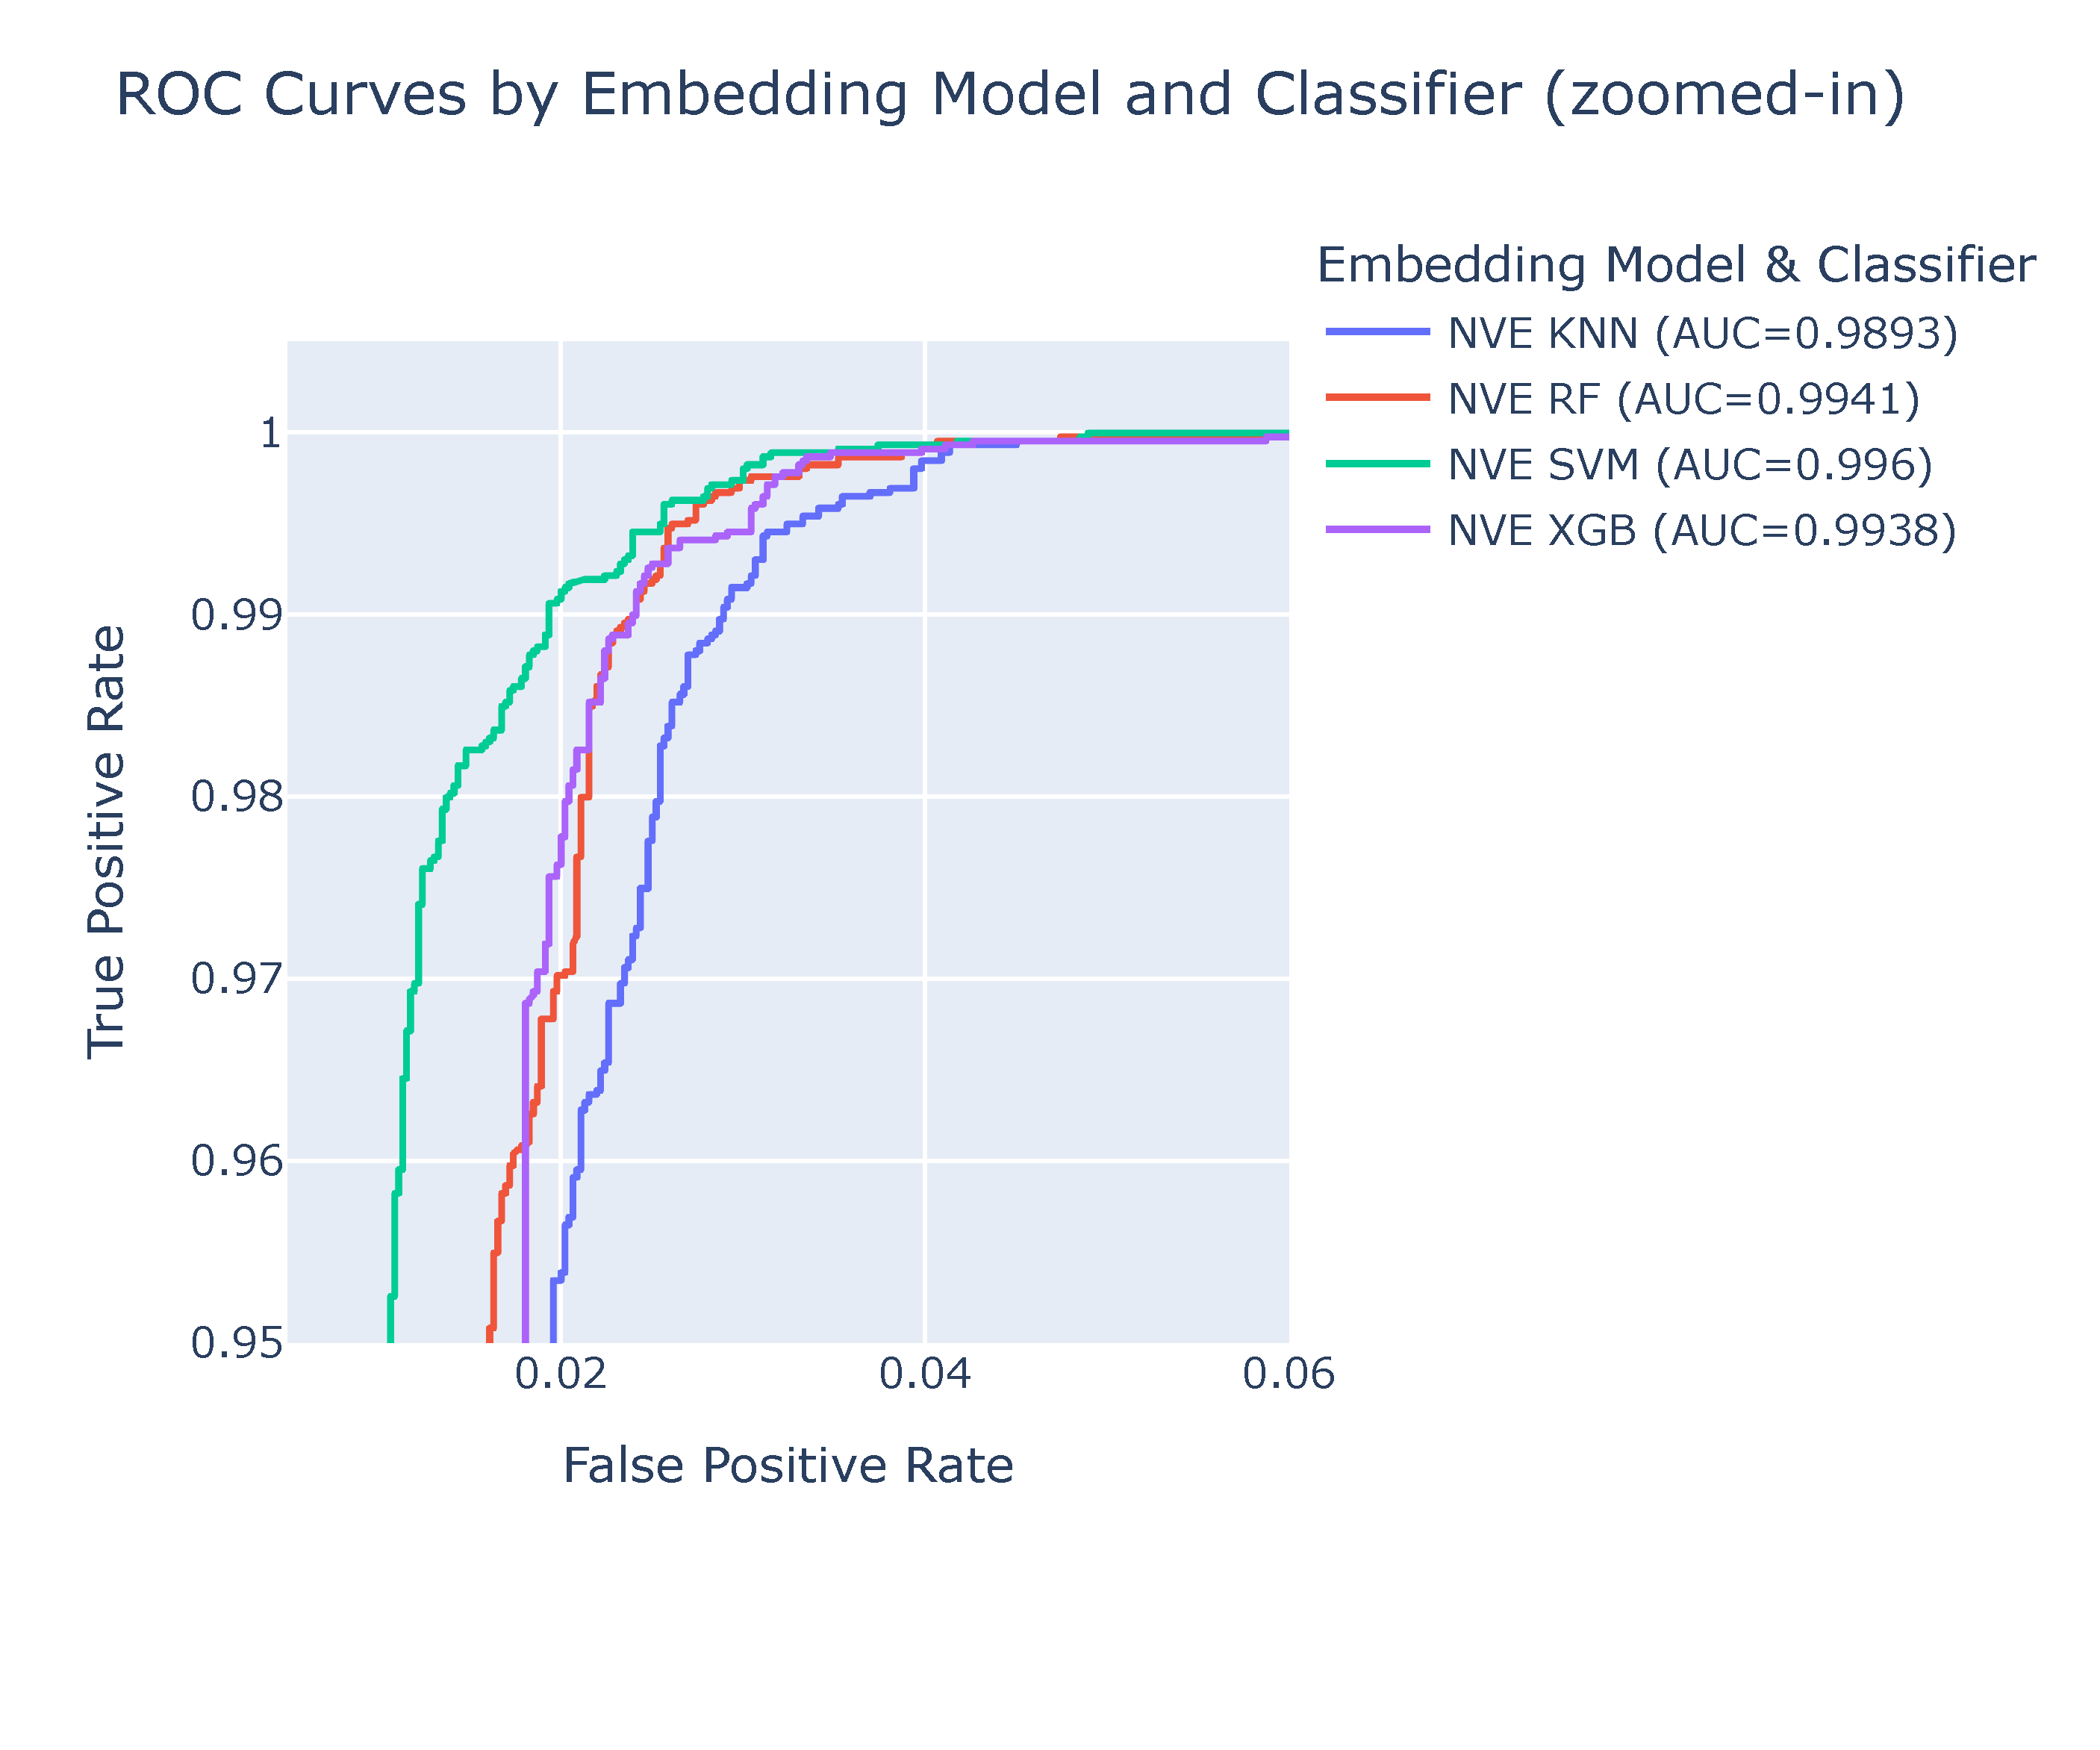
\includegraphics[width=0.37\textwidth,trim={18mm 50mm 180mm 50mm},clip]{roc_curves_nve_zoomed.pdf}\label{fig:nve_roc_zoomed}
    }
    \captionsetup[subfigure]{oneside,margin={-2.5cm,0cm}}
    \subfloat[Full Size]{
        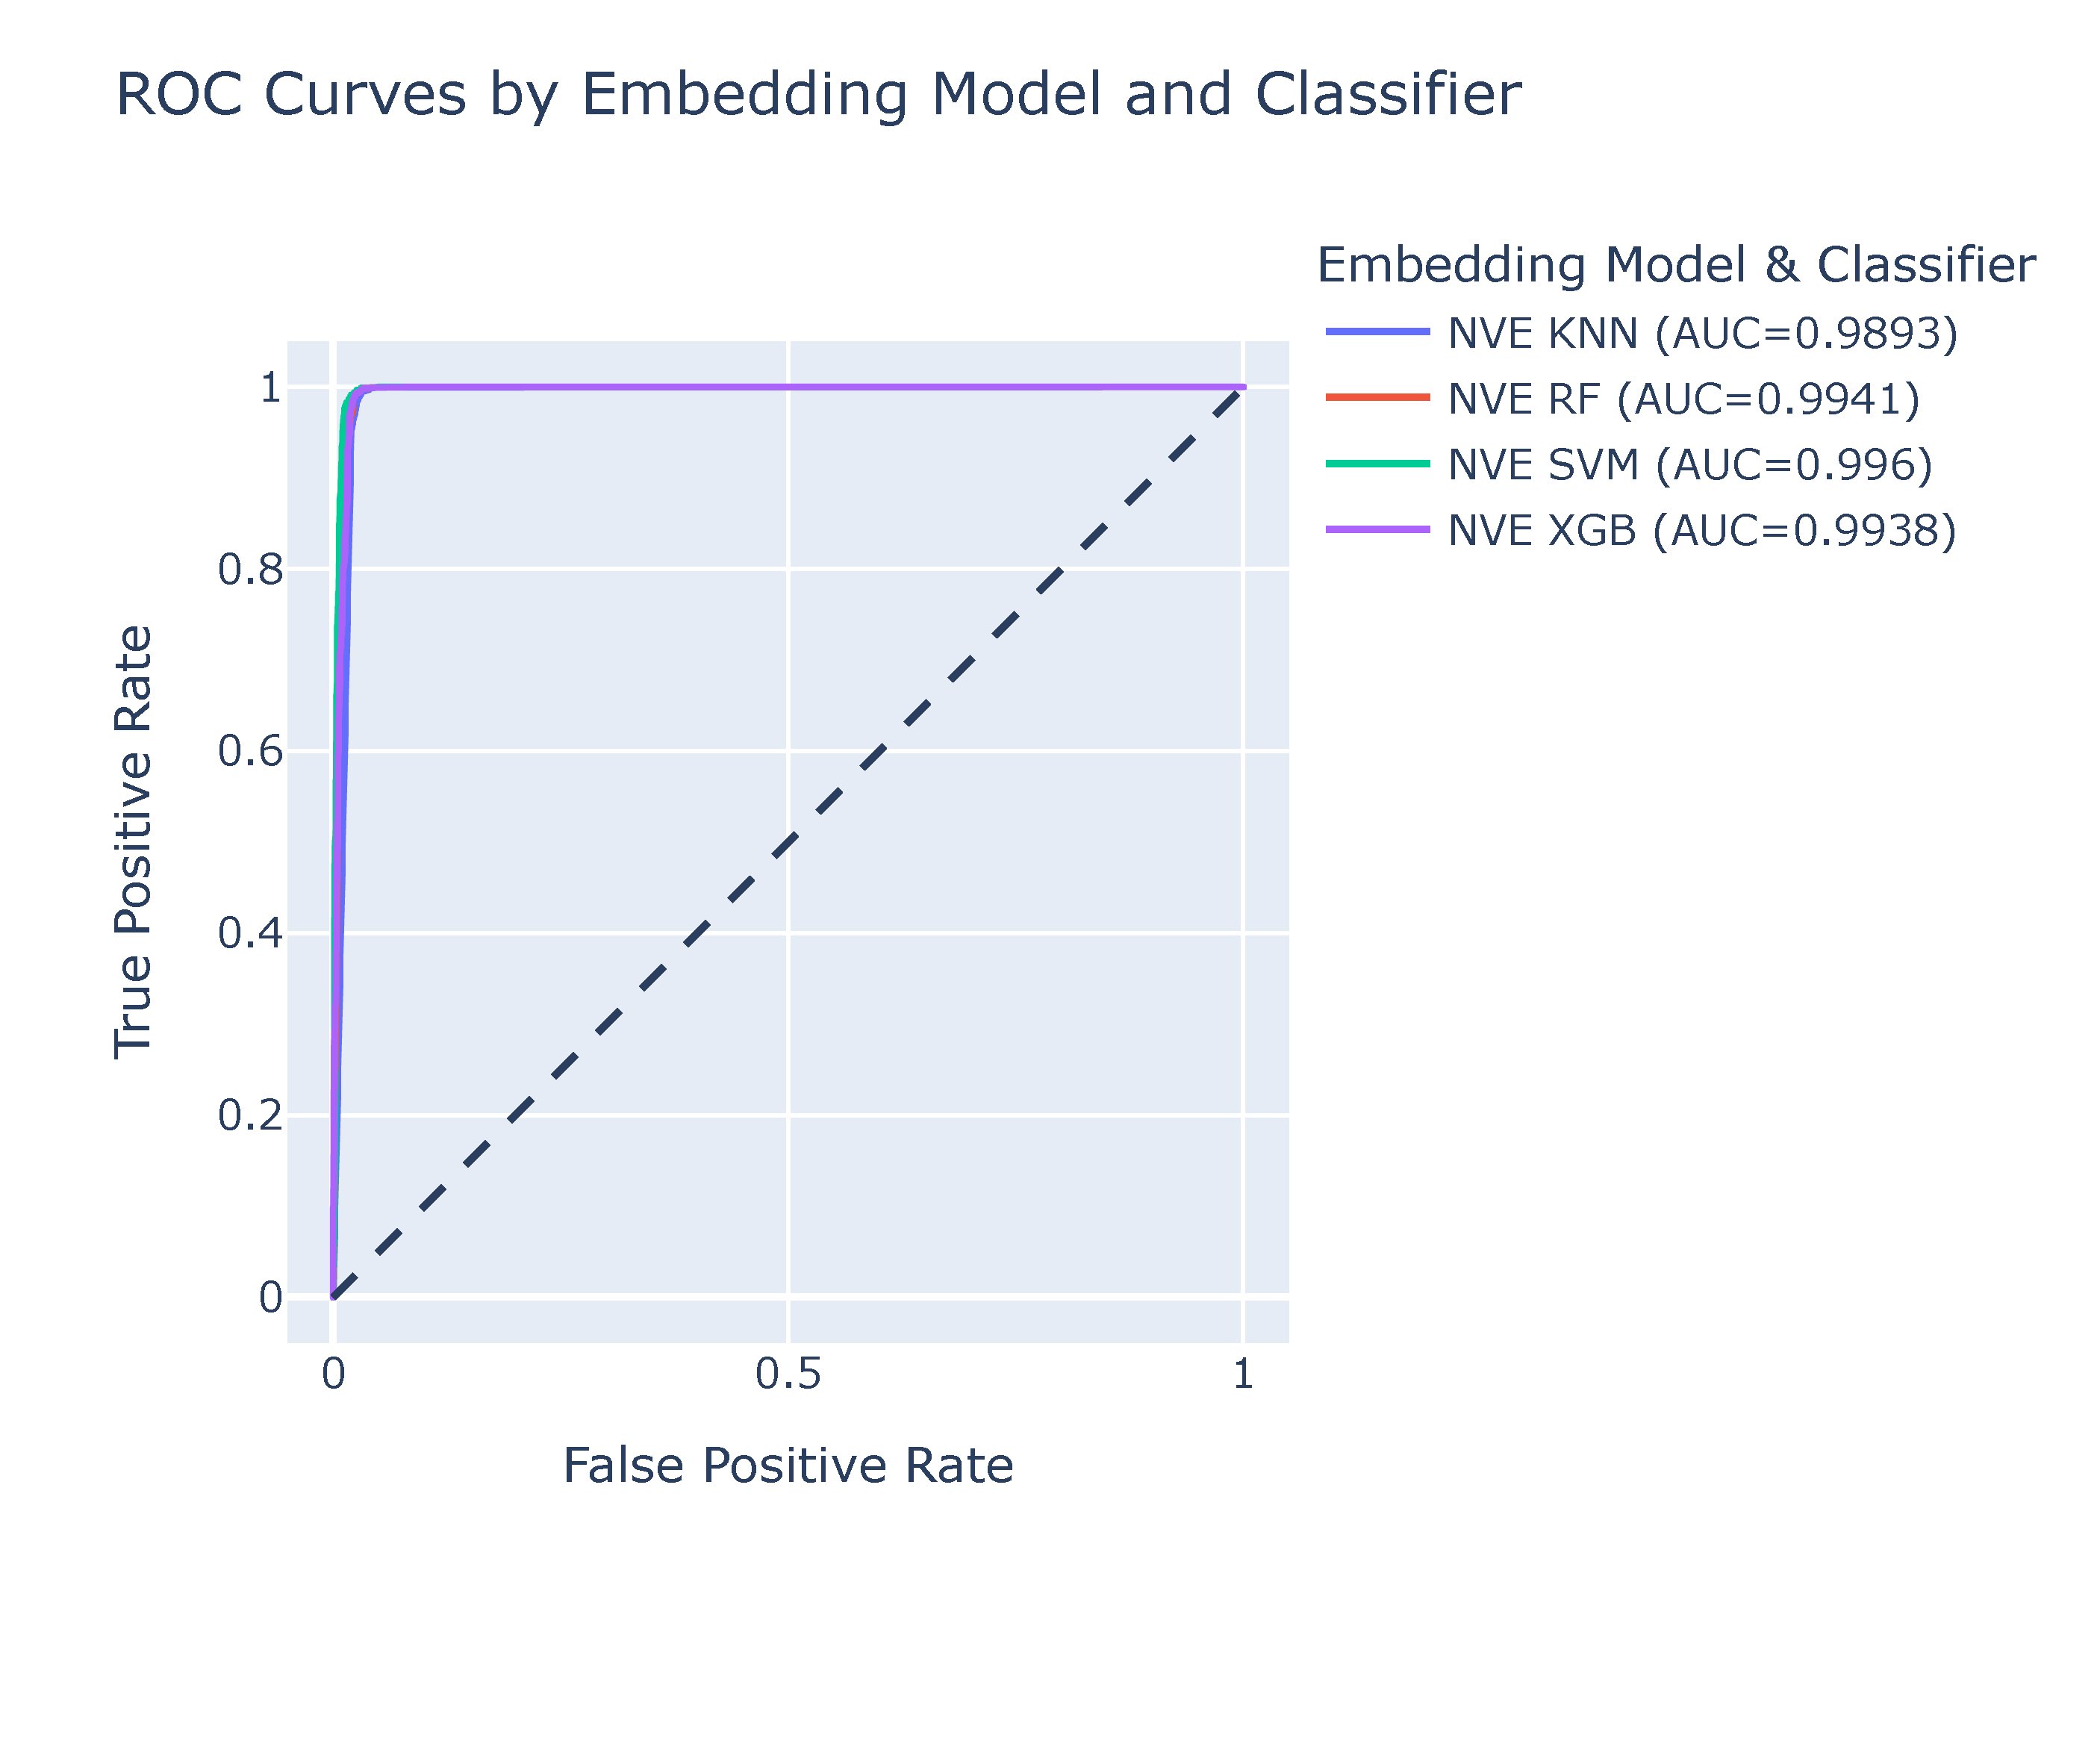
\includegraphics[width=0.58\textwidth,trim={25mm 50mm 12mm 50mm},clip]{roc_curves_nve.pdf}\label{fig:nve_roc_unzoomed}
    }
    \caption{NVE ROC Curves for Finalist Classifiers with Test Data}
\end{figure}

\begin{figure}[h!]
    \captionsetup{skip=5pt}
    \centering
    \captionsetup[subfigure]{oneside,margin={1cm,0cm}}
    \subfloat[Zoomed]{
        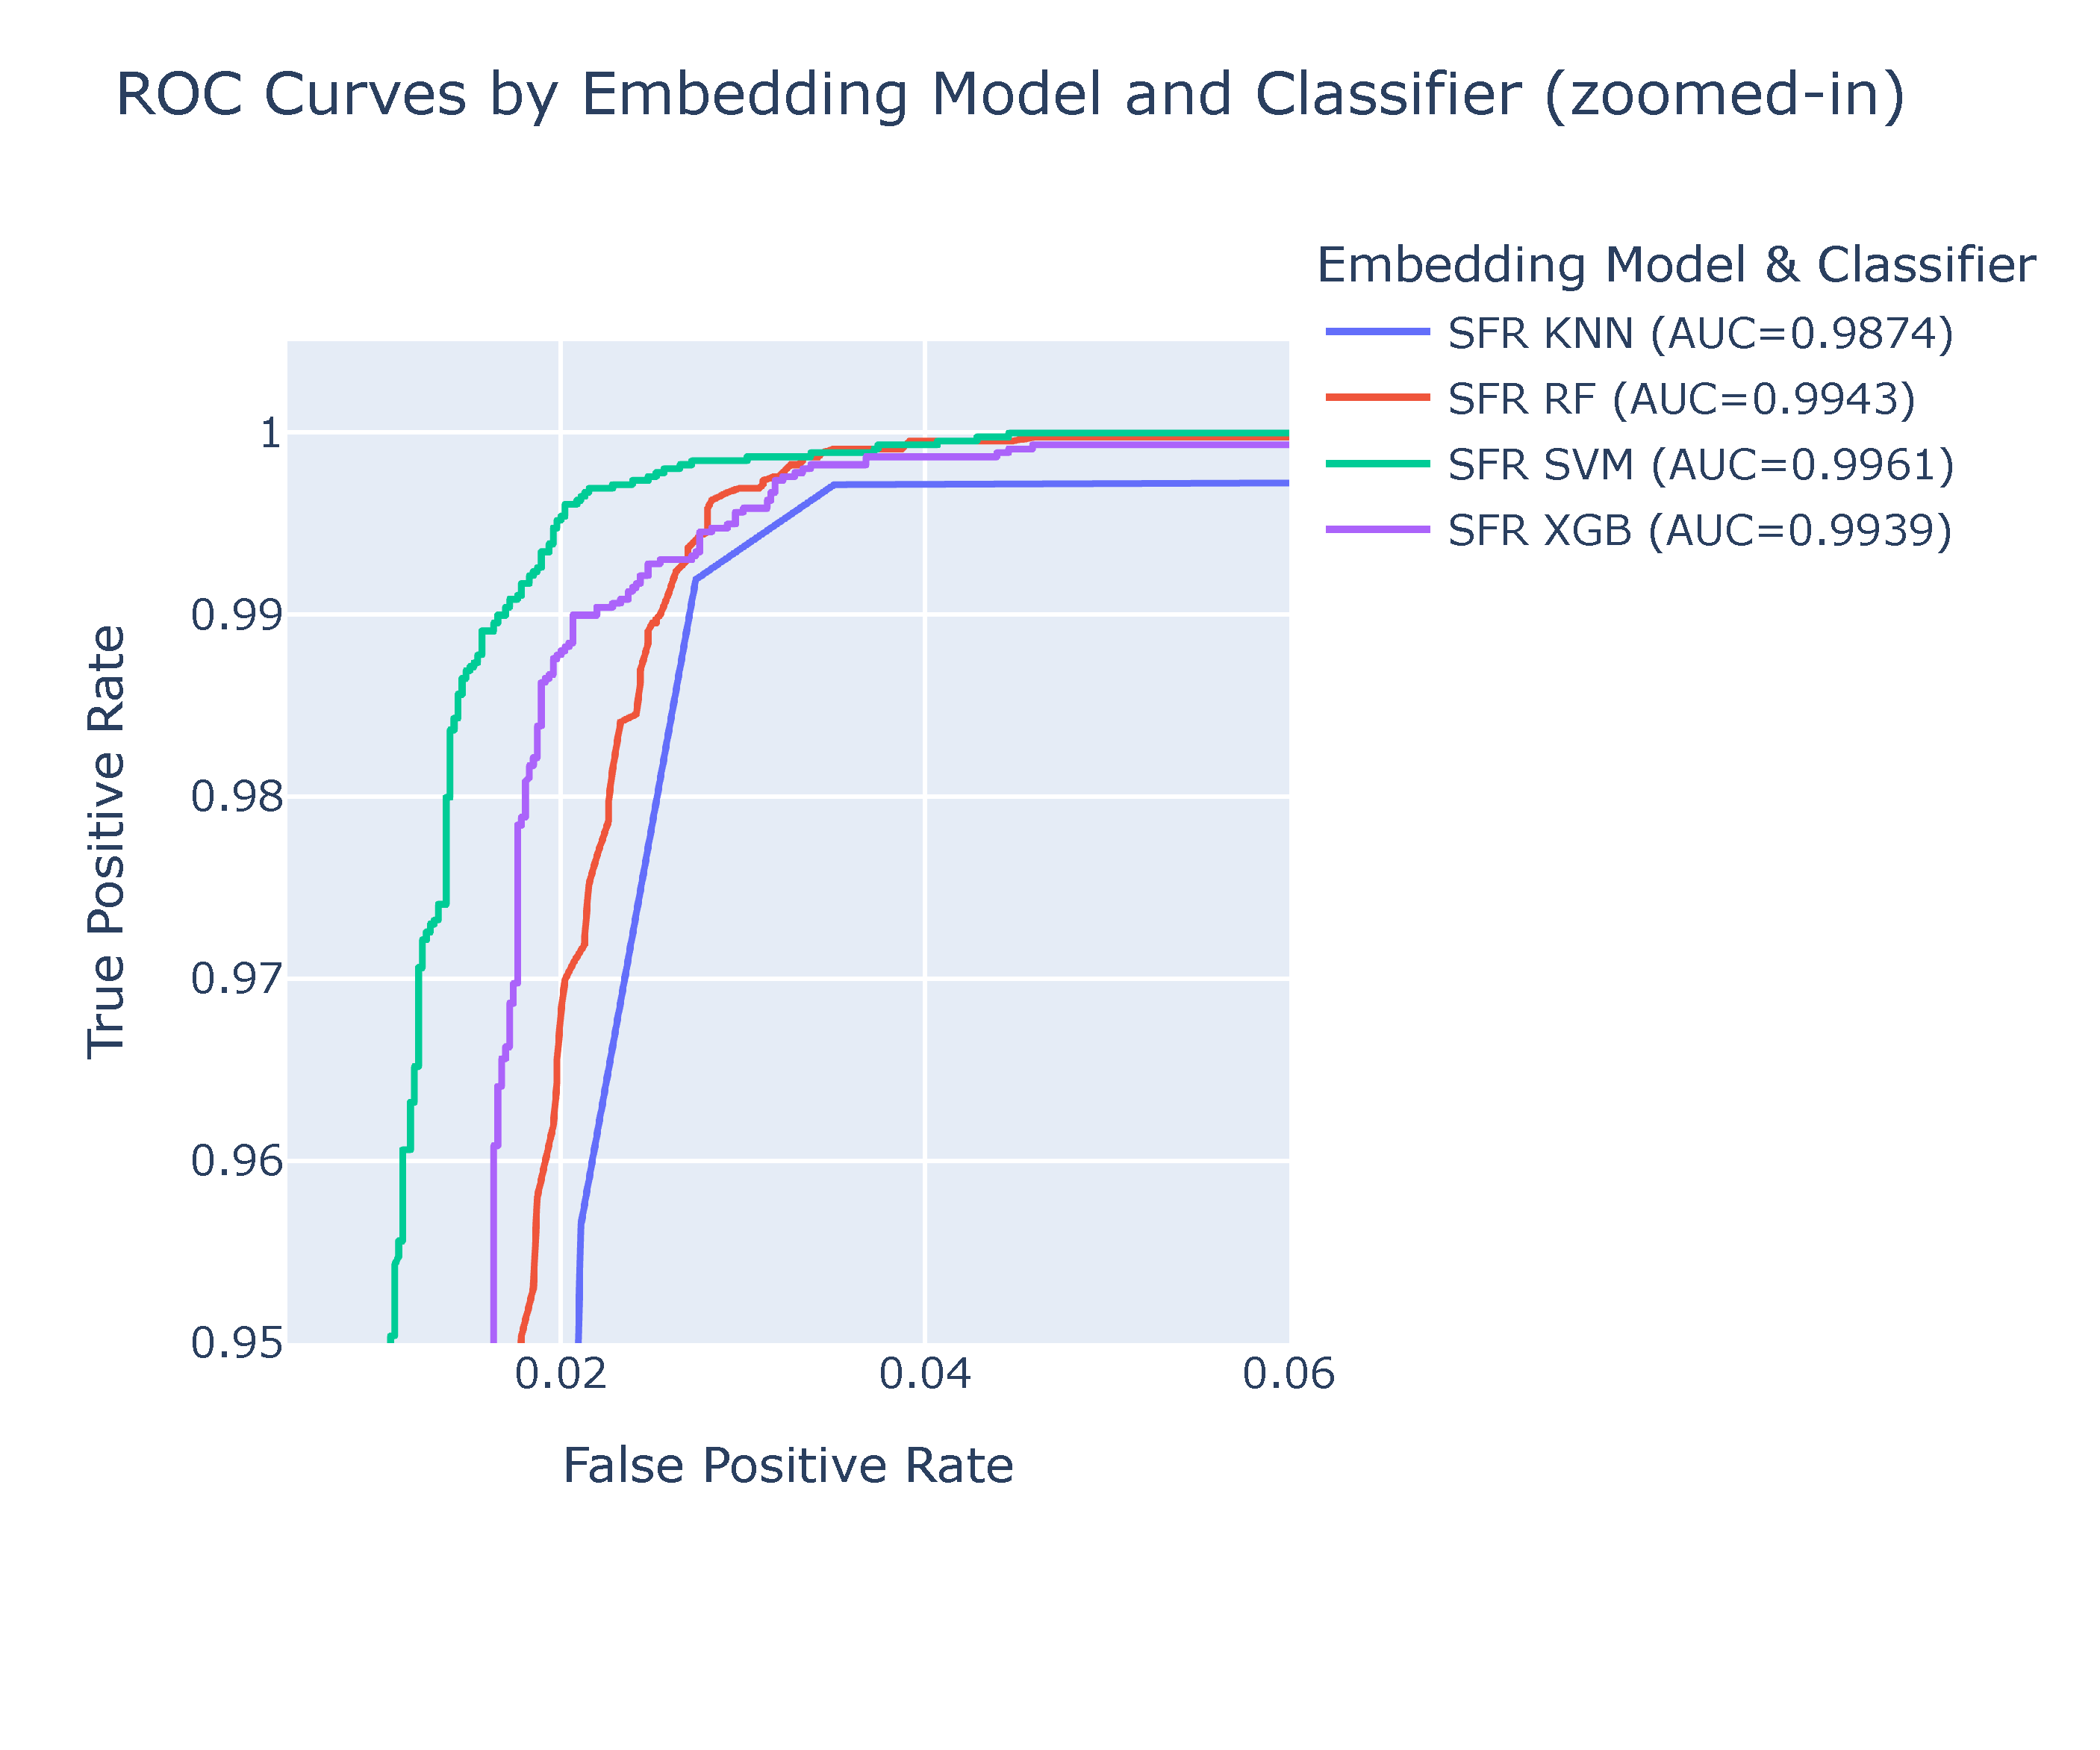
\includegraphics[width=0.37\textwidth,trim={18mm 50mm 180mm 50mm},clip]{roc_curves_sfr_zoomed.pdf}\label{fig:sfr_roc_zoomed}
    }
    \captionsetup[subfigure]{oneside,margin={-2.5cm,0cm}}
    \subfloat[Full Size]{
        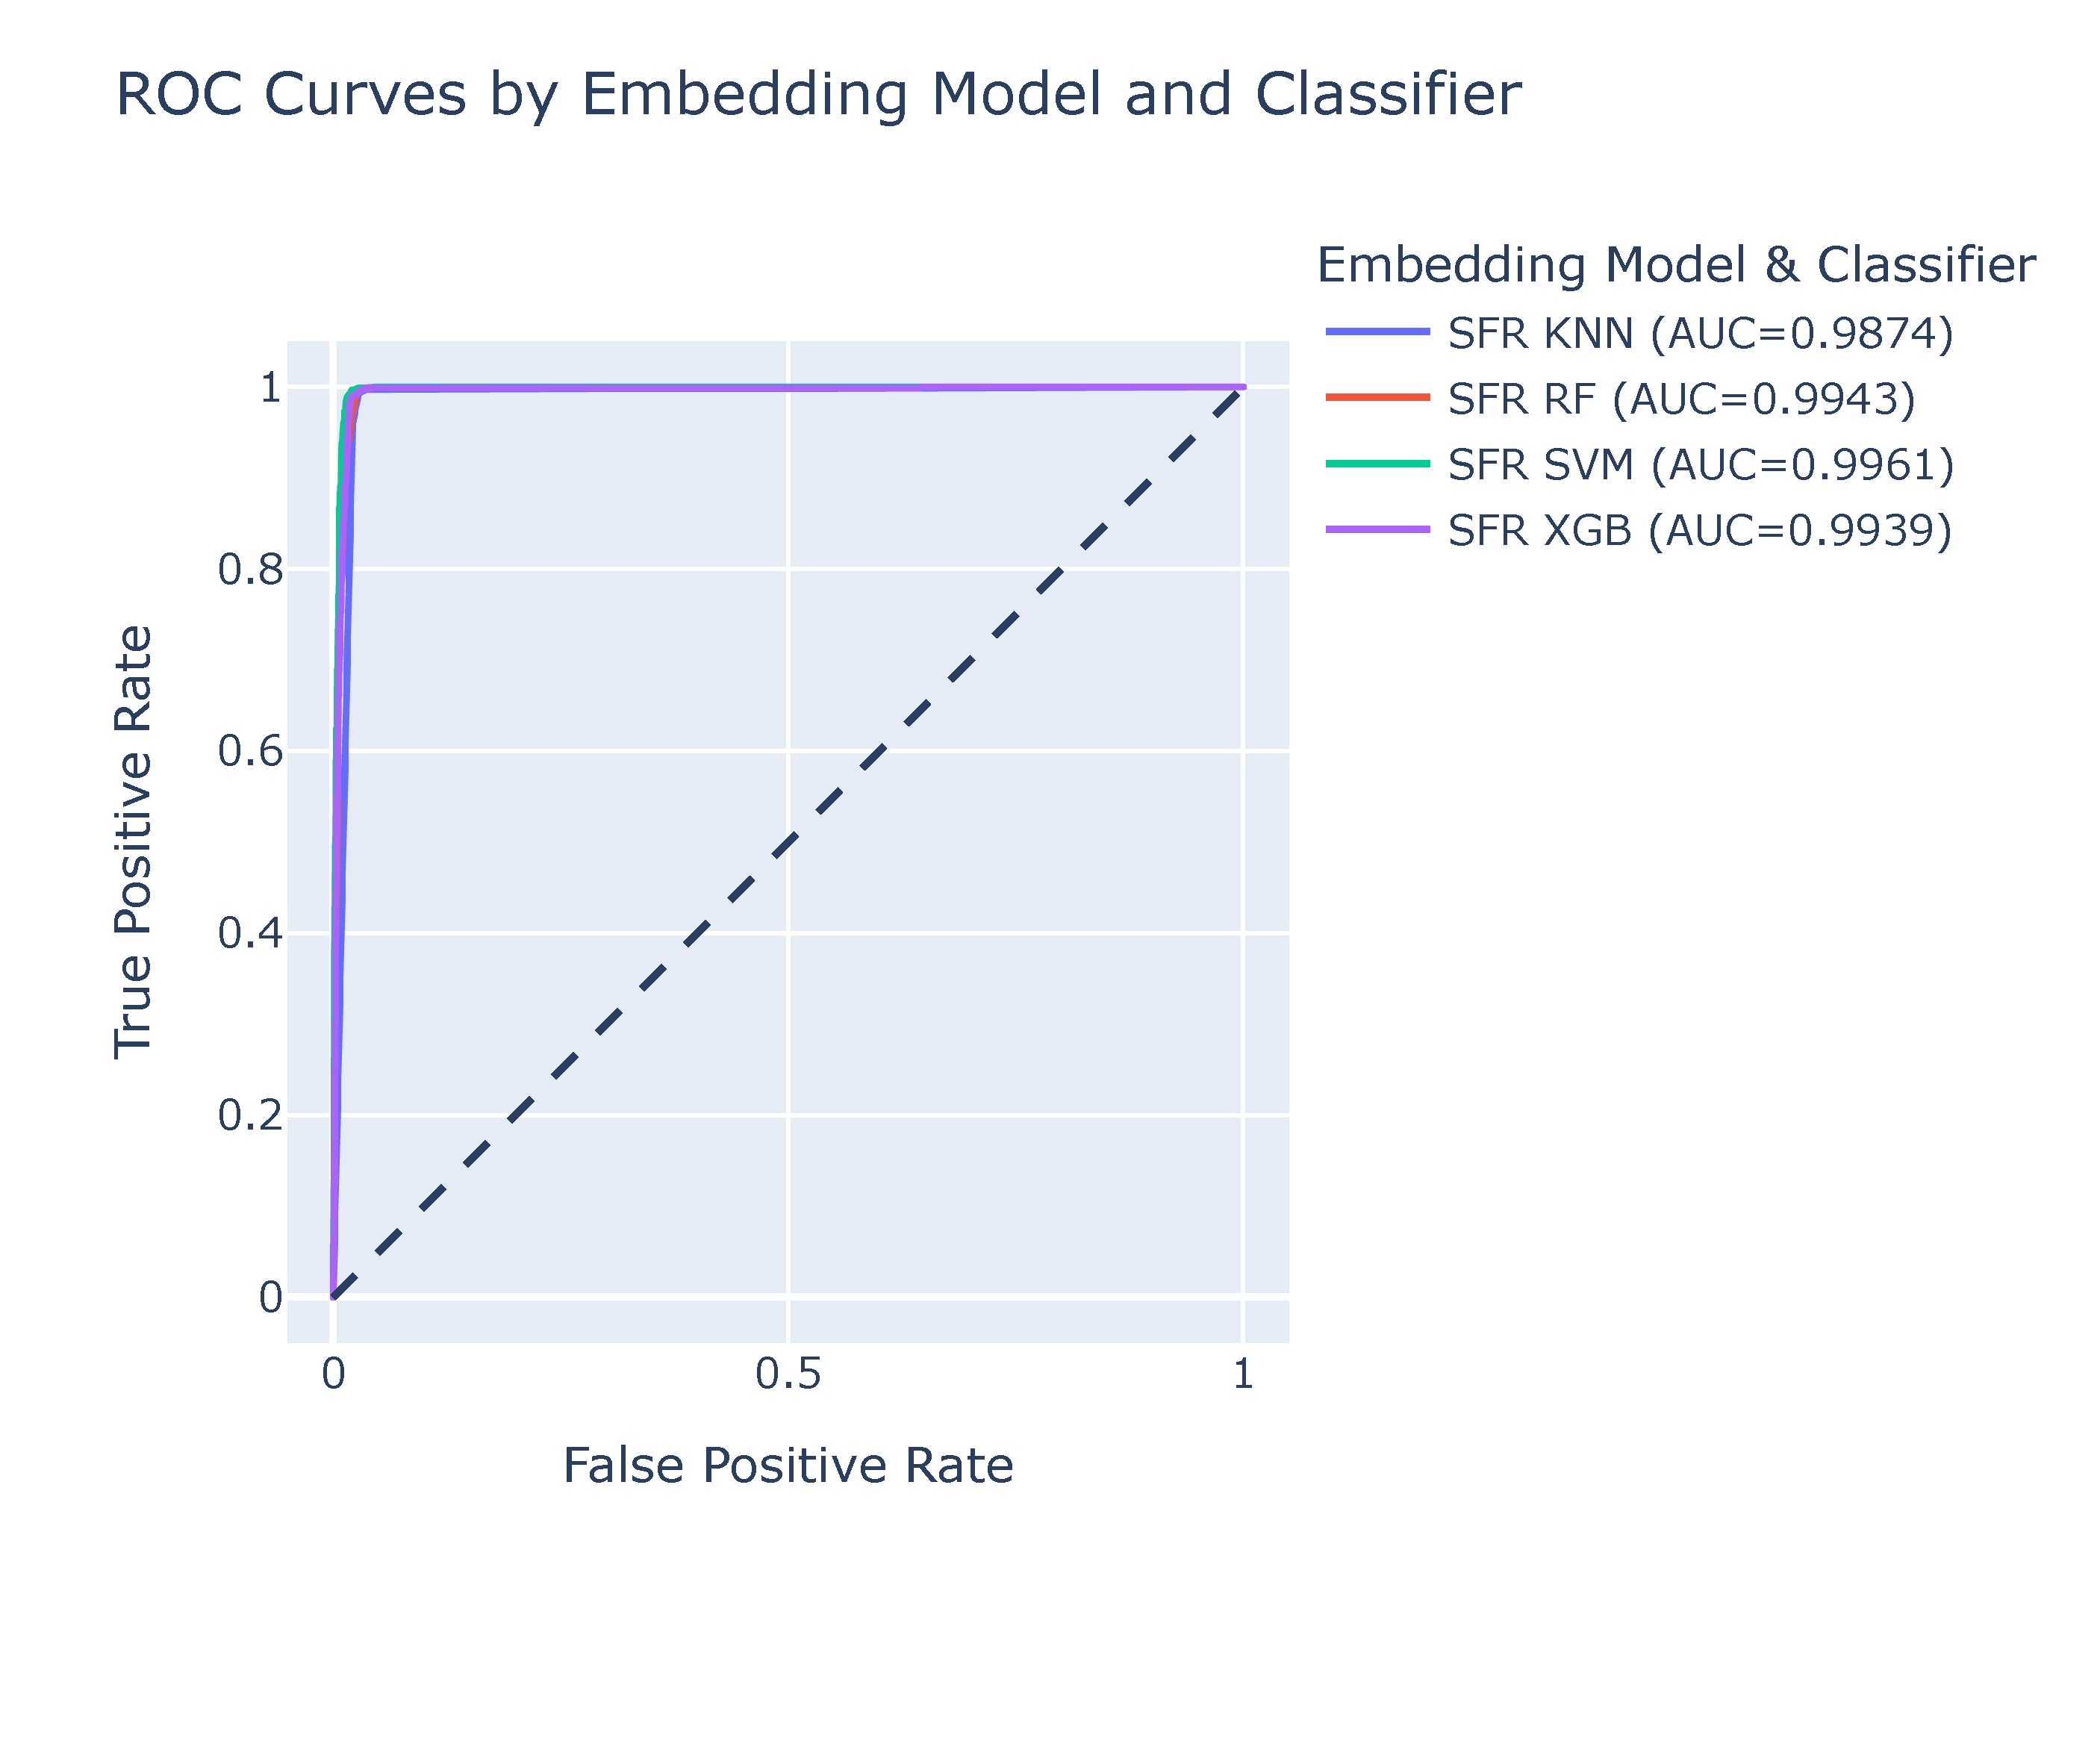
\includegraphics[width=0.58\textwidth,trim={25mm 50mm 12mm 50mm},clip]{roc_curves_sfr.pdf}\label{fig:sfr_roc_unzoomed}
    }
    \caption{SFR ROC Curves for Finalist Classifiers with Test Data}
\end{figure}

\clearpage
\section{Confusion Matrices}

\begin{figure}[!h]
    \captionsetup{skip=5pt}
    \centering
    \captionsetup[subfigure]{oneside,margin={1.3cm,0cm}}
    \subfloat[KNN]{
        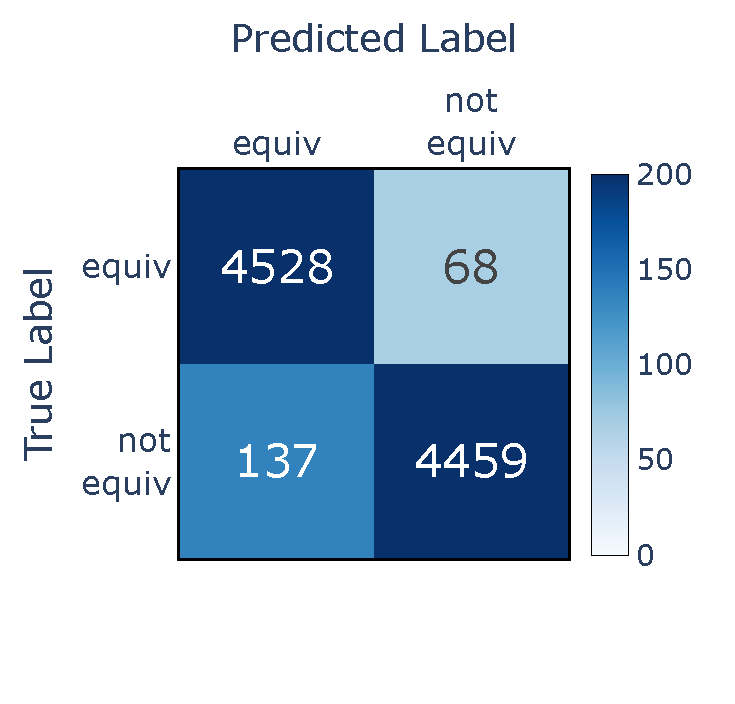
\includegraphics[width=0.277\textwidth,trim={0 23mm 26mm 0},clip]{cm_BGE_knn.pdf}
    }
    \captionsetup[subfigure]{oneside,margin={0cm,0cm}}
    \subfloat[Random Forest]{
        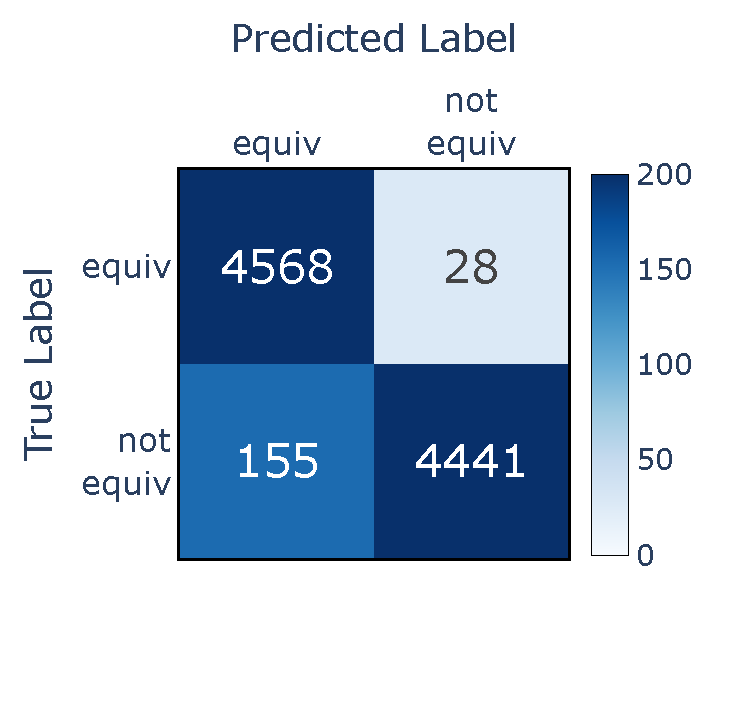
\includegraphics[width=0.194\textwidth,trim={29mm 23mm 26mm 0},clip]{cm_BGE_rf.pdf}
    }
    \captionsetup[subfigure]{oneside,margin={0cm,0cm}}
    \subfloat[SVM]{
        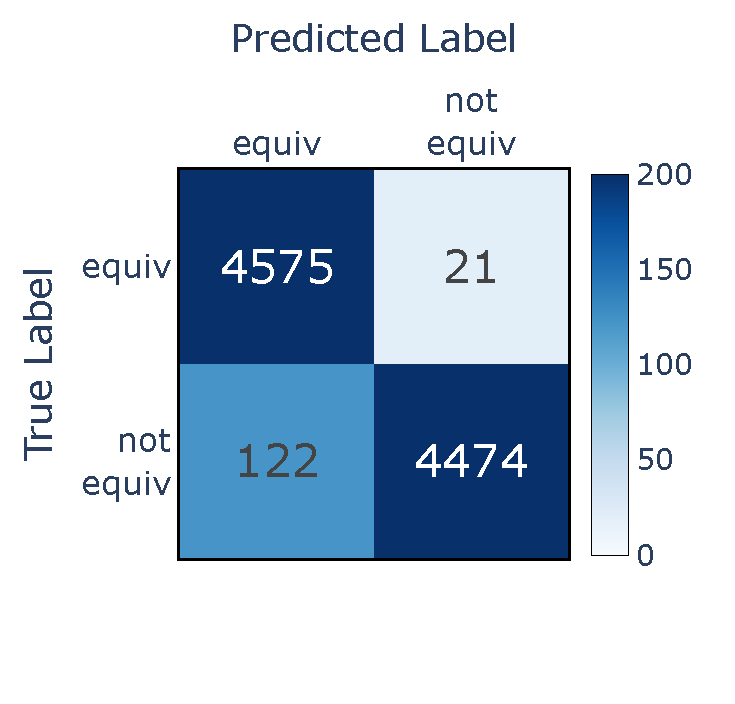
\includegraphics[width=0.194\textwidth,trim={29mm 23mm 26mm 0},clip]{cm_BGE_svm.pdf}
    }
    \captionsetup[subfigure]{oneside,margin={-1.25cm,0cm}}
    \subfloat[XGBoost]{
        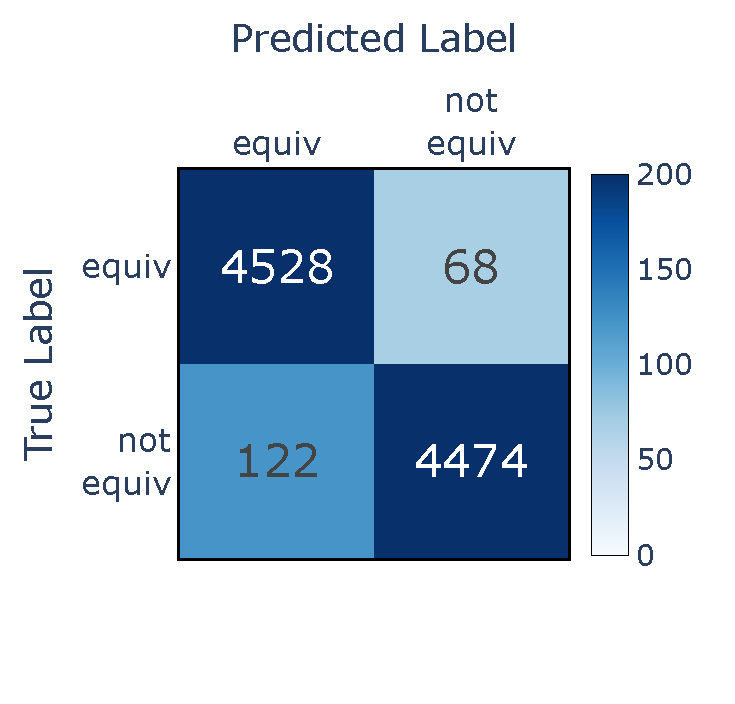
\includegraphics[width=0.246\textwidth,trim={29mm 23mm 7mm 0},clip]{cm_BGE_xgb.pdf}
    }
    \caption{BGE Confusion Matrices for Finalist Classifiers with Test Data}
\end{figure}

\begin{figure}[!h]
    \captionsetup{skip=5pt}
    \centering
    \captionsetup[subfigure]{oneside,margin={1.3cm,0cm}}
    \subfloat[KNN]{
        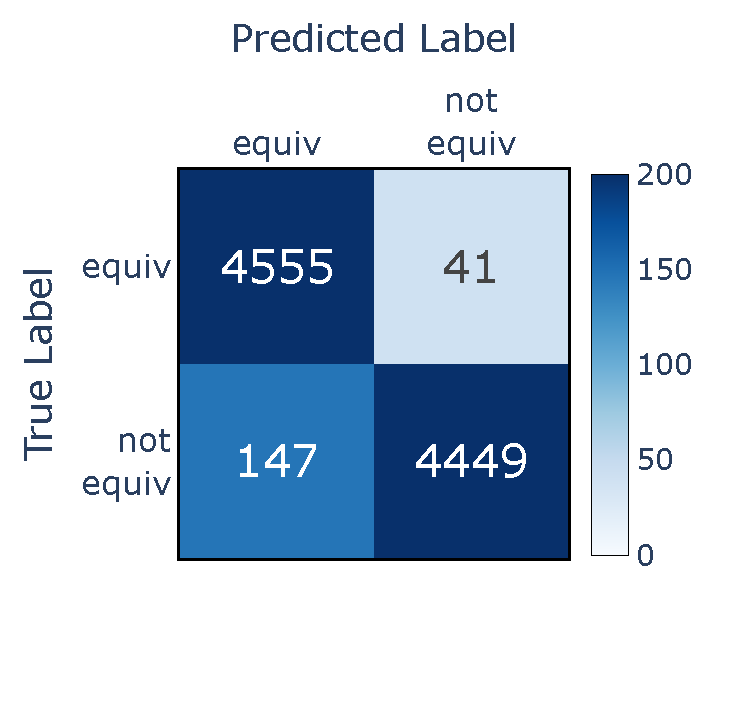
\includegraphics[width=0.277\textwidth,trim={0 23mm 26mm 0},clip]{cm_GIST_knn.pdf}
    }
    \captionsetup[subfigure]{oneside,margin={0cm,0cm}}
    \subfloat[Random Forest]{
        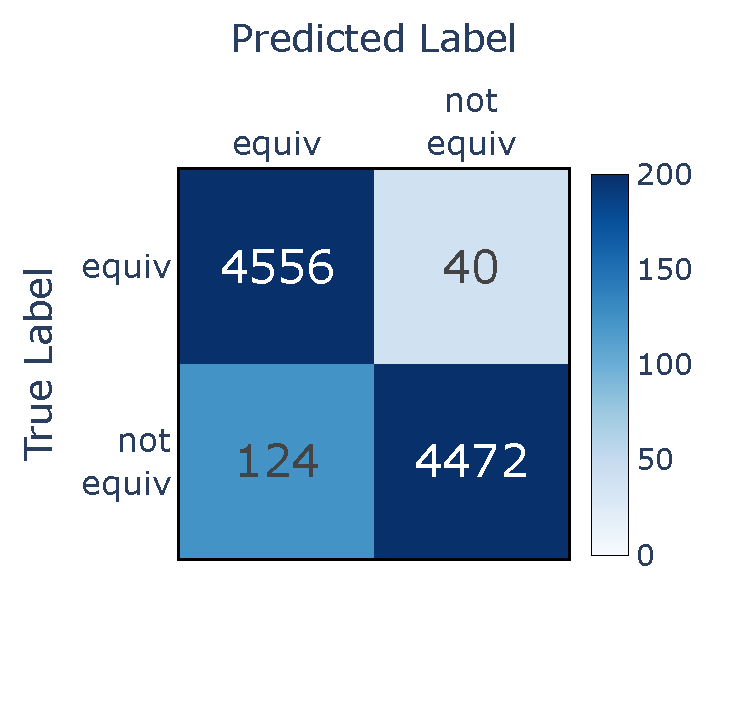
\includegraphics[width=0.194\textwidth,trim={29mm 23mm 26mm 0},clip]{cm_GIST_rf.pdf}
    }
    \captionsetup[subfigure]{oneside,margin={0cm,0cm}}
    \subfloat[SVM]{
        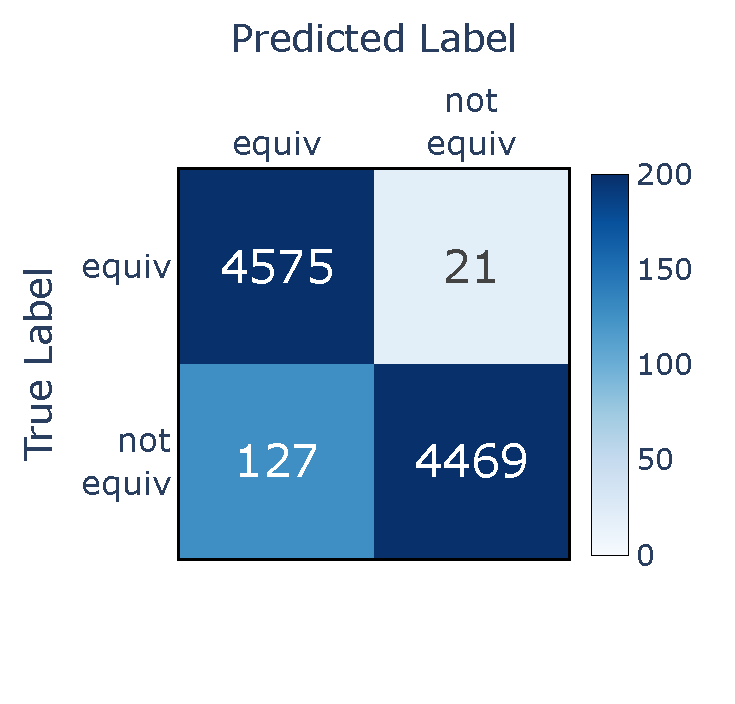
\includegraphics[width=0.194\textwidth,trim={29mm 23mm 26mm 0},clip]{cm_GIST_svm.pdf}
    }
    \captionsetup[subfigure]{oneside,margin={-1.25cm,0cm}}
    \subfloat[XGBoost]{
        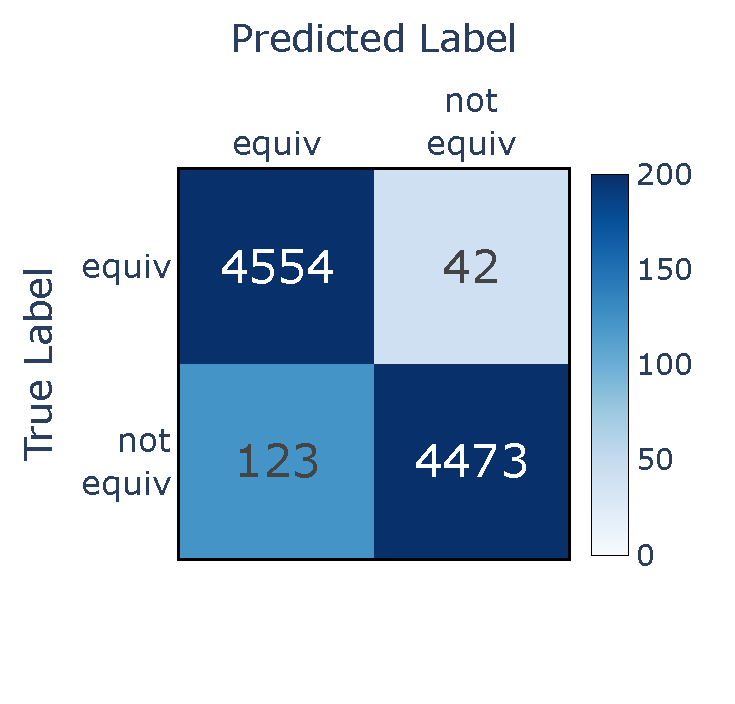
\includegraphics[width=0.246\textwidth,trim={29mm 23mm 7mm 0},clip]{cm_GIST_xgb.pdf}
    }
    \caption{GIST Confusion Matrices for Finalist Classifiers with Test Data}
\end{figure}

\begin{figure}[!h]
    \captionsetup{skip=5pt}
    \centering
    \captionsetup[subfigure]{oneside,margin={1.3cm,0cm}}
    \subfloat[KNN]{
        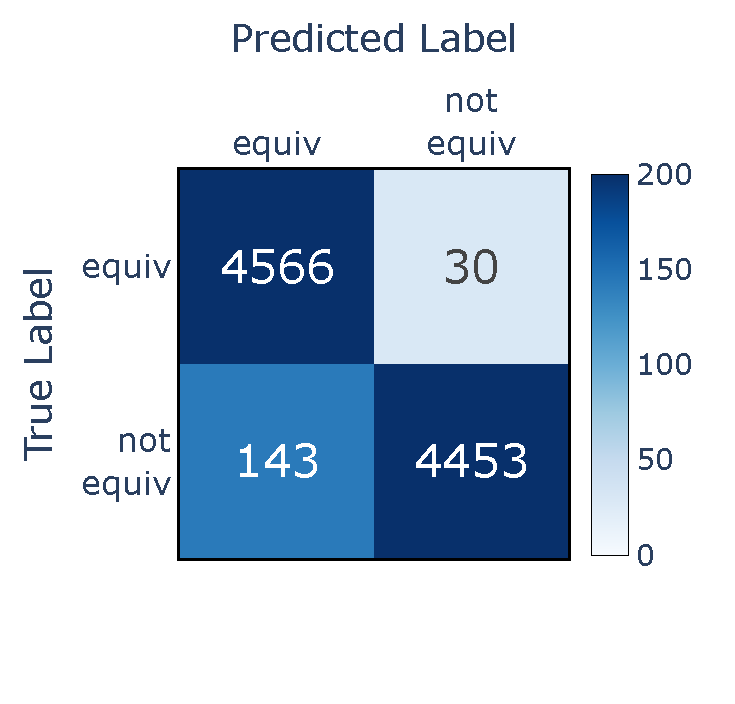
\includegraphics[width=0.277\textwidth,trim={0 23mm 26mm 0},clip]{cm_NVE_knn.pdf}
    }
    \captionsetup[subfigure]{oneside,margin={0cm,0cm}}
    \subfloat[Random Forest]{
        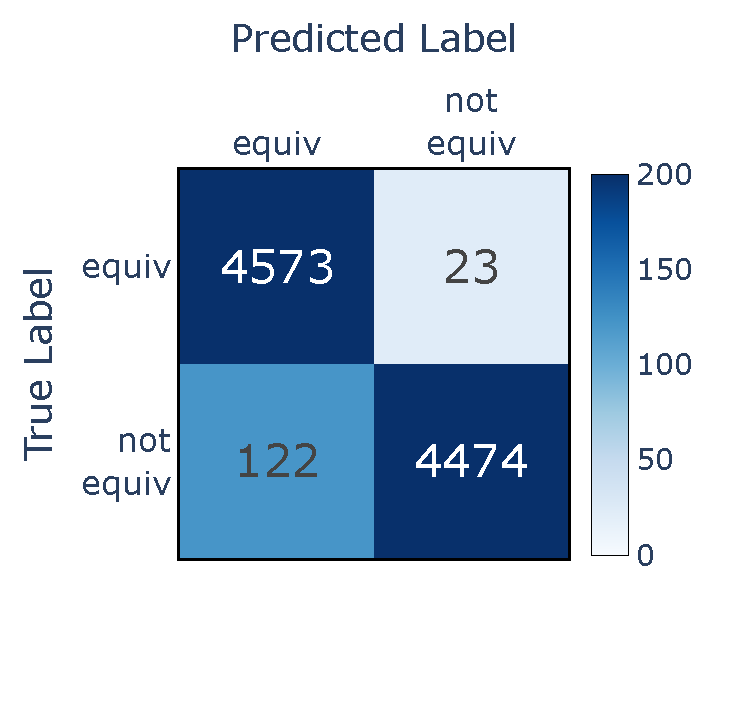
\includegraphics[width=0.194\textwidth,trim={29mm 23mm 26mm 0},clip]{cm_NVE_rf.pdf}
    }
    \captionsetup[subfigure]{oneside,margin={0cm,0cm}}
    \subfloat[SVM]{
        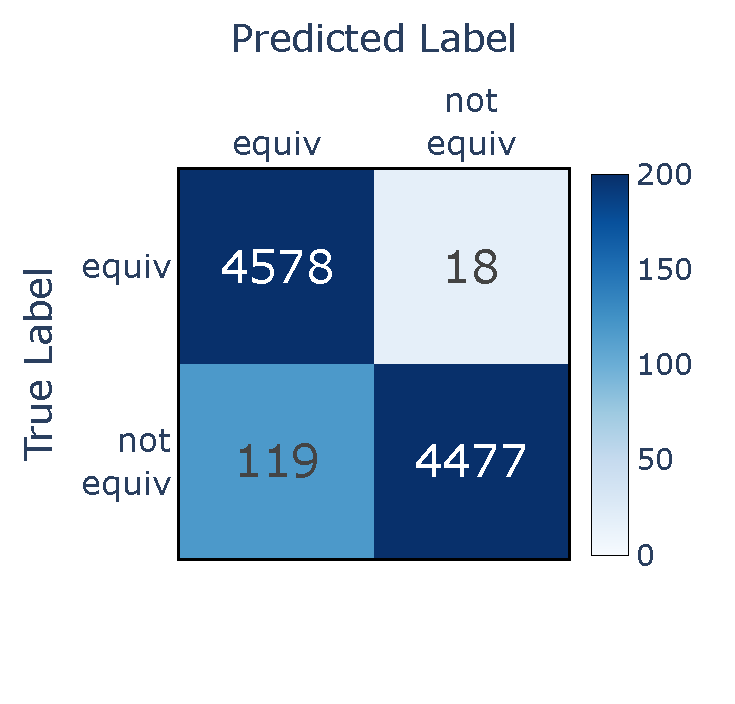
\includegraphics[width=0.194\textwidth,trim={29mm 23mm 26mm 0},clip]{cm_NVE_svm.pdf}
    }
    \captionsetup[subfigure]{oneside,margin={-1.25cm,0cm}}
    \subfloat[XGBoost]{
        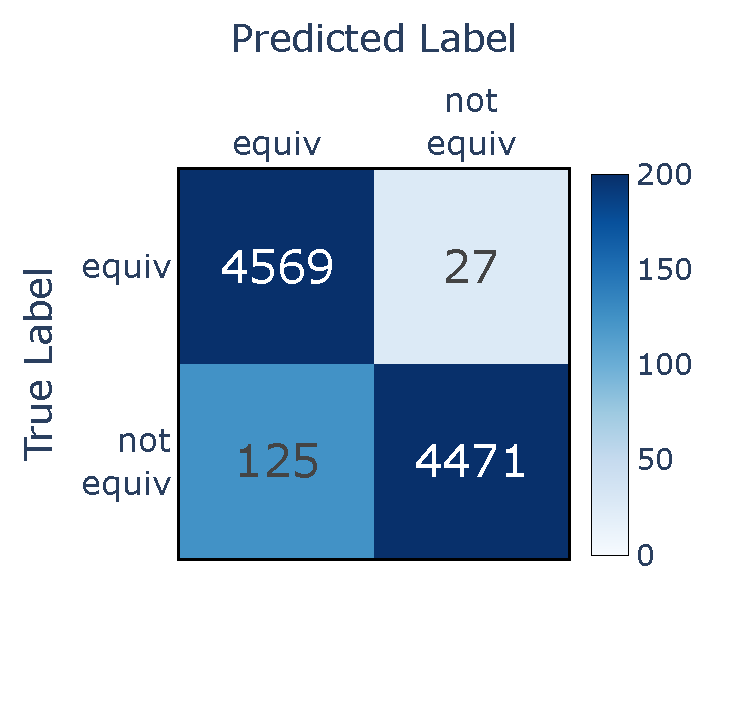
\includegraphics[width=0.246\textwidth,trim={29mm 23mm 7mm 0},clip]{cm_NVE_xgb.pdf}
    }
    \caption{NVE Confusion Matrices for Finalist Classifiers with Test Data}
\end{figure}

\begin{figure}[!h]
    \captionsetup{skip=5pt}
    \centering
    \captionsetup[subfigure]{oneside,margin={1.3cm,0cm}}
    \subfloat[KNN]{
        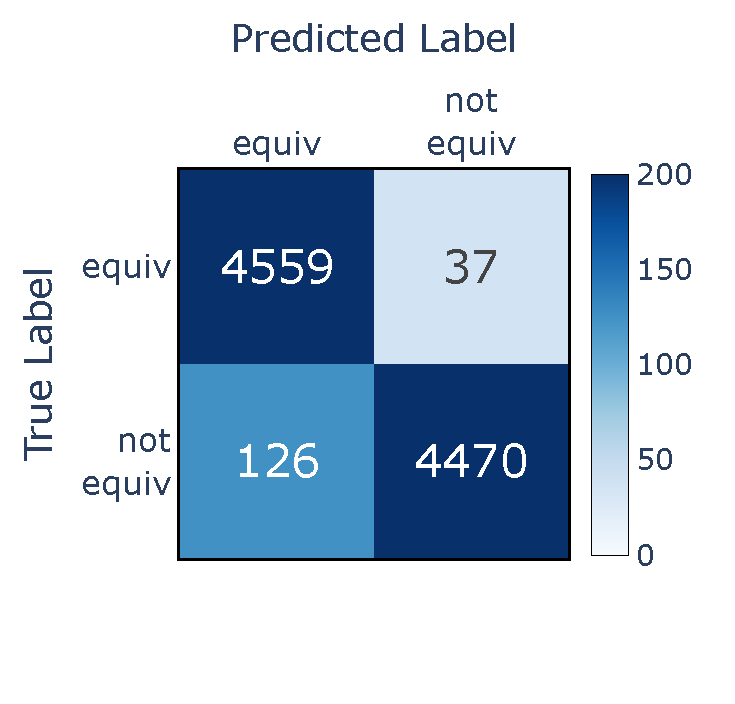
\includegraphics[width=0.277\textwidth,trim={0 23mm 26mm 0},clip]{cm_SFR_knn.pdf}
    }
    \captionsetup[subfigure]{oneside,margin={0cm,0cm}}
    \subfloat[Random Forest]{
        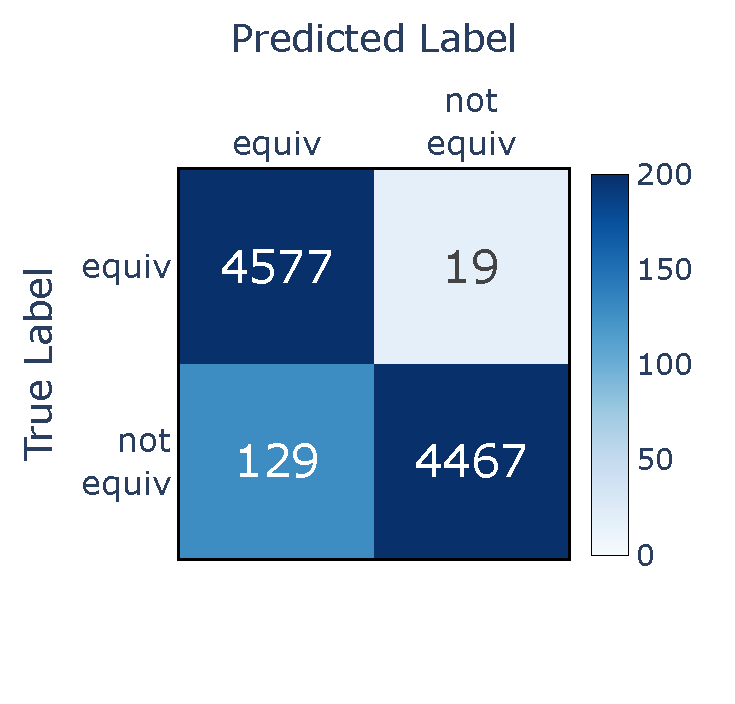
\includegraphics[width=0.194\textwidth,trim={29mm 23mm 26mm 0},clip]{cm_SFR_rf.pdf}
    }
    \captionsetup[subfigure]{oneside,margin={0cm,0cm}}
    \subfloat[SVM]{
        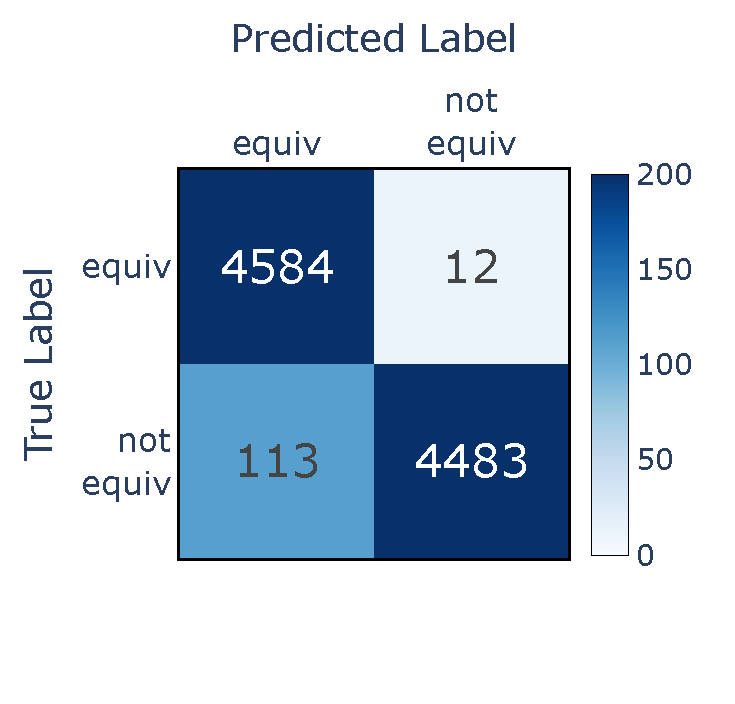
\includegraphics[width=0.194\textwidth,trim={29mm 23mm 26mm 0},clip]{cm_SFR_svm.pdf}
    }
    \captionsetup[subfigure]{oneside,margin={-1.25cm,0cm}}
    \subfloat[XGBoost]{
        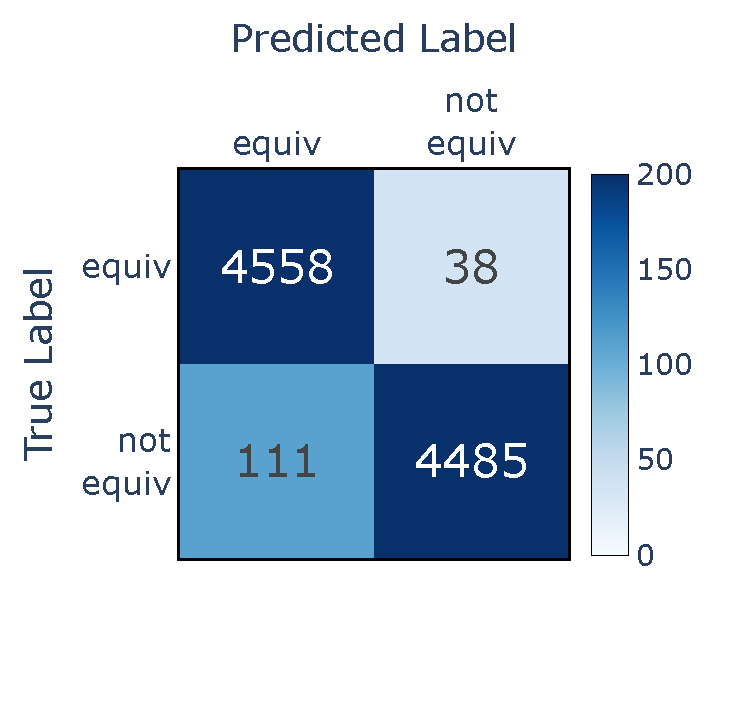
\includegraphics[width=0.246\textwidth,trim={29mm 23mm 7mm 0},clip]{cm_SFR_xgb.pdf}
    }
    \caption{SFR Confusion Matrices for Finalist Classifiers with Test Data}
\end{figure}


\chapter{Misclassification Analysis}
This appendix provides the full, unabridged text of representative misclassified course pairs discussed in Section~\ref{ch:4.6}, allowing for a direct, in-depth review of the error types.

\section{Most Misclassified Courses}\label{app:mostmiscls}
This is an inspection of the top 5 most misclassified courses across all classifiers and embedding models for both the training and test sets.

\begin{longtable}{ >{\baselineskip=12pt}c >{\baselineskip=12pt}p{0.9\textwidth} }
\captionsetup{skip=5pt}
\caption{Most Misclassified Courses (Training)}\label{tab:fp_overlap_training}\\
\toprule
\textbf{\textbf{Rank}} & \textbf{\textbf{Course}} \\
\midrule
\endfirsthead
\caption[]{Most Misclassified Courses (Training)}\\
\toprule
\textbf{\textbf{Rank}} & \textbf{\textbf{Course}} \\
\midrule
\endhead
1 & CID: ENGL-120 \newline
Santa Barbara City College \newline
ENG-222 Survey of British Literature \newline
Offered only in the Spring semester. Survey of British literature during 1798-present, including fiction, poetry, drama and essays. Prerequisite: ENG 110 or ENG 110H\\
\midrule
2 & CID: JOUR-130 \newline
Fullerton College \newline
JOUR-271 F Introduction to Spansh-Language Reporting \newline
Advisory: Understanding of conversational Spanish. 54 hours lecture and 18 hours lab per term. This course will guide students in the methods and styles of reporting and writing in Spanish for print and online. It will prepare students to publish stories and photos on the campus' Spanish-language publication. The course also provides students with a general understanding of contemporary Spanish-speaking and Latino communities. (CSU) (Degree Credit)\\
\midrule
3 & CID: PHYS-140 \newline
Berkeley City College \newline
CHEM-30A Introductory General Chemistry \newline
Fundamental principles of general chemistry: Metric measurements, matter and energy, atomic structure, chemical nomenclature, chemical bonding, chemical reactions, stoichiometry, gas laws, nuclear chemistry; properties of liquids, solids, solutions, acids, and bases.\\
\midrule
4 & CID: SOCI-125 \newline
Compton College \newline
SOCI-120 Introduction to Statistics and Data Analysis for the Behavioral Sciences \newline
This course introduces students to lesbian, gay, bisexual, transgender, and queer studies. It is designed to analyze power, privilege, and oppression in connection to current macro and micro dynamics in society. Students will evaluate significant historical LGBTQ+ events that fostered changing society's views on sexual identities, as well as, events that have worked against advancing LGBTQ+ rights. In addition, students will evaluate various theories and concepts that attempt to explain the social construction of gender, sex, and sexuality. Furthermore, students can analyze socialization, cultural values, norms, intersectionality, and the unique challenges that impact LGBTQ+ communities.\\
\midrule
5 & CID: PHYS-200 \newline
Foothill College \newline
PHYS-4A General Physics (Calculus) \newline
Mathematics-physics interrelationships, classical Newtonian mechanics. Lecture and lab hours indicated are per week. This course includes 5 lecture hours and 3 lab hours per week.\\
\bottomrule
\end{longtable}

\begin{longtable}{ >{\baselineskip=12pt}c >{\baselineskip=12pt}p{0.9\textwidth} }
\captionsetup{skip=5pt}
\caption{Most Misclassified Courses (Test)}\label{tab:fp_overlap_test}\\
\toprule
\textbf{\textbf{Rank}} & \textbf{\textbf{Course}} \\
\midrule
\endfirsthead
\caption[]{Most Misclassified Courses (Test)}\\
\toprule
\textbf{\textbf{Rank}} & \textbf{\textbf{Course}} \\
\midrule
\endhead
1 & CID: CDEV-100 \newline
Cerritos College \newline
CD-110 Child Development \newline
Examines the historical and current perspectives on diversity and inclusion and the impact of systemic societal influences on childrenÕs development, learning, and school experiences. Strategies for developmentally, culturally, and linguistically appropriate anti-bias curriculum will be explored as well as approaches to promote inclusive and anti-racist classroom communities. Includes self-reflection on the influence of teachersÕ own culture and life experiences on teaching and interactions with children and families.
Transfer Credit: CSU; UC\\
\midrule
2 & CID: ECE-230 \newline
Cerritos College \newline
CD-124 Teaching in a Diverse Society \newline
Introduces the appropriate use of assessment and observation tools and strategies to document young childrenÕ
s development and learning. The use of findings to inform and plan learning environments and experiences are
emphasized. Recording strategies, rating systems, portfolios, and multiple assessment tools will be
discussed, along with strategies for collaboration with families and professionals. 
Transfer Credit: CSU\\
\midrule
3 & CID: COMM-110 \newline
Saddleback College \newline
COMM-1 Communication Fundamentals \newline
Understand and use the processes of communication in making personal and social decisions in everyday life, including an understanding of problems and propositions; organization and development of ideas; evidence; methods of research, criticism and evaluation. Presentation of ideas in informative and persuasive contexts. Platform speaking experience will be required (formerly SP 1).\\
\midrule
4 & CID: CDEV-100 \newline
Cypress College \newline
PSY-145 C Child Psychology \newline
This course explores the physical, cognitive, communicative/linguistic, and socio-emotional development of the child from conception through adolescence across diverse cultures with an emphasis on the learning process. Education and teaching issues related to children are highlighted. (UC/CSU, AA GE, CSU GE, IGETC, CDEV 100)\\
\midrule
5 & CID: MUS-180 \newline
East Los Angeles College \newline
MUSIC-501 College Choir \newline
This course is an introduction to choral ensemble singing. Emphasis is on vocal technique and choral elements such as blend, intonation, diction, and music reading. Repertoire is chosen on the basis of group ability and represents historical and current styles of music. Students are required to perform in a public performance at the end of the semester.\\
\bottomrule
\end{longtable}

\section{False Positives: Topical Overlap}\label{app:topicoverlap}
This error occurs when courses cover the same broad subject but differ in critical dimensions such as academic level or their position in a curricular sequence. The model correctly identifies high semantic similarity but fails to capture the nuanced distinctions (e.g., Part I vs. Part II) that make the courses non-equivalent for articulation.

\begin{longtable}{ >{\baselineskip=12pt}p{0.45\textwidth} >{\baselineskip=12pt}p{0.45\textwidth} }
\captionsetup{skip=5pt}
\caption{FP Examples: Topical Overlap}\label{tab:fp_overlap_topic}\\
\bottomrule\toprule
\textbf{\textbf{Course A}} & \textbf{\textbf{Course B}} \\
\bottomrule\toprule
\endfirsthead
\caption[]{FP Examples: Topical Overlap}\\
\bottomrule\toprule
\textbf{\textbf{Course A}} & \textbf{\textbf{Course B}} \\
\bottomrule\toprule
\endhead
% Example 1: Sequential Physics
Evergreen Valley College \newline PHYS-004B (C-ID: PHYS-210) \newline General Physics & Foothill College \newline PHYS-4C (C-ID: PHYS-200) \newline General Physics (Calculus) \\
\midrule
This course is one of a three-semester series in calculus-based general physics, serving students majoring in engineering, chemistry, physics, mathematics and other sciences. It emphasizes conceptual aspects of electricity, magnetism, circuits, and Maxwell's equations, and requires quantitative analysis of real world situations. & Thermodynamics; mechanical, acoustical, and electromagnetic waves; optics. Lecture and lab hours indicated are per week. This course includes 5 lecture hours and 3 lab hours per week. \\
\bottomrule\toprule
% Example 2: Sequential English
East Los Angeles College \newline ENGLISH-205 (C-ID: ENGL-160) \newline English Literature I & East Los Angeles College \newline ENGLISH-206 (C-ID: ENGL-165) \newline English Literature II \\
\midrule
In this course, students read, discuss, and analyze major works of English literature from the Anglo-Saxon period to the late eighteenth century, to develop an understanding and appreciation of the poetry, fiction, and drama of these literary periods and to express that appreciation in a critical analysis. & This course surveys British Literature from the late 18th century emergence of the Romantics, such as Blake, Wordsworth, Coleridge, Byron, Shelley, and Keats; through the Victorian Era, writers such as Browning, Tennyson, Austen, Stevenson, Wilde, and Shaw; and into the early twentieth century, the rise of Modernism and after, writers such as Conrad, Eliot, Yeats, Woolf, Joyce, and Beckett. \\
\bottomrule\toprule
% Example 3: Intro vs. Bio-Psychology
Ventura College \newline PSY-V01 (C-ID: PSY-110) \newline Introduction to Psychology & Cabrillo College \newline PSYCH-4 (C-ID: PSY-150) \newline Introduction to Biological Psychology \\
\midrule
This course provides an overview of the scientific study of psychology in the areas of neuroscience, sensation and perception, states of consciousness, learning and memory, intellect and cognition, language, lifespan development and the influences of heredity and environment on behavior, motivation, sexuality, emotion, personality, stress and coping, psychological disorders, psychotherapy, and social relations. & Introduces the scientific study of the biological bases of behavior and its fundamental role in the neurosciences. Physiological, hormonal, and neurochemical mechanisms, and brain-behavior relationships underlying the psychological phenomena of sensation, perception, regulatory processes, emotion, learning, memory, and psychological disorders will be addressed. The course also notes historical scientific contributions and current research principles for studying brain-behavior relationships and mental processes. \\
\bottomrule\toprule
\end{longtable}

\section{False Positives: Ambiguous or Vague}\label{app:fpvague}
This error occurs when course descriptions are too brief or use generic, high-level language. This lack of specific detail increases ambiguity and can cause the model to identify semantic similarity between courses that are functionally distinct.

\begin{longtable}{ >{\baselineskip=12pt}p{0.45\textwidth}  >{\baselineskip=12pt}p{0.45\textwidth} }
\captionsetup{skip=5pt}
\caption{FP Examples: Ambiguous or Vague}\label{tab:fp_vague}\\
\bottomrule\toprule
\textbf{Course A} & \textbf{Course B} \\
\bottomrule\toprule
\endfirsthead
\caption[]{FP Examples: Ambiguous or Vague}\\
\bottomrule\toprule
\textbf{Course A} & \textbf{Course B} \\
\bottomrule\toprule
\endhead
% Example 1: Business Law
Cabrillo College \newline BUS-18 (C-ID: BUS-120) \newline Business Law & Long Beach City College \newline LAW-18 (C-ID: BUS-125) \newline Fundamental of Business Law \\
\midrule
Introduces the United States justice system, covering and relating criminal, civil, employment, torts and contract laws to business operations. History and nature of law, court systems, administrative agencies, crimes, cyber law, the formation and operation of contracts, corporate organization structures, ethical decisions and corporate responsibility and antitrust laws will be covered. & Formerly LAW 18A. This course is designed to explore the overall fundamental understanding of business law today. It examines the scope of how contracts and tort law affect the civil legal process as well as the nature of our current business environment. It is appropriate for students who wish to pursue a career in the business field. \\
\bottomrule\toprule
% Example 2: Communication
Cerritos College \newline COMM-132 (C-ID: COMM-140) \newline Fundamentals of Small Group Communication & Saddleback College \newline COMM-1 (C-ID: COMM-110) \newline Communication Fundamentals \\
\midrule
As an introduction to the fundamentals of group discussion, this course explores small group communication theories to examine group development; leadership in groups; group communication norms, and processes with emphasis on problem-solving, decision-making, and conflict-reduction techniques. Students will learn a variety of techniques to prepare and deliver group presentations. & Understand and use the processes of communication in making personal and social decisions in everyday life, including an understanding of problems and propositions; organization and development of ideas; evidence; methods of research, criticism and evaluation. Presentation of ideas in informative and persuasive contexts. Platform speaking experience will be required (formerly SP 1). \\
\bottomrule\toprule
\end{longtable}

\section{False Negatives: Semantic Divergence}\label{app:semdiv}
This error occurs when two officially equivalent courses (i.e., sharing a C-ID) are described using vastly different terminology or pedagogical focus. The model correctly assesses the texts as semantically dissimilar; the failure lies in the inconsistency of the source data, where the ground truth asserts an equivalence that is not clearly supported by the text.

\begin{longtable}{ >{\baselineskip=12pt}p{0.45\textwidth}  >{\baselineskip=12pt}p{0.45\textwidth} }
\captionsetup{skip=5pt}
\caption{FN Examples: Semantic Divergence}\label{tab:fn_divergence}\\
\bottomrule\toprule
\textbf{\textbf{Course A}} & \textbf{Course B} \\
\bottomrule\toprule
\endfirsthead
\caption[]{FN Examples: Semantic Divergence}\\
\bottomrule\toprule
\textbf{\textbf{Course A}} & \textbf{Course B} \\
\bottomrule\toprule
\endhead
% Example 1: CDEV-100
Bakersfield College \newline CHDV-B21 (C-ID: CDEV-100) \newline Child Growth and Development: Birth Through Adolescence & Cerritos College \newline CD-110 (C-ID: CDEV-100) \newline Child Development \\
\midrule
This introductory course examines the major physical, psychosocial, and cognitive/language developmental milestones for children, both typical and atypical, from conception through adolescence. There will be an emphasis on interactions between maturational processes and environmental factors. While studying developmental theory and investigative research methodologies, students will observe children, evaluate individual differences and analyze characteristics of development at various stages. & Examines the historical and current perspectives on diversity and inclusion and the impact of systemic societal influences on children’s development, learning, and school experiences. Strategies for developmentally, culturally, and linguistically appropriate anti-bias curriculum will be explored as well as approaches to promote inclusive and anti-racist classroom communities. Includes self-reflection on the influence of teachers’ own culture and life experiences on teaching and interactions with children and families. \\
\bottomrule\toprule
% Example 2: ECE-230
Cerritos College \newline CD-124 (C-ID: ECE-230) \newline Teaching in a Diverse Society & Oxnard College \newline ECE-R107 (C-ID: ECE-230) \newline Teaching in a Diverse Society \\
\midrule
Introduces the appropriate use of assessment and observation tools and strategies to document young children’s development and learning. The use of findings to inform and plan learning environments and experiences are emphasized. Recording strategies, rating systems, portfolios, and multiple assessment tools will be discussed, along with strategies for collaboration with families and professionals. & This course examines the impact of various societal influences on the development of children's social identity. Students encounter that diversity is a major cultural trait of the United States, and recognize that schools reflect the societal makeup of our country. The course includes an identification of the main differences and similarities among various cultural groups and those of the mainstream culture. \\
\bottomrule\toprule
% Example 3: SOCI-160
Santa Barbara City College \newline SOC-106 (C-ID: SOCI-160) \newline Sociology of Deviance & Fullerton College \newline SOC-292 F (C-ID: SOCI-160) \newline Introduction to Criminology \\
\midrule
Examination of deviance and social control in contemporary society, using the sociological perspective. Focuses on the social processes involved in the construction of deviance, and its functions and impacts on individuals and society. Covers interpersonal and family violence; mental disorders; deviant sexuality; drug and alcohol use; and property, white-collar and organized crime. & This course is a study of theories of crimes and criminal behavior, including an explanation of crime, its causes, and how crime is measured. Major sociological and social science theories will be explored surrounding the issues of crime and criminal behavior. \\
\bottomrule\toprule
\end{longtable}

\section{False Negatives: Incomplete or Vague}\label{app:fnvague}
This error arises when one or both course descriptions in an equivalent pair are too sparse or generic to provide sufficient textual signal for the model to establish a confident match. Unlike semantic divergence where both descriptions are detailed but different, here the issue is a lack of substantive, comparable information.

\begin{longtable}{ >{\baselineskip=12pt}p{0.45\textwidth}  >{\baselineskip=12pt}p{0.45\textwidth} }
\captionsetup{skip=5pt}
\caption{FN Examples: Incomplete or Vague}\label{tab:fn_incomplete}\\
\bottomrule\toprule
\textbf{Course A} & \textbf{Course B} \\
\bottomrule\toprule
\endfirsthead
\caption[]{FN Examples: Incomplete or Vague}\\
\bottomrule\toprule
\textbf{Course A} & \textbf{Course B} \\
\bottomrule\toprule
\endhead
% Example 1: Field Geography
Cypress College \newline GEOG-202 C (C-ID: GEOG-160) \newline Field Geography - Physical & Palomar College \newline GEOG-195 (C-ID: GEOG-160) \newline Regional Field Studies in Geography \\
\midrule
Each separate offering of this course will occur in a unique location, studying unique circumstances and conditions in the field. Each course will employ its own combination of technical equipment, scientific instruments, and geotechniques. All courses will study the basic conceptual materials, with modifications associated with the location and the specific conditions encountered at each season. & Extended field studies of the geography of selected regions. Emphasis upon field observation and interpretation of climate, meteorology, vegetation, soils, and landforms. \\
\bottomrule\toprule
% Example 2: Physics
Imperial Valley College \newline PHYS-200 (C-ID: PHYS-205) \newline General Physics I & Moorpark College \newline PHYS-M20A (C-ID: PHYS-205) \newline Mechanics Solids and Fluids \\
\midrule
This course is designed to give an understanding of the fundamental principles of physics in the area of mechanics. & Introduces the basic principles of the mechanics of solids and fluids. Uses calculus to develop the subject matter. Covers kinematics, Newtonian mechanics including rotational dynamics, work, energy, fluid statics and dynamics, and simple harmonic motion. \\
\bottomrule\toprule
\end{longtable}

\section{False Negatives: Data or Labeling Errors}\label{app:labelerror}
This error arises when othere is a data entry error or the label is incorrect.

\begin{longtable}{ >{\baselineskip=12pt}p{0.45\textwidth}  >{\baselineskip=12pt}p{0.45\textwidth} }
\captionsetup{skip=5pt}
\caption{FN Examples: Data Entry or Labeling Error}\label{tab:fn_entry}\\
\bottomrule\toprule
\textbf{Course A} & \textbf{Course B} \\
\bottomrule\toprule
\endfirsthead
\caption[]{FN Examples: Data Entry or Labeling Error}\\
\bottomrule\toprule
\textbf{Course A} & \textbf{Course B} \\
\bottomrule\toprule
\endhead
% Example 1: Field Geography
Santa Barbara City College \newline PSY-150 (C-ID: SOCI-125) \newline Statistics for the Behavioral Sciences & Compton College \newline SOCI-120 (C-ID: SOCI-125) \newline Introduction to Statistics and Data Analysis for the Behavioral Sciences \\
\midrule
Principles and procedures of measurement, data analysis, probability, sampling theory and statistical significance. Covers basic descriptive statistics, including measures of linear relationships and standard scores. Covers the logic of hypothesis testing and inferential statistics up to analysis of variance, including a conceptual introduction to factorial designs. Students conduct analyses by hand and computer software. & This course introduces students to lesbian, gay, bisexual, transgender, and queer studies. It is designed to analyze power, privilege, and oppression in connection to current macro and micro dynamics in society. Students will evaluate significant historical LGBTQ+ events that fostered changing society's views on sexual identities, as well as, events that have worked against advancing LGBTQ+ rights. In addition, students will evaluate various theories and concepts that attempt to explain the social construction of gender, sex, and sexuality. Furthermore, students can analyze socialization, cultural values, norms, intersectionality, and the unique challenges that impact LGBTQ+ communities.\\
\bottomrule\toprule
\end{longtable}

\end{document}
